\documentclass{book}

%%%%%%%%%%%%%%%%%%%%%%%%%%%%%%%%%%%%%%%%%%%%%%%%
% This seciont would include all the required
% packages.
%%%%%%%%%%%%%%%%%%%%%%%%%%%%%%%%%%%%%%%%%%%%%%%%
% package to wrap text around figures.
\usepackage{wrapfig}

% for pseudo-code
\usepackage{algorithmic}

% for argmin and argmax
% https://tex.stackexchange.com/a/5255
\usepackage{amsmath}
\DeclareMathOperator*{\argmax}{arg\,max}
\DeclareMathOperator*{\argmin}{arg\,min}

\usepackage{adjustbox}

% table of contents are in different lines.
\usepackage[utf8]{inputenc}

% for table's toprule and bottomrule
\usepackage{booktabs}

\usepackage{tikz}

% to include pdfpages
\usepackage{pdfpages}

% for table
\usepackage{multirow}

% code listing
\usepackage{tcolorbox}
\usepackage{listings}
\lstdefinestyle{mystyle}{
	backgroundcolor=\color{backcolour},   
	commentstyle=\color{codegreen},
	keywordstyle=\color{magenta},
	numberstyle=\tiny\color{codegray},
	stringstyle=\color{codepurple},
	basicstyle=\ttfamily\footnotesize,
	breakatwhitespace=false,         
	breaklines=true,                 
	captionpos=b,                    
	keepspaces=true,                 
	numbers=left,                    
	numbersep=5pt,                  
	showspaces=false,                
	showstringspaces=false,
	showtabs=false,                  
	tabsize=2
}
\lstset{style=mystyle}

% page dimensions
\usepackage{geometry}
\geometry{
	a4paper,
	total={170mm,257mm},
%	left=20mm,
%	top=20mm,
	left=1.5in,
	right=1in,
	top=1in,
	bottom=1in,
}

% captioned images or figures in LaTeX.
\usepackage{float}

% for referencing
\usepackage[%  
colorlinks=true,
pdfborder={0 0 0},
linkcolor=red
]{hyperref}

% to make caption bold.
% https://tex.stackexchange.com/a/32463/277097
\usepackage[labelfont=bf]{caption}

% increase spacing between paragraphs
\setlength{\parskip}{1mm}

% to number all the way down to subsections.
\setcounter{secnumdepth}{3}

% colorbox
% https://texdoc.org/serve/tcolorbox.pdf/0
\usepackage{tcolorbox}

% citations
\usepackage{cite}

% to left indent caption
% https://tex.stackexchange.com/a/275141
%\captionsetup{justification=justified,singlelinecheck=false}

%%%%%%%%%%%%%%%%%%%%%%%%%%%%%%%%%%%%%%%%%%%%%%%%
% package end.
%%%%%%%%%%%%%%%%%%%%%%%%%%%%%%%%%%%%%%%%%%%%%%%%

\title{
	Masterarbeit \\
	Robust Registration to a template brain  \\
	for the Drosophila larva \large }

\author{Harsha Yogeshappa}

% define RWTH Color
% https://www.color-hex.com/color-palette/33602
\definecolor{rwth-blue-1}{rgb}{0.00, 0.33, 0.62}
\definecolor{rwth-blue-2}{rgb}{0.25, 0.50, 0.71}
\definecolor{rwth-blue-3}{rgb}{0.55, 0.72, 0.89}
\definecolor{rwth-blue-4}{rgb}{0.78, 0.87, 0.95}
\definecolor{rwth-blue-5}{rgb}{0.90, 0.94, 0.98}
\definecolor{codegreen}{rgb}{0,0.6,0}
\definecolor{codegray}{rgb}{0.5,0.5,0.5}
\definecolor{codepurple}{rgb}{0.58,0,0.82}
\definecolor{backcolour}{rgb}{0.95,0.95,0.92}

% To change the color of chapter
% https://tex.stackexchange.com/a/75670
\usepackage{xcolor}
\usepackage{sectsty}
\chapterfont{\color{rwth-blue-1}}  % sets colour of chapters

% To change color of section headers.
\usepackage{titlesec}
\usepackage{color}

\titleformat{\section}
{\color{rwth-blue-1}\normalfont\Large\bfseries}
{\color{rwth-blue-1}\thesection}{1em}{}

\titleformat{\subsection}
{\color{rwth-blue-1}\normalfont\large\bfseries}
{\color{rwth-blue-1}\thesubsection}{1em}{}

\titleformat{\subsubsection}
{\color{rwth-blue-2}\normalfont\large\bfseries}
{\color{rwth-blue-2}\thesubsection}{1em}{}
% To change the color of caption
% \usepackage[font={color=rwth-blue-1},figurename=Figure]{caption}

% to include chapter name at the top of every page.
\usepackage{fancyhdr}

\fancyhf{} % clear all header and footer fields
\fancyhead[L]{\leftmark} % set the chapter name in the center of the header
\fancyfoot[C]{\thepage} % set the page number in the center of the footer
\pagestyle{fancy}

\usepackage{setspace}
\begin{document}
	\maketitle
	\cleardoublepage
	\newpage
	\vspace*{\fill}
	\begin{center}
		{\Large \textcolor{rwth-blue-1}{\textbf{Abstract}}}
	\end{center}
	In this work, we have addressed the problem of image registration of the larval brain of Drosophila that currently exists in the method known as \textit{larvalign}. The \textit{larvalign} method is a non-learning method for performing image registration that repeatedly encounters the same registration errors, particularly in the lower ventral nerve cord sections of the brain.
	
	To address these problems, we wanted to investigate whether a deep neural architecture such as Voxelmorph, known for its medical image registration capabilities, incorporated with landmark points as auxiliary information could help. We found that Voxelmorph alone could not handle large deformations in the scans. To overcome this limitation, we used a Gaussian pyramid-based approach and cascaded multiple Voxelmorph networks in a serial fashion and trained them with multi-resolution scans.
	
	Our results showed that cascading Voxelmorph networks in a multi-level and multi-resolution approach resulted in better registration accuracy than a single Voxelmorph network. Furthermore, our cascaded model trained with landmark information performed as well as the \textit{larvalign} method in terms of accuracy and was also able to handle scenarios where \textit{larvalign} failed. Our approach also significantly reduced the time required for registration, taking 35 seconds to register compared to 77 seconds for the \textit{larvalign} method on scans downscaled to 25\% of the original resolution. Our experiments have shown that our proposed method is also suitable for scans from other laboratories than the scans on which it was trained, making it more versatile and useful to a wider range of researchers.
	
	This research has significant implications for the field of image registration and the study of the larval brain of Drosophila, as it provides a general and robust approach that can be extended beyond the scans of a single laboratory in a much shorter time.
	\vspace*{\fill}
	
	\newpage
	
	\hypersetup{linkcolor=rwth-blue-1}
	\tableofcontents	

	\newpage
	
	\chapter{Introduction} \label{chap:intro}
	The purpose of this chapter is to introduce the main focus of this thesis and provide an overview of its key components. Specifically, we will present the background and motivation for this work, the specific objectives and hypotheses we are aiming to test, and the overall structure of the thesis. Our goal is to provide a clear and concise introduction to the content of the following chapters, giving the reader a clear roadmap for the rest of the document.
	
	% https://tex.stackexchange.com/a/8633/277097
	\section{Image Registration}
	Image registration is the process of aligning or registering two or more images so that they can be compared or combined. It is a fundamental technique in many fields, including medical imaging, computer vision, image processing, robotics, remote sensing, and computer graphics. Some examples of where image registration is used outside of medicine include:
	\begin{enumerate}
		\item \textbf{Computer vision}: Image registration is often used in computer vision to align images of the same scene or object, taken at different times or from different viewpoints, in order to facilitate image analysis and recognition tasks.
		\item \textbf{Image processing}: Image registration is used in image processing to correct for distortions or align images from different sensors or modalities. This is often done to improve the accuracy of measurements or to combine information from multiple sources.
		\item \textbf{Robotics}: Image registration is used in robotics to align images of the environment with a map or model of the environment in order to enable autonomous navigation.
		\item \textbf{Remote sensing}: Image registration is used in remote sensing to align satellite or aerial images of the earth's surface, taken at different times or from different platforms, in order to monitor changes or extract information about the environment.
		\item \textbf{Computer graphics}: Image registration is used in computer graphics to combine or align images or video frames in order to create seamless transitions or to generate special effects.
	\end{enumerate}
	
	Image registration is widely used in the field of medicine, particularly in medical imaging. Some examples of its applications in medicine include:
	
	\begin{enumerate}
		\item \textbf{Aligning medical images from different modalities}: Medical images are often taken using different imaging technologies, such as CT, MRI, PET, and ultrasound, which can produce images with different contrasts, resolutions, and field of views. Image registration is used to align these images in order to facilitate diagnosis and treatment planning.
		\item \textbf{Tracking the progression of a disease}: Image registration can be used to track the progression of a disease or the response to treatment by aligning medical images taken at different time points. This can be useful for monitoring the growth of a tumor, for example, or for evaluating the effectiveness of a treatment.
		\item \textbf{Fusion of medical images}: Image registration can be used to fuse medical images from different modalities in order to provide a more complete picture of the anatomy or physiology of a patient. For example, PET and CT images can be fused to combine functional and structural information.
		\item \textbf{Surgical planning and guidance}: Image registration can be used to align pre-operative images with real-time intra-operative images in order to guide surgical procedures or to assess the accuracy of a surgical approach.
		\item \textbf{Image-guided therapy}: Image registration can be used to align images of a patient's anatomy with images of a therapeutic device, such as a catheter or a radiation beam, in order to guide the delivery of treatment.
	\end{enumerate}
	
	There are many different techniques for image registration, including feature-based methods, intensity-based methods, and deformable registration methods.  Feature-based methods are recommended if the images contain distinctive and easily detectable features. This is usually the	case with remote sensing and computer vision where typically the image contains lot of details like roads, rivers, monuments etc. On the other hand, the medical images are not so rich in such details and thus intensity-based methods are usually employed. Sometimes, the lack of distinctive features in medical images are alleviated by introducing extrinsic features by an expert. Thus, the choice of technique depends on the specific needs of the application, such as the type and quality of the images being registered, the required accuracy of the registration, and the computational resources available.
	
	\subsection{Image Registration in the context of biological scans}
	Image registration is commonly used in the analysis of biological brain scans, such as those of Drosophila larva, to align images taken at different times, or using different imaging modalities, or to compare scans of different larvae. This allows researchers to compare and analyze the brain images in a common reference frame, which can provide valuable insights into the development and function of the brain.
	
	For example, image registration can be used to track changes in brain structure and function over time, such as during development or in response to different stimuli. It can also be used to combine information from different imaging modalities, such as fluorescence microscopy and electron microscopy, to create a more comprehensive view of the brain.
	
	In the context of Drosophila larva, image registration can be particularly useful for studying the development and function of the nervous system, as these insects have a relatively simple and well-defined nervous. Image registration can help researchers to align and compare brain images from different experiments or conditions, and to accurately measure and analyze changes in brain structure and function.
	
	% https://tex.stackexchange.com/a/8633/277097
	\begin{figure}[h!]
		\centering
		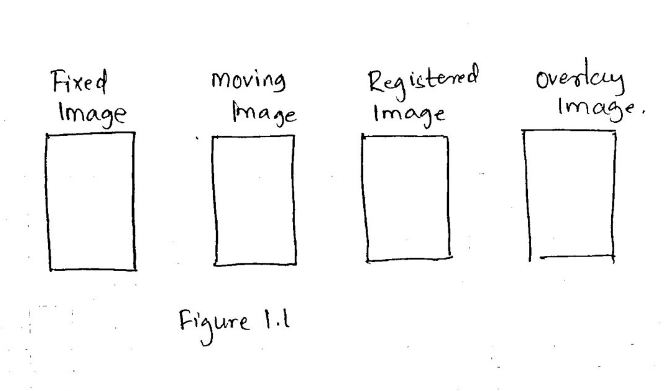
\includegraphics[width=\linewidth]{resources/chapter1/figure1.png}
		\caption{An image registration example}
		\label{fig:Registration}
	\end{figure}
	
	Figure~\ref{fig:Registration} shows an example of image registration of the Drosophila larva brain obtained using the \textit{larvalign} software \cite{larvalign}. In this example, image registration was used to align two brain scans of Drosophila larva, which were acquired as 3D volumes but are shown here as Maximum Intensity Projections (MIP) for illustrative purposes. The input scans are referred to as a fixed image and a moving image, and the output is a registered image with the moving image aligned to the fixed image. This alignment can facilitate the analysis of the images.
	
	\section{Motivation} \label{sec:motivation}
	Image registration can be broadly classified into two methods - deep learning methods and traditional methods. Both methods aim to align multiple images of the same or different objects, taken at different times or from different viewpoints. However, they differ in the approaches they take to achieve this goal.
	
	Traditional image registration methods typically rely on hand-crafted features or manually designed algorithms to align the images. On the other hand, image registration using deep learning methods relies on the use of neural networks to learn a mapping from the input images to the registered output. These methods can be more accurate and efficient than traditional methods, especially for complex images, as they are able to learn and adapt to the characteristics of the data. However, deep learning methods require a large amount of data for training. Traditional image registration can be prone to repeating errors and requires starting from scratch for each new image pair, whereas deep learning-based methods can learn from data and adapt to new image pairs more effectively.
	
	In this study, we aim to investigate the effectiveness of deep learning-based image registration in aligning brain scans of Drosophila larvae and compare it to the traditional method. We will also explore the possibility of using auxiliary information, such as landmark points, to guide the learning process and improve the accuracy and efficiency of image registration.
	
	The focus of this thesis is to build upon the work presented in the \textit{larvalign} paper \cite{larvalign}, which is a 3D volume template and a registration method for aligning brain scans of Drosophila larvae. While \textit{larvalign} showed promising results, it sometimes failed to accurately align images, particularly at the lower end of the ventral nerve cord (VNC) as shown in Figure \ref{fig:Registraion_Failure}.
	
	\begin{figure}[h!]
		\centering
		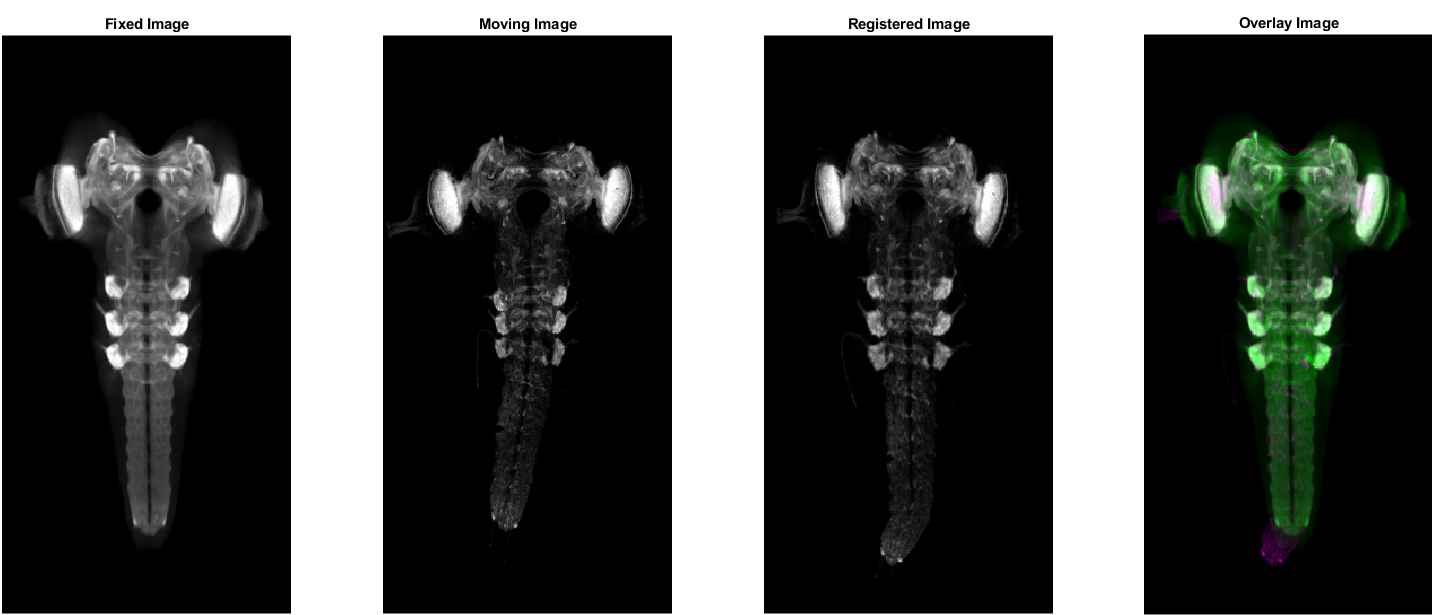
\includegraphics[width=\linewidth]{resources/motivation_fig_1.jpg}
		\caption{Brain scan of a larval specimen using the \textit{larvalign} registration method, showing failure in the lower end of the ventral nerve cord (VNC).}
		\label{fig:Registraion_Failure}
	\end{figure}
	
	Figure~\ref{fig:Registraion_Failure} contain the following information: 
	\begin{enumerate}
		\item The \textbf{Fixed or Template image} is the first image in the figure and is the image against which the registration is performed using the larvalign software.
		\item The \textbf{Moving or Subject image} is the second image in the figure and is the image that is being registered.
		\item The \textbf{Moved or Registered image} is the third image in the figure and is the result of the registration.
		\item The \textbf{Overlay image} is the fourth image in the figure and is an overlay between the fixed image and the moved image, which allows us to visually evaluate the quality of the registration.
	\end{enumerate}
	
	In the overlay image, green structures represent the fixed image and magenta structures represent the moved image. When the two images overlap perfectly, the intensity values are displayed.
	
	In this example case, the \textit{larvalign} software was unable to accurately align the moving image with the fixed image, as indicated by the protruding magenta structure at the lower end of the ventral nerve cord (VNC) in the overlay. This is an example of a case where \textit{larvalign} struggles to handle large deformations at the lower end of the ventral nerve cord (VNC) and consistently produces registration errors in these situations. This issue occurs repeatedly whenever we attempt to register these image pairs again.
	
	\textit{larvalign} is a non-learning method for image registration, which means it cannot improve with experience. We explore the use of a learning-based method of registration that can adapt and potentially outperform larvalign. Deep learning techniques have been effective at learning to compute the deformation field between image pairs \cite{Balakrishnan_2019, de_Vos_2019, Wu, Fu_2020, 10.1007/978-3-319-66182-7_27}, and we expect this approach to be more efficient in terms of registration time compared to \textit{larvalign}.
	
	In our image registration use case, registration is always performed using the same fixed reference image. This is an advantage because it allows consistency to be achieved across all training images. By using the same fixed image as a reference, the network can learn to align all images to a common coordinate system, which can improve the accuracy of the registration. With many training examples for the image registration problem, we can train the network in a supervised manner to learn from past registration and not repeat the same mistake.
	
	\section{Objectives and Hypothesis}
	The goal of this thesis is to investigate whether deep learning techniques like Voxelmorph \cite{Balakrishnan_2019} can be used to improve the robustness and efficiency of image registration for biological brain scans of Drosophila larvae that may exhibit large deformations. We hypothesize that deep neural network architectures have the ability to learn complex, inherent features and can therefore be as efficient as \textit{larvalign} \cite{larvalign} in terms of accuracy in registration. Furthermore, we believe that by training these networks with more data, we can avoid the errors made by \textit{larvalign} \cite{larvalign} and that the prediction time for image registration using deep learning will be significantly faster, due to the ability of these networks to learn a function for computing the deformation field between pairs of images.

	\section{Organization}
	Finally, in this section we provide an overview of the structure of the thesis, highlighting the main chapters and subtopics that we will cover. This will help the reader to understand the organization of the study and how each chapter contributes to the research question.
	
	\begin{itemize}
		\item \textbf{Literature review}: This chapter presents an overview of the existing research on the topic of the study, highlighting the main findings and debates in the field.
		\item \textbf{Drosophila larva biology and an overview of machine learning techniques}: This chapter provides an overview of Drosophila larva biology and a summary of the machine learning techniques that will be used in the study.
		\item \textbf{Implementations and Data Preparation}: This chapter describes the research design, sample, and data collection and analysis procedures used in the study. 
		\item \textbf{Methods}: This chapter provides the complete details of the methods used in this thesis to address the problem statement. It provides enough detail for readers to understand and replicate the study.
		\item \textbf{Results}: This chapter presents the findings of the study, including tables, figures, and other visualizations. In addition, we will conduct several ablation studies and report its results.
		\item \textbf{Discussion}: This chapter interprets and contextualizes the results of the study, discussing their implications and limitations in relation to the literature review and research question.
		\item \textbf{Conclusion}: This chapter summarizes the main findings and implications of the study, and will highlight the contribution of the research to the field. It also identifies areas for future research.
	\end{itemize}
	
	\chapter{Literature review}
	\label{chap:litreture}
	Over the past few decades, given the numerous applications of image registration, a plethora of methods have been proposed. Until the success of AlexNet \cite{AlexNet} in the 2012 ImageNet competition, many of the proposed methods formulated the registration problem as a physical problem to minimize the energy function \cite{THIRION1998243} \cite{536892} \cite{5193151} \cite{5338015} \cite{Avants2011ARE} \cite{1009381}. The success of AlexNet led to increased confidence in deep learning techniques and their widespread use in research.
	
	The adaptation to deep learning techniques led to exceptional performance results in many computer vision tasks such as object recognition, image segmentation, image classification, etc., which could not be achieved before, and the popularity of deep learning methods increased rapidly.
	
	Not surprisingly, the current state-of-the-art methods for image registration are also based on deep learning methods, which are also used in this work. Traditional optimization methods minimize the dissimilarity function (or maximize the similarity function) between the fixed image and the moving image with respect to the registration parameters in an iterative process. In modern deep learning methods, the model is trained to learn the mapping between the fixed image and the moving image by optimizing an objective or cost function to perform registration in a single shot rather than iteratively. Although the training process can be resource intensive, the time required to perform registration after training a model is much less than the time required to perform mathematical optimization from scratch for each new image pair. Therefore, the methods can generally be divided into two types: traditional non-learning methods and modern deep learning methods. We'll talk about these in the next two sections, \nameref{section:traditional} and \nameref{section:dl}.
	
	\section{Traditional methods}
	\label{section:traditional}
	
	Thirion's Demons algorithm \cite{THIRION1998243} has been a popular choice for deformable registrations since the beginning of this century due to its linear complexity and simple implementation. The main idea of this work was to consider the object boundaries in one image as a semipermeable membrane and allow the other image, considered as a deformable grid model, to diffuse through these semipermeable boundaries by the action of effectors called demons located at these boundaries. The concept of demons was introduced by Maxwell in the 19th century to illustrate a paradox in thermodynamics, and this concept has been successfully adapted to image processing. If we want to match a moving image \emph{M} with a fixed image \emph{F}, it is assumed that the contour of an object \emph{O} in \emph{F} is a membrane and several demons are scattered on the contours of this object \emph{O}. These demons act as local effectors, pushing the moving deformable model \emph{M} to the inside of \emph{O} if the corresponding point of \emph{M} is labeled ``inside" or to the outside of \emph{O} if it is labeled ``outside".
	Image matching is an iterative process to find the transformation form \emph{T} that is the  evolution of a family of transformations \{$T_0$, $T_1$, ..... $T_i$, ..\} $\subset$ $\tau$ (where $\tau$ is the set of admissible deformations).
	
	Starting from an identity deformation {$T_0$}, for each iteration, the elementary force for each demon at the object boundary of the fixed image is calculated. From all elementary forces of the demons, the deformation $T_{i+1}$ of $T_i$ is calculated. The following Figure~\ref{fig:demons} represents this iterative scheme.
	
	\begin{figure}[h!]
		\centering
		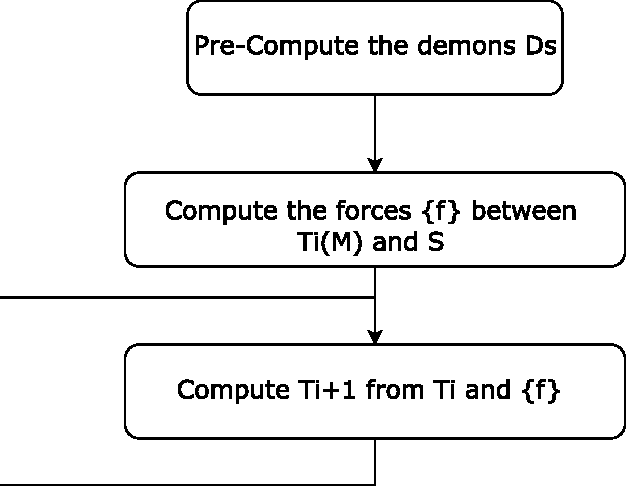
\includegraphics[width=0.7\columnwidth]{resources/chapter2/Demons.pdf}
		\caption{Iterative scheme in the case of diffusing models. \cite{THIRION1998243}}
		\label{fig:demons}
	\end{figure}
	
	One of the pioneering ideas in the field of large deformation registration was Christensen's modeling of the image as a fluid \cite{536892}. The image registration problem was formulated as a semilinear partial differential equation (PDE) system on the velocity field of the deformation, and it was shown how fixed point iteration generates a sequence of linear PDE systems. In \cite{5193151}, the demon algorithm was modified to perform curvature and fluid registration.
	
	There are a plethora of methods that have been proposed for image registration. Unfortunately, however, no universal method can be developed that is suitable for all registration problems. This may be due to the variety of images, assumed deformation types, required registration accuracy, application-dependent features, and other factors. To alleviate this problem, Klein et al. \cite{5338015} in 2010 developed a software toolbox called \emph{elastix} for intensity-based registration problems specifically used in medical image processing. The \emph{elastix} software contains various optimization methods, multiresolution methods, interpolators, samplers, transformation models, and cost functions which is very helpful for the user to quickly compare different registration methods and select a satisfactory configuration for a particular application. \emph{{larvalign}} \cite{larvalign} proposes such a method using \emph{elastix}. \emph{{larvalign}} \cite{larvalign} is an automatic and semi-automatic registration procedure, which is also the impetus for this thesis. In the following subsection, we shall talk more about what \emph{{larvalign}} is and the results it achieved.
	
	\subsection{\emph{larvalign}}
	\emph{{larvalign}} \cite{larvalign} is the stimulus for this work, i.e., this work is an extension of the work of \emph{{larvalign}} \cite{larvalign}. \emph{{larvalign}} \cite{larvalign} is both a standard template of the larval brain of the fruit fly \emph{Drosophila melanogaster} and an automatic and semi-automatic registration method for registering different scans of the larval brain to this standard template. The \emph{{larvalign}} \cite{larvalign} software package performs a specific sequence of image processing steps optimized specifically for the registration of microscopic images of the central nervous system (CNS) of third instar Drosophila larvae. The following is a brief overview of the registration algorithm, the evaluation of the results, and finally the results itself in \emph{{larvalign}} \cite{larvalign}.
	
	\subsubsection{Registration Algorithms}
	\label{subsubsection:registration_algo}
	Image registration in \emph{{larvalign}} is performed in two steps: global alignment of images (linear/affine/rigid registration) and local alignment of images (nonlinear/deformable/non-rigid registration).
	
	The global alignment serves as initialization for the nonlinear registration. During the acquisition of brain samples, the samples can be randomly aligned and also mirrored in the z-direction. The goal of global alignment is to ensure that these acquired brain scans (moving images) have approximately the same orientation, size, and are in the same slice order in the z-direction as the standard template larval brain.  Therefore, linear (affine) registration prior to nonlinear (deformable) registration would greatly facilitate the implementation of the non-rigid transformation.
	
	Local alignment was performed using both non-parametric methods (variational methods) and parametric methods (B-spline models). Both methods were empirically evaluated to select the best of the two. Both categories have their own state-of-the-art toolkit for biomedical image registration, \emph{ANTs} \cite{Avants2011ARE} and \emph{elastix} \cite{5338015}, where \emph{ANTs} image registration is best known for its symmetric diffeomorphic registration (SyN) algorithm \cite{Avants2008SymmetricDI}. An initial experiment was performed to \emph{ANTs} SyN and \emph{elastix} B-spline registration approach for pairwise nonlinear registration. Although comparable results were obtained with both methods, it was found that registration with \emph{ANTs} took more than 8 hours, whereas registration with \emph{elastix} took about 4 minutes. Since the goal was accurate and \emph{fast} image registration, the \emph{elastix} approach was chosen.
	
	\subsubsection{Assessment}
	\label{subsubsection:assessment}
	In addition to the visual inspection of the registered image, a quantitative value was defined to measure the quality of the registration. Although the correlation between the registered image and the fixed image captures the misalignment, such global measurements usually do not account for the local errors. To quantify local registration errors, statistical descriptors were developed for the regions at the entry points of the Ventral Nerve Cord (VNC) and thoracic nerve, similar to those used by Muenzing et al \cite{Muenzing},. These descriptors were defined as VNC Terminal Error Indicator (\textbf{VI}) and Thoracic Nerve Error Indicator (\textbf{TI}), respectively. If these indicators had a value of less than 50\%, this was an indication of a possible registration error. Apart from these two, another error called Landmark Registration Error (\textbf{LRE}) was defined, which was nothing but the average of the Euclidean distance between all landmarks in the fixed image and the registered image.
	
	Up to this point, registration is completely automatic and does not require human intervention. However, for those cases where \textbf{VI} and \textbf{TI} scored less than 50\%, a framework for registration based on landmarks was developed as a fallback strategy. In the event that VNC registration fails (\textbf{VI} score less than 50 \%), two landmarks were provided to guide this semi-automatic registration. In the event that thoracic registration failed (\textbf{TI} score less than 50 \%), six landmarks were placed at all six entry points of the thoracic nerve.	In contrast to automatic deformable registration, where only the correlation (NCC or MMI) between images controls the registration process, in semi-automatic deformable registration two similarity metrics control the registration process - the correlation metric and the Euclidean distance between the corresponding points \cite{inproceedings}.
	
	In the tabular data provided in \textit{larvalign} \cite{larvalign} it can be seen that for the partially failed registrations, landmark registration error (\textbf{LRE}) decreased after the semi-automatic registration was performed.
	
	\subsubsection{Results}
	\label{subsubsection:result}
	The proposed \emph{{larvalign}} registration method achieved an average landmark registration error (\textbf{LRE}) of \textbf{2.5 micrometers ± 1.5 micrometers} for the highest image quality data set, which is within the range of empirically measured human intra-rater variation measured on the same data set. However, the average landmark registration error (\textbf{LRE}) was \textbf{6.9 micrometers ± 6.4 micrometers} for the worst image quality within the representative data set, but it was noted that the intra-rater variation was measured on the high quality data and the baseline error could also be higher for the worst image quality data set.
	
	\section{Deep Learning Methods}
	\label{section:dl}
	
	Deep Learning (DL) belongs to a class of machine learning that uses neural networks with a large number of layers to learn the representation of the data and solve the task at hand. DL architectures had been limited in their ability to solve the then problems due to the vanishing gradient and the problem of overfitting. However, due to the availability of large datasets, large computational power in the form of GPUs and TPUs, and novel algorithms for training such deep networks, there has been a resurgence of interest in this concept. Recent works have also shown that they can even perform better than humans in some visual recognition tasks.
	
	When it comes to image registration, there are broadly three strategies that are prevalent in the current deep learning literatures: (1) using deep learning networks to estimate discriminate features for two images to drive an iterative optimization strategy, (2) using deep learning regression networks to directly predict transformation parameters, and (3) using deep learning networks to directly predict the deformation field. \cite{Litjens_2017}
	
	Wu et al. \cite{7314894} \cite{Wu} were the first ones to use deep learning to obtain application specific feature in contrast to the supervised feature extraction or handcrafted feature selection methods, and then the learnt features were deployed to the classical Demons \cite{VERCAUTEREN2009S61}, \cite{10.1007/10704282_64}, \cite{10.1007/978-3-540-85990-1_117}, \cite{10.1007/978-3-642-24446-9_3}, \cite{Peyrat} and HAMMER methods \cite{Wu2010TPSHAMMERIH}, \cite{Shen} with defined interpolation strategy, transformation model, and optimization alogirthm. These features were learnt from the data and hence is optimal representation for specific dataset. Thus, the then state-of-the-art registration methods were imporved by integrating these feature representations via deep learning. However, the registration process is still slow because the later transformation estimation is still iterative. Thus, methods to directly predict the transformation parameters have been proposed such that the registered image can be obtained directly by warping the moving image with the predicted transformation parameters.
	
	\begin{figure}[h!]
	\centering
	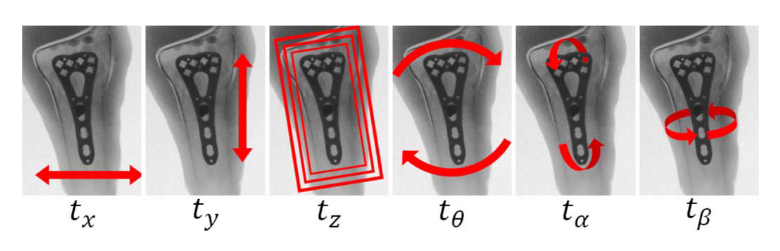
\includegraphics[width=0.7\textwidth]{resources/chapter2/tx_parameters.png}
	\caption{6 transformation parameters in a 3D transformation. \cite{7393571}}
	\label{fig:tx_parameters}
	\end{figure}
	
%	\begin{wrapfigure}{r}{0.5\textwidth}
%		\begin{center}
%			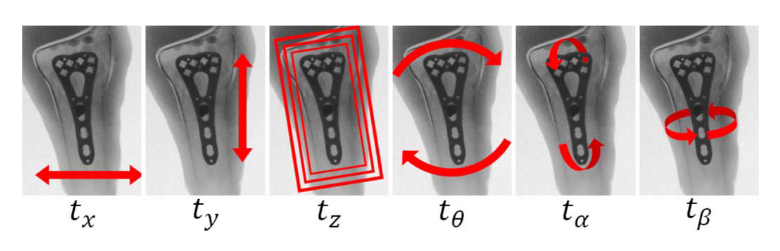
\includegraphics[width=0.5\textwidth]{resources/chapter2/tx_parameters.png}
%		\end{center}
%		\caption{6 transformation parameters in a 3D transformation. \cite{7393571}}
%		\label{fig:tx_parameters}
%	\end{wrapfigure}	
	
	Miao et al. \cite{7393571} were the first to use deep learning network to predict rigid transformation parameters. A rigid-body 3D transformation \emph{T} can be parameterized by a vector \emph{\textbf{t}} with 6 components of which 3 are in-plane (the translation parameters \emph{\textbf{$t_x$}} and \emph{\textbf{$t_y$}}, and rotation parameter \emph{\textbf{$t_\theta$}}) and 3 are out-of-plane (the translation parameter \emph{\textbf{$t_z$}} and rotation parameters \emph{\textbf{$t_\alpha$}} and \emph{\textbf{$t_\beta$}}) transformation parameters as shown in \ref{fig:tx_parameters}. A convolutional neural network (CNN) was used to predict the transformation parameters. Instead of regressing all parameters together, they were divided into three groups and regressed hierarchically.
	
	
	
	%\begin{wrapfigure}{r}{0.5\textwidth}
	%	\begin{center}
	%		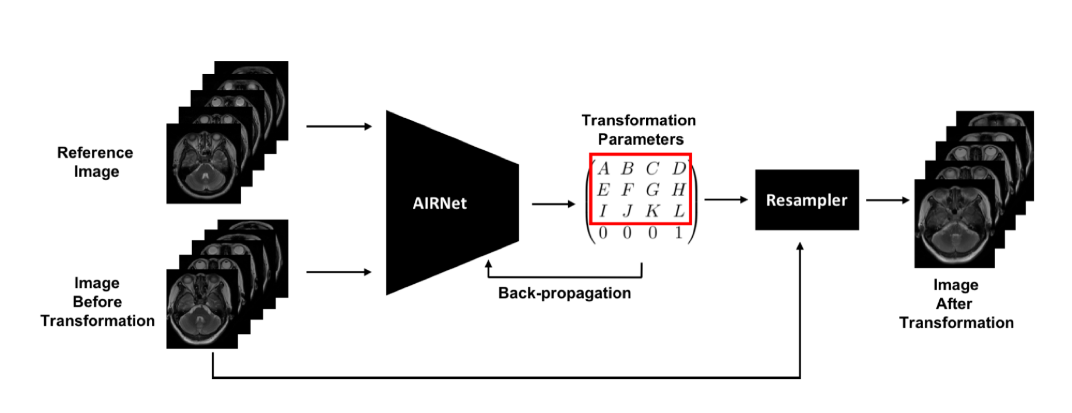
\includegraphics[width=0.5\textwidth]{resources/chapter2/AIRNet.png}
	%	\end{center}
	%	\caption{Workflow of \cite{https://doi.org/10.48550/arxiv.1810.02583} image registration framework.}
	%	\label{fig:AIRNet}
	%\end{wrapfigure}
	
	Chee et al. \cite{https://doi.org/10.48550/arxiv.1810.02583} employed a CNN to predict all transformation parameters simultaneously, rather than predicting them in groups and then applying them in a hierarchical fashion. In this framework, their Affine Image Registration Network (AIRNet) took two images and outputs the rigid transformation parameters. The moving image is then warped by the resampler using transformation matrix. The training loss function was mean-squared error of the estimated transformation parameters.
	
	%\begin{figure}[h!]
	%	\centering
	%	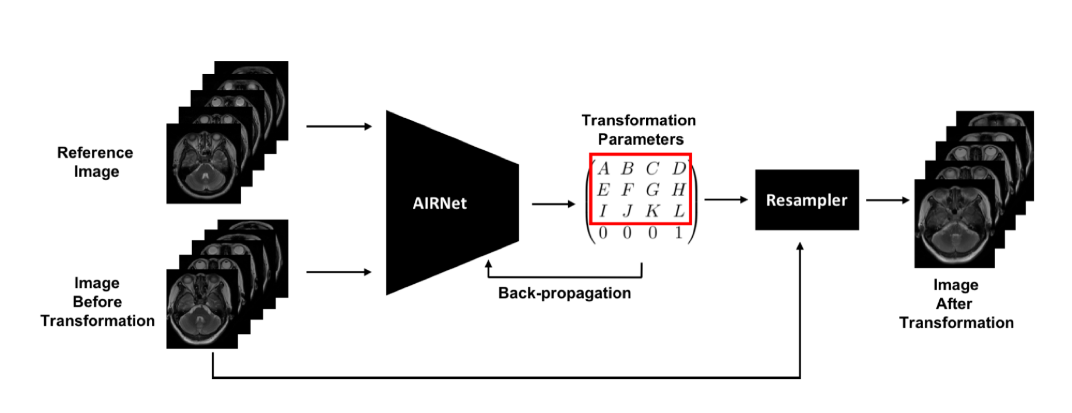
\includegraphics[width=0.7\columnwidth]{resources/chapter2/AIRNet.png}
	%	\caption{Workflow of \cite{https://doi.org/10.48550/arxiv.1810.02583} image registration framework.}
	%	\label{fig:AIRNet}
	%\end{figure}
	
	Yang et al. \cite{10.1007/978-3-319-46976-8_6}, Rohe et al. \cite{Roh2017SVFNetLD}, Jun et al. \cite{Jun}, Sokooti et al. \cite{10.1007/978-3-319-66182-7_27} and many others used deep learning approaches to predict the deformation field in a supervised fashion either with ground truth data or synthetic data.
	
	Interestingly, in one another work by Yang et al. \cite{https://doi.org/10.48550/arxiv.1804.11024}, Generative Adversarial Network was used to estimate the rigid transformation. Generator network was trained to predict the rigid transformation parameters, while the discriminator was trained to discern between the images that were warped with predicted transformation parameters and the images that were warped with the ground truth transformation parameters. Both Eucledian distance to ground truth and an adversarial loss term were used to construct the loss function.
	
	\subsection{Unsupervised Transformation Estimation}
	Despite the success of the above methods, the difficulty of obtaining reliable ground truth in the form of a warped image or deformation field is a major obstacle. This has motivated a number of research groups to explore unsupervised approaches. In this thesis also, an unsupervised approach is pursued, and thus this separate subsection is devoted to it in order to express its importance.
	
	A key innovation that has been useful for all work following the unsupervised method is the spatial transformer network (STN) \cite{NIPS2015_33ceb07b}. The spatial transformer network is a differentiable module that can be inserted into existing convolutional architectures, giving neural networks the ability to spatially transform feature maps. Since it is a differentiable module, it can also be trained together in an end-to-end fashion through backpropagation. In the paper, ``A Survey on Deep Learning in Medical Image Registration", \cite{Haskins_2020} a nice visualization aptly describes the workflow of unsupervised deep learning methods for registration.
	
	\begin{figure}[h!]
		\centering
		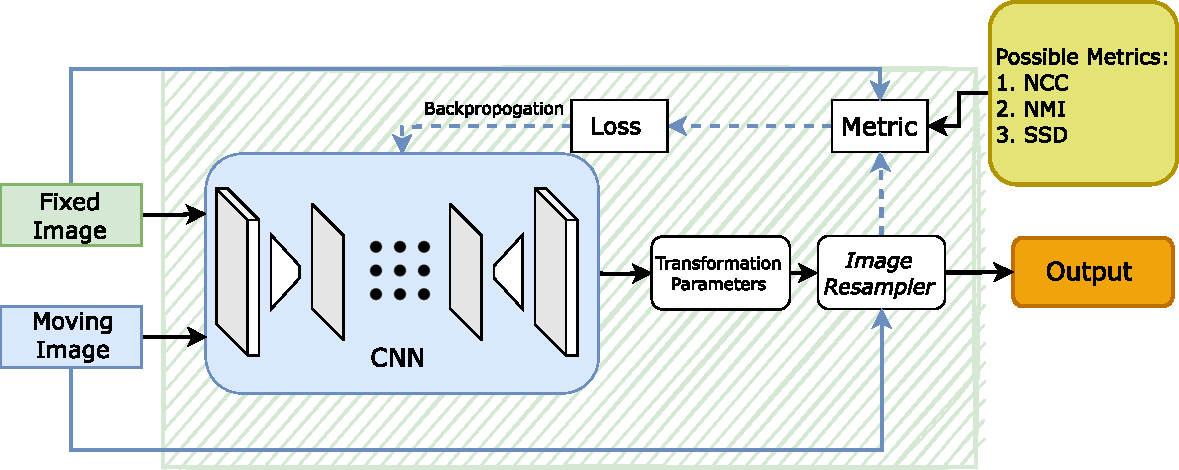
\includegraphics[width=0.9\columnwidth]{resources/chapter2/unsupervised_visualization.pdf}
		\caption{Visualization of unsupervised method of training deep neural networks for registration. \cite{Haskins_2020}}
		\label{fig:unsupervised_visualization}
	\end{figure}
	
	One of the important works in this area is by de Vos et al. \cite{de_Vos_2019}. In their work they proposed a Deep Learning Image Registration (DLIR) framework for unsupervised affine and deformable registrations. The framework is trained for image registration by exploiting image similarity between fixed and moving image pairs. In the DLIR framework, the transformation parameters are learnt by analysing the fixed and the moving image pairs. The predicted transformation parameters are then used to make a dense displacement vector field (DVF). DVF is used to resample the moving image into a warped image. Unlike many works that expects the moving image to be already to affinely aligned with the fixed image, the DLIR is designed for affine as well as deformable registration. Additionally, the framework also supports multi-stage ConvNets for registration of coarse-to-fine complexity in multiple-levels and multiple image resolutions by stacking ConvNets in a serial fashion. It is also said that such hierarchical mutli-stage strategy makes conventional iterative image registration less sensitive to local optima and image folding \cite{10.1007/3-540-45468-3_69}. Each stage is trained for its specific registration task, while keeping each of its weights fixed. After training, the multi-stage ConvNet is applied for one-shot image registration, similar to a single ConvNet.
	
	In the next section, the current state-of-the-art methods which are also unsupervised is explained in detail.
	
	\section{State-of-the-art methods}
	There are many proposed methods in the literature for learning a function for medical image registration using convolutional neural networks in an unsupervised manner. In this work, we consider some of these methods, which are the current state of the art, as base methods and adapt them to achieve a successful registration result for our larval brain scans.
	
	\subsection{VoxelMorph: An Unsupervised Learning Model for Deformable Medical Image Registration} 
	Like many other deep learning methods, the method proposed in VoxelMorph \cite{8579062} \cite{Balakrishnan_2019} also formulate registration as a function that maps an input image pair to a deformation field that matches the moving and fixed images. However, unlike other methods, two different training strategies were proposed in this work. In the first (unsupervised) setting, the model is trained to maximize the similarity between the fixed image and the registered image based on the image intensities. In the second setting, auxiliary information in the form of anatomical segmentations were used to steer the network in the right direction of learning. It was found that the model trained with auxiliary information performed better than the model trained without at the test time. The performance of both settings was comparable to the then state-of-the-art methods.
	
	3D MR scans of the human brain from healthy and sick people of different age groups were used for the study. In this work, more attention was paid to the slower deformable transformation than to the comparatively faster affine transformation. Therefore, it is assumed that the moving image and the fixed image are already affine aligned.
	
	The registration problem was formulated to find the optimal displacement vector field such that the dissimilarity between the fixed and registered images is the smallest. In addition, a smoothing loss was included to act as a regularizer to enforce a spatially smooth deformation.
	
	
	% https://oeis.org/wiki/List_of_LaTeX_mathematical_symbols
	% https://www.overleaf.com/learn/latex/Aligning_equations_with_amsmath
	\begin{equation} \label{loss_vxm}
	\begin{split}
	\hat{\phi} & = \argmin_\phi \mathcal{L}(f,m,\phi) \\
	& = \argmin_\phi (\mathcal{L}_{sim}(f,m \circ \phi) + \lambda \mathcal{L}_{smooth}(\phi))
	\end{split}
	\end{equation}
	
	where $m$ is moving image, $f$ is fixed image, $\phi$ is the deformation field, and $m \circ \phi$ represents $m$ warped by $\phi$, function $\mathcal{L}_{sim}(\cdot,\cdot)$ measures the similarity between the two input images, $\mathcal{L}_{smooth}(\cdot)$ imposes regularization, and $\lambda$ is the regularization trade-off parameter.
	
	The common metrics used for $\mathcal{L}_{sim}$ include intensity mean squared error, Normalized Cross-Correlation, and mutual information. The latter two are useful when volumes have varying intensity distributions and contrasts.
	
	\subsubsection{VoxelMorph CNN Architecture}
	
	The networks depicted in Figure~\ref{fig:vxm} and Figure~\ref{fig:vxm_unet} ar the same ones used in the VoxelMorph \cite{Balakrishnan_2019} study. It is included in this explanation for clarity. The network accepts both moving image $m$ and fixed image $f$ which is further concatenated into a 2 channel 3D image before fed to encoder-decoder architecture with skip connections. 3D convolutions in both the encoder and decoder stages use a kernel size of 3, a stride of 1, and same padding. Each convolution is followed by a leakyReLU layer with parameter 0.2. The convolution layers capture hierarchical features of the input image pair, to estimate $\phi$.
	
	In the encoder, max-pooling is performed to reduce the spatial dimensons in half at each layer. Thus, successive layers of the encoder operate over coarser representations of the input. This multilayer encoder network is used to transfer the high-dimensional 3D image patches into the low-dimensional feature representations.
	
	In decoder, alternate between upsampling, convolutions and skip connections are done. The decoder network is used to recover 3D image patches from the learned low-dimensional feature representations, acting as feedback to refine the inferences in the encoder network.
	
	\begin{figure}[h!]
		\centering
		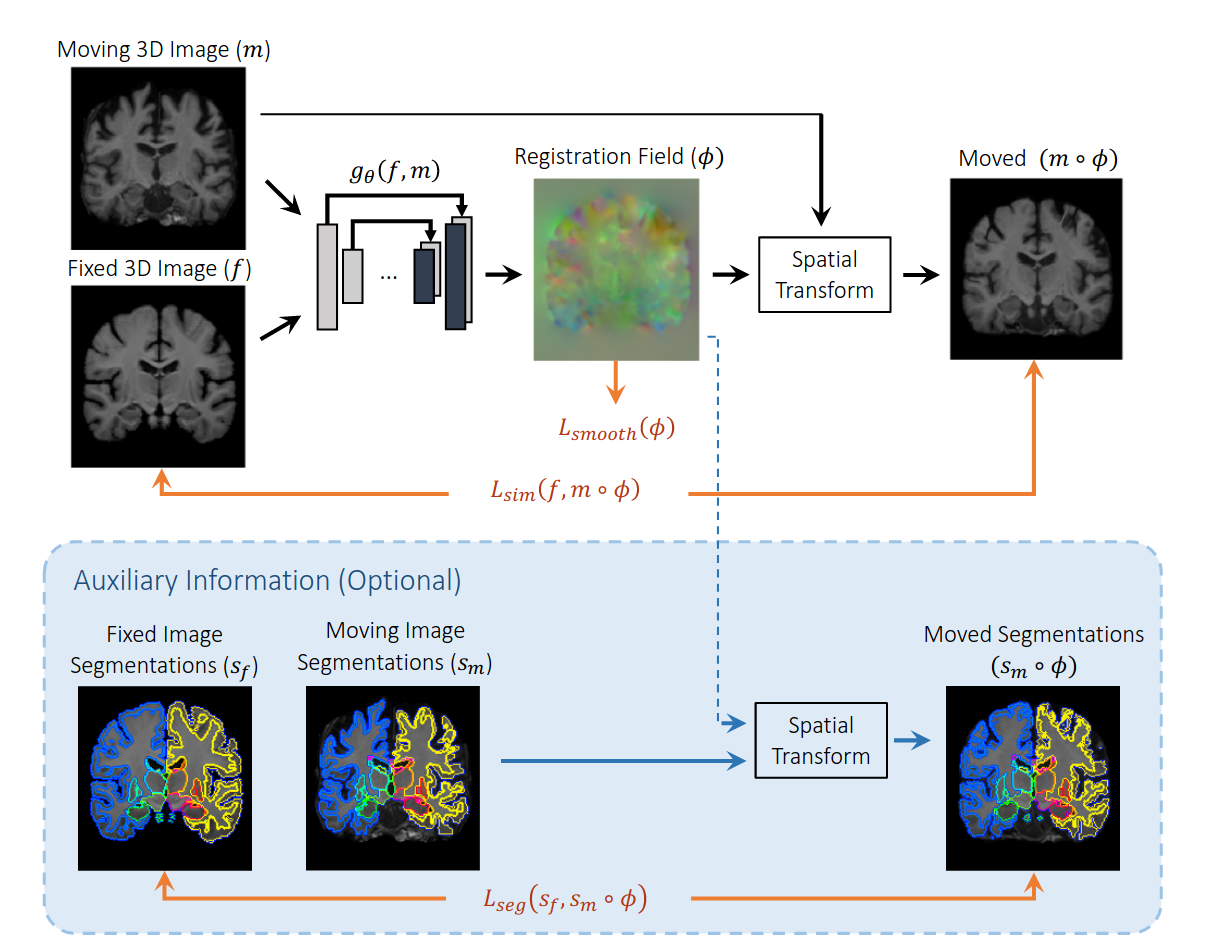
\includegraphics[width=0.9\columnwidth]{resources/chapter2/vxm.png}
		\caption{Overview of the VoxelMorph method. \cite{Balakrishnan_2019}}
		\label{fig:vxm}
	\end{figure}
	
	An important architectural constraint is that the receptive fields of the convolutional kernels of the smallest layer should be at least as large as the maximum expected displacement between corresponding voxels in $f$ and $m$.
	
	\begin{figure}[h!]
		\centering
		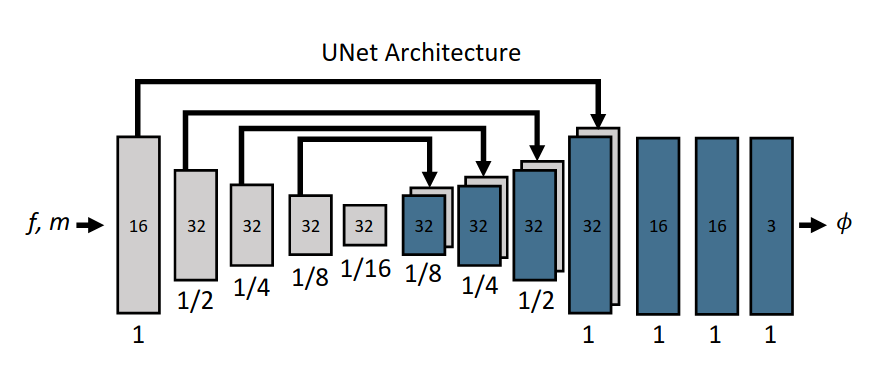
\includegraphics[width=0.8\columnwidth]{resources/chapter2/vxm_unet.png}
		\caption{Implementation of the U-Net convolution architecture. Each rectangle represents a 3D volume created from the previous volume using a 3D convolutional network layer. The spatial resolution of each volume with respect to the input volume is given below. Multiple 32-filter convolutions are used in the decoder, each followed by an upsampling layer to bring the volume back to full resolution. The arrows represent skip connections that chain encoder and decoder functions. \cite{Balakrishnan_2019}}
		\label{fig:vxm_unet}
	\end{figure}
	
	In another setup, the trained VoxelMorph was tested on the (unseen) Buckner40 dataset containing 39 scans. VoxelMorph with instance specific optimization was also performed. The dice scores in showed that VoxelMorph using cross correlation loss behaves comparably to ANTs and NiftyReg using the same cost function. Further, VoxelMorph with instance-specific optimization improved the results.
	
	Finally, the authors conclude that the VoxelMorph is a general learning model, and is not limited to any particular image type or anatomy - may be useful in medical image registration applications such as cardiac MR scans or lung CT images. Also, authors are of the opinion that with approporiate loss functions like mutual information, the model can also perform multimodal registration.
	
	\subsection{Cascade Networks for Unsupervised Medical Image Registration}
	Following the success of Voxelmorph \cite{Balakrishnan_2019}, improvised frameworks like Volume Tweening Network (VTN) \cite{8889674} and architectures like Recursive Cascaded Networks \cite{Zhao_2019} were proposed. Both the methods aimed at addressing the issues where the registration meant resolving large displacement fields.
	
	Although the authors note in the VoxelMorph paper \cite{Balakrishnan_2019} that the model may be useful for medical image registration applications such as MR scans of the heart or CT scans of the lung, Zhao et al. \cite{8889674} note that VoxelMorph does not work well when large shifts are present between images. Therefore, both papers \cite{8889674} and \cite{Balakrishnan_2019} offer a solution for dealing with such scenarios where large deformation fields are present by cascading the networks. In both the methods, final deformation field is a composition of field from the subnetworks. That is, the final flow prediction is composed of an initial affine transformation and $\phi_1$, $\phi_2$, $\cdots$, $\phi_n$, each of which only performs a rather simple displacement.
	
	Both VTN \cite{8889674} and DLIR \cite{de_Vos_2019} stack their networks. However, both are limited to a small number of cascades. DLIR trains each cascade one by one, i.e., after fixing the weights of previous cascades. VTN, in contrast, jointly trains the cascades measuring the similiarity between all successively warped images and the fixed image. Figure~\ref{fig:vtn} shows the Volume Tweening Network (VTN) \cite{8889674}. This network is the same one used in VTN paper \cite{8889674}, and is used in this explanation for clarity. Each registration subnet is responsible for determining the deformation field between the fixed image and the current moving image. The moving image is repeatedly distorted according to the deformation and fed into the next layer of cascaded subnetworks.
	
	\begin{figure}[h!]
		\centering
		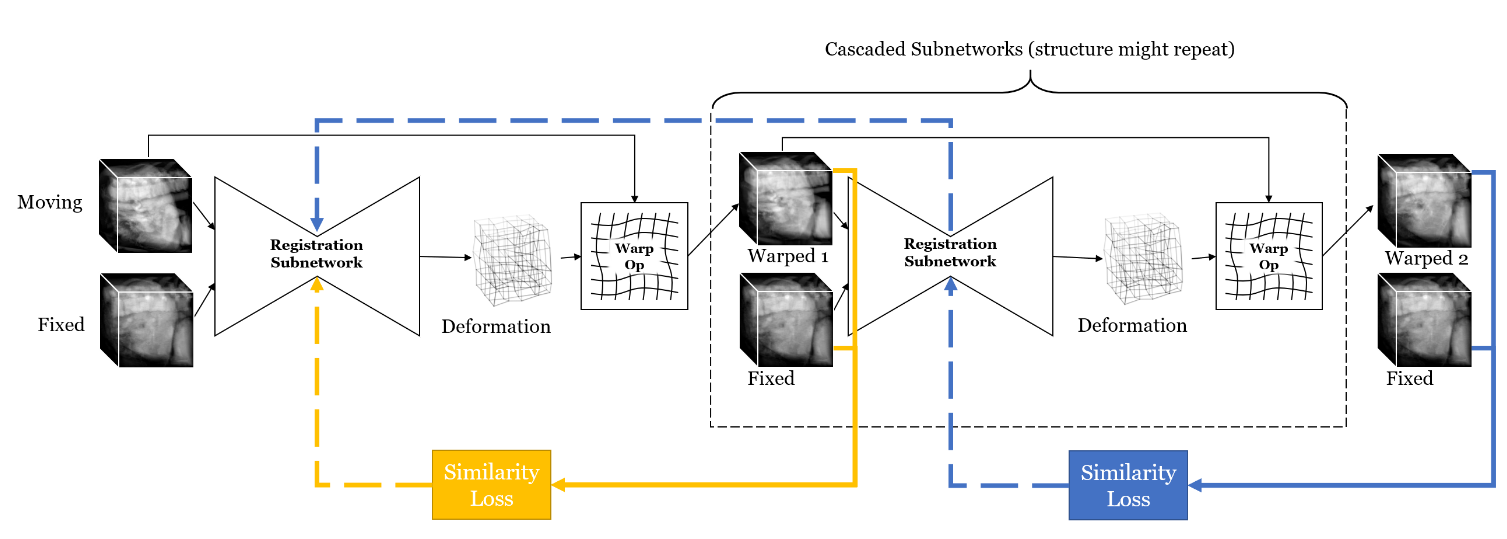
\includegraphics[width=\columnwidth]{resources/chapter2/vtn.png}
		\caption{Illustration of the overall structure of the Volume Tweening Network (VTN) and the back-progression of gradients. Solid lines indicate how the loss is computed and the dashed lines indicate how gradients back-propagate\cite{8889674}}
		\label{fig:vtn}
	\end{figure}
	
	Zhao et al. \cite{Zhao_2019} note that such a training method does not allow progressive registration of images. They refer to these as non-cooperative cascades because they learn their own targets independently of each other's existence, making further improvement unlikely even if more cascades are performed. Therefore, Zhao et al. \cite{Zhao_2019} propose the recursive cascade architecture, which allows unsupervised training of an unlimited number of cascades cascaded in a cooperative manner on any existing base network.
	
	The difference between this architecture and the VTN is that the similarity is now measured only on the final warped image, so that all cascades can learn progressive alignments together.
	
	It is shown that the performance of the recursive cascade network architectures for the SILVER, LiTS, and LSPG datasets against the base VoxelMorph and base VTN was better.
	
	
	After studying the literature, we decided to use VoxelMorph as the base model and incorporate concepts of VTN, DLIR, and recursive cascading networks for better performance. The cascading of the networks will be implemented in a coarse-to-fine fashion, similar to the image pyramid used in traditional image registration methods and proven for many years.

	\chapter{Drosophila larva biology and an overview of machine learning techniques}
	The Drosophila larva is a widely studied model organism in the field of biology, due to its short lifespan and ease of genetic manipulation. will provide an overview of the biological stages of Drosophila larva development and discuss their significance in the medical field. In addition, we will introduce the concepts of machine learning and deep learning, which are powerful techniques for analyzing and interpreting data. We will describe the key features and principles of these techniques, and how they are used in this thesis to address the research question.
	
	\section{Drosophila larva biology}
	Drosophila melanogaster, also known as the fruit fly, is a species of fly in the family Drosophilidae. Drosophila larvae, also known as maggots, are the immature stage of the fruit fly that precede the pupal stage and adult stage. They are commonly used as a model organism in genetics and developmental biology research due to their relatively simple nervous system, short generation time, and the availability of genetic tools for manipulating them.
	
	Drosophila larvae are small, legless, and worm-like in appearance, with a length of about 5 mm. They are typically white or yellow in color and have a segmented body with three main regions: the head, thorax, and abdomen. The head of the larva contains the brain, eyes, and mouthparts, while the thorax and abdomen contain the respiratory, circulatory, and digestive systems.
	
	During the larval stage, Drosophila undergoes significant changes in both form and function. For example, the larva grows in size, develops specialized organs and tissues, and undergoes metamorphosis to transform into the pupal stage. The larval stage is also a critical period for the development of the nervous system, with the formation and differentiation of neurons and glial cells, as well as the establishment of neural connections.
	
	\begin{figure}[h!]
		\centering
		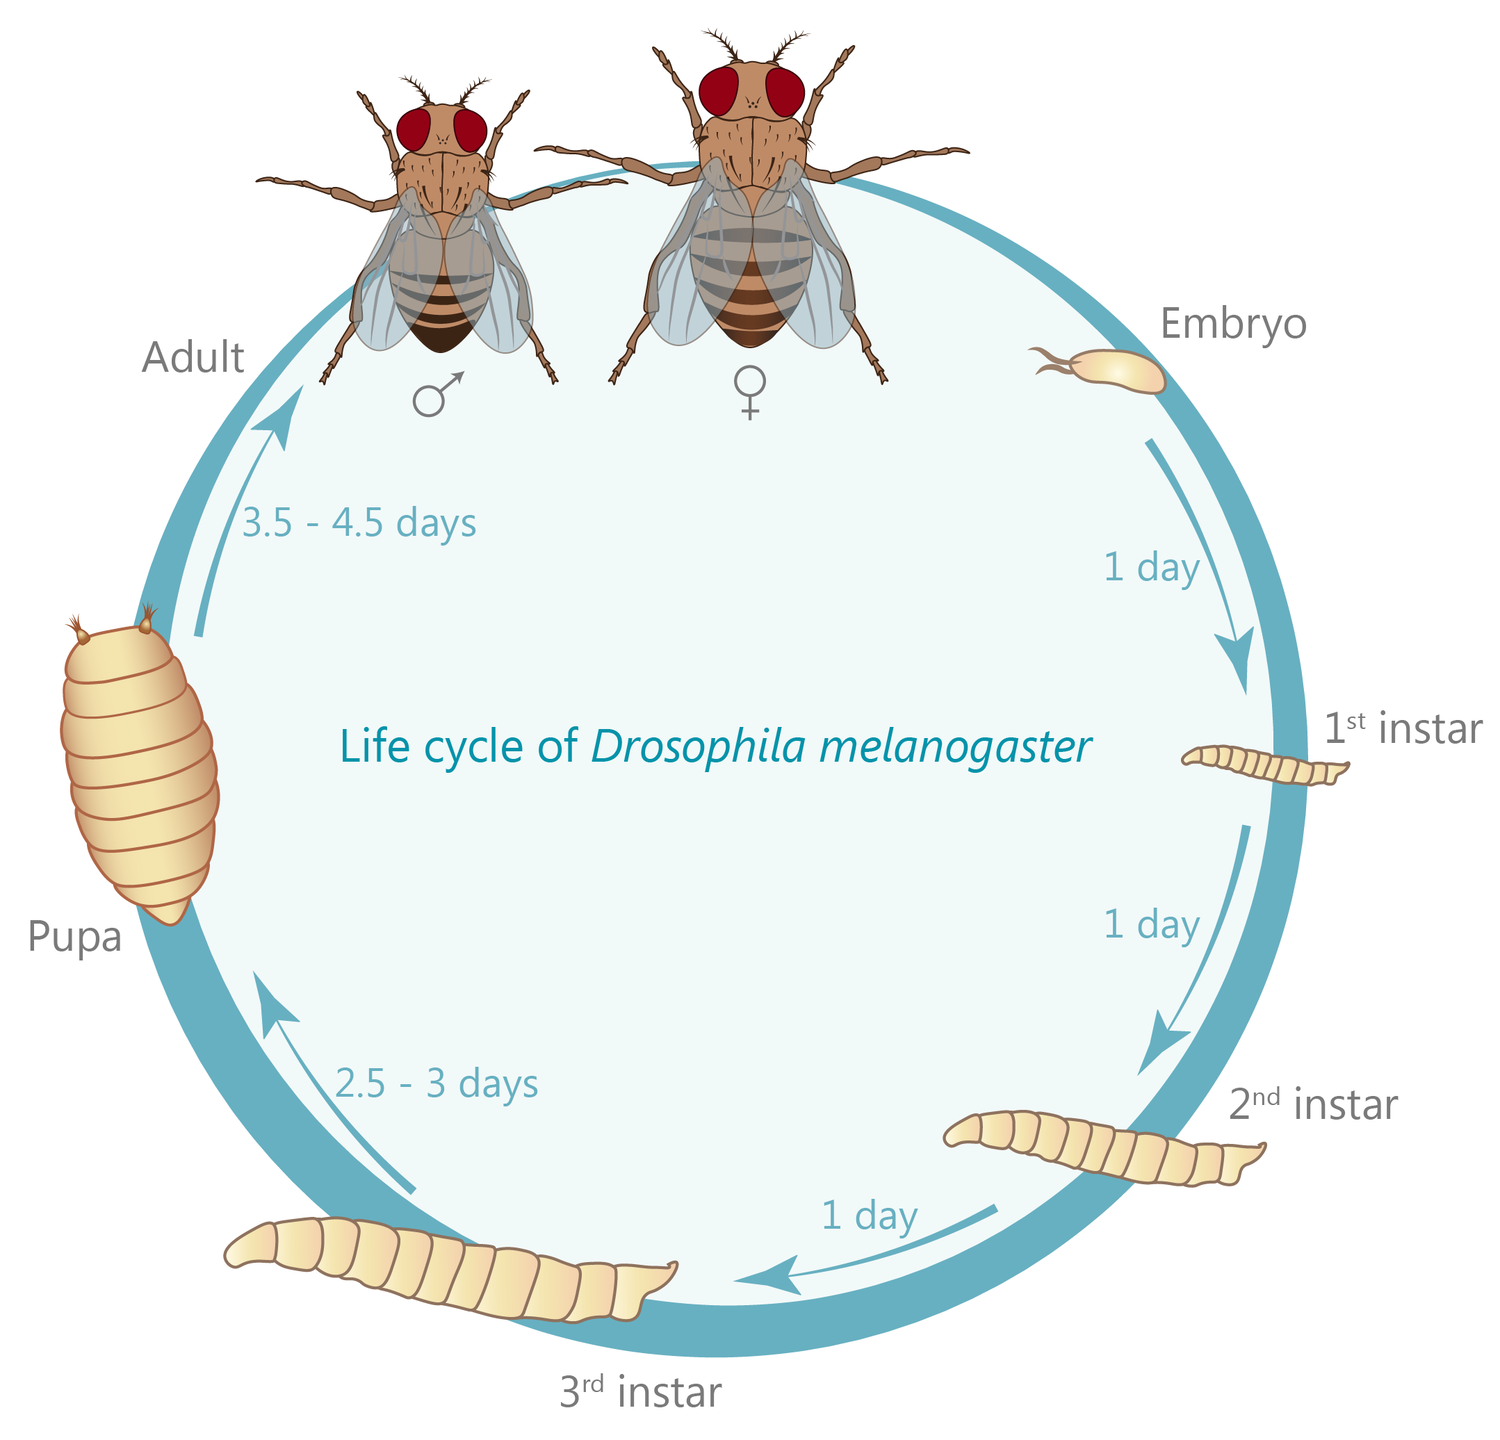
\includegraphics[width=0.7\columnwidth]{resources/model_organism_fig_1.png}
		\caption{Life \textbf{cycle} of Drosophila melanogaster. \cite{example_website}}
		\label{fig:Life_cycle_of_fruit_fly}
	\end{figure}
	
	Drosophila melanogaster undergoes a complete metamorphosis during its life cycle, which consists of four stages: egg, larva, pupa, and adult.
	
	\begin{enumerate}
		\item \textbf{Embryo}: The embryo stage is the first stage of Drosophila development. Drosophila eggs are small and oval-shaped, with a length of about 0.5 mm. They are laid singly or in clusters on moist surfaces, such as rotting fruit or moist soil. The egg contains a single cell that divides rapidly to form a multicellular embryo.
		\item \textbf{Larva}: The larva is the second stage of Drosophila development. Drosophila larvae, also known as maggots, are small, legless, and worm-like in appearance, with a length of about 5 mm. They are white or yellow in color and have a segmented body with three main regions: the head, thorax, and abdomen. The larva feeds on a variety of food sources, including rotting fruit, yeast, and other organic matter. During the larval stage, Drosophila undergoes significant changes in both form and function, including the growth of specialized organs and tissues and the development of the nervous system.
		\item \textbf{Pupa}: The pupa is the third stage of Drosophila development. Drosophila pupae are typically about the same size as the larva, but are more solid and have a more defined shape. They are typically dark in color and are enclosed in a hard, protective casing known as the puparium. During the pupal stage, Drosophila undergoes a process of metamorphosis, in which the larva transforms into the adult form. This process involves the reorganization and differentiation of tissues and organs, as well as the development of wings and other adult structures.
		\item \textbf{Adult}: The adult is the fourth and final stage of Drosophila development. Drosophila adults are small flies with a length of about 4-7 mm. They have a distinctive appearance, with a yellow or tan thorax, a black abdomen, and red eyes. Drosophila adults are sexually mature and are capable of reproducing. They feed on a variety of food sources, including fruit, nectar, and other sweet substances.
	\end{enumerate}
	
	\section{Drosophila larva as model organism}
	Drosophila larva are an important model organism in biology research due to their relatively simple nervous system, short generation time, and the availability of genetic tools for manipulating them. These characteristics make Drosophila larvae a useful tool for studying development, genetics, and neurobiology.
	
	
	\begin{enumerate}
		\item Drosophila larvae has relatively simple nervous system, which consists of about 100,000 neurons, compared to the approximately 100 billion neurons in the human brain. This simplicity makes it easier to study the development and function of the nervous system, as well as the underlying genetic and molecular mechanisms that regulate these processes.
		\item Drosophila larvae also have a short generation time, with a lifespan of about two weeks from egg to adult. This allows researchers to study development and evolution in a relatively short time frame, making Drosophila an important tool for studying the genetic basis of development and evolution.
		\item In addition, Drosophila larvae are amenable to genetic manipulation, allowing researchers to study the function of specific genes and pathways in development and behavior. For example, researchers can use techniques such as knockdown, overexpression, and gene editing to study the role of specific genes in the development and function of the nervous system.
	\end{enumerate}	
	
	These characteristics make Drosophila larvae a valuable tool for studying development, genetics, and neurobiology, and for identifying potential therapeutic targets for treating human diseases. While the brain of Drosophila larvae is certainly different from the human brain in terms of size, complexity, and overall organization, it shares many fundamental features and molecular pathways with the human brain.
	\begin{itemize}
		\item Like the human brain, the Drosophila larval brain contains various types of neurons and glial cells that perform different functions, and it is organized into distinct regions that are involved in specific behaviors and functions.
		\item Furthermore, the development and function of the Drosophila larval brain are regulated by many of the same genes and molecular pathways that regulate the development and function of the human brain. For example, many of the signaling pathways and transcription factors that regulate the development and function of the human brain are also present in the Drosophila larval brain.
	\end{itemize}
	
	Overall, studying the brain of Drosophila larvae can provide valuable insights into the fundamental processes that underlie the development and function of the nervous system, and may help to identify potential therapeutic targets for treating neurological disorders in humans.
	
	\section{Machine Learning and Deep Learning Background}
	This section discusses the concept of machine learning, as well as its subfield, deep learning, and the techniques and tools used to train models in this field. Deep learning is a type of artificial intelligence and machine learning that allows a computer to learn from experiences and perform well on new tasks, just like a human brain. This approach can be used to discover patterns and correlations through observations without human intervention and has been applied in various fields, including computer vision, speech recognition, natural language processing, and medical image processing. The following subsections provide more information on key deep learning techniques that are important to understand in the context of this thesis.
	
	\subsection{Machine Learning and types}
	Machine learning is a branch of AI that deals with improving the computer algorithms from experience and data without being explicitly programmed \cite{koza1996automated}. There	are four types of machine learning - supervised learning, unsupervised learning,semi-supervised learning, and reinforcement learning.
	In supervised learning, the algorithm or the model is trained using labeled data.
	During the training procedure, the model learns the parameters and uses these parameters to predict the outputs for unseen data. Supervised learning is of two types - regression and classification. Regression deals with continuous outputs whereas classification deals with discrete outputs. Supervised learning can be used in many applications like spam detection, object recognition, bioinformatics, etc. Though it has the above advantages, it may not generalize well to new data (overfitting), and pre-processing is a big challenge \cite{suplngdetails}.
	In unsupervised learning, the model is trained on unlabeled data to identify the
	hidden patterns and structures within the data. Unsupervised learning is also referred to as clustering. Some popular unsupervised learning algorithms are autoencoders, principal component analysis, etc. It is widely used for dimensionality reduction and exploratory analysis. The problems with unsupervised learning are that the results have high uncertainty and it is challenging to verify the outputs \cite{unsuplngdetails}.
	Semi-supervised learning is a combination of both supervised and unsupervised
	learning paradigms. The model is trained initially with the labeled data in a supervised fashion. Then unlabeled data is given to the model to predict the outputs.
	
	Later the predicted outputs are considered as the true outputs for the unlabeled data. Then the model has trained again with the combined data along with the labels. This method is helpful when we have limited labeled data. They are widely used in image and document classification tasks \cite{yoon2017semi}. Reinforcement learning works based on rewards and penalties. The goal of the model is to maximize the total reward. The model will not be given any labels, it has to figure out using trial and error approaches to come up with a solution to the problem. It gets feedback from the environment. Q-learning and Markov decision process are some of the most widely used reinforcement algorithms \cite{sutton2018reinforcement}.
	Even though machine learning algorithms have a lot of applications, they fail to perform well in image processing, natural language processing (NLP), etc. This is where deep learning is so powerful.
	
	\subsection{Deep Learning}
	Deep learning is a subset of machine learning that is inspired by the structure and function of the brain, specifically the neural networks that make up the brain. Deep learning algorithms are designed to learn and extract features from data automatically, rather than being explicitly programmed with a set of rules or features to look for.
	
	Deep learning algorithms are implemented using artificial neural networks, which are composed of multiple layers of interconnected artificial neurons, or ``perceptrons." These neural networks are trained using large amounts of labeled data and a variant of the backpropagation algorithm, which adjusts the weights of the connections between the neurons based on the error between the predicted output and the actual output.
	
	Deep learning algorithms are capable of learning complex, non-linear relationships in data and have been shown to achieve state-of-the-art results in a wide variety of tasks, including image and speech recognition, natural language processing, and predictive modeling. They have been applied to a wide range of applications, including self-driving cars, medical diagnosis, and language translation.
	
	One of the key benefits of deep learning is that it can learn to extract meaningful features from raw data, without the need for manual feature engineering. This can save a lot of time and effort in the preprocessing stage of a machine learning project, and can often lead to better performance on the task at hand. However, deep learning algorithms can be computationally expensive to train and require a large amount of labeled data to be effective.
	
	\subsection{Neural Networks}
	Neural networks or artificial neural networks (ANN) are the core of deep learning
	algorithms, whose name and design are inspired by how neurons function in the
	human brain. It can learn and model non-linear and complex relationships between
	input and output. It also has the ability to generalize, which implies it can infer
	associations from unobserved data after training.
	
	Neurons or perceptrons \cite{rosenblatt1958perceptron} are the basic blocks of a neural network. A perceptron takes a set of weighted inputs, exerts an activation function, and returns an output value. \ref{fig:Single Perceptron} illustrates the model of a perceptron. It takes any number of inputs (xi), which are weighted with corresponding weights (wi) and then summed up along with a bias (b). Then the sum is subjected to an activation function ($\sigma$) to produce the final output as shown in Equation \ref{eq:perceptron}. 
	
	\begin{equation}
	y = \sigma\left(\sum\limits_{i=1}^{n} w_i x_i + b\right) \label{eq:perceptron}
	\end{equation}
	
	In this equation \ref{eq:perceptron}., y is the output of the perceptron, x\_1, x\_2, ..., x\_n are the input features, w\_1, w\_2, ..., w\_n are the weights, and b is the bias term. The sigmoid function $\sigma$(x) is defined as:
	
	\begin{equation}
	\sigma(x) = \frac{1}{1 + e^{-x}}
	\end{equation}
	
	\begin{figure}[h!]
		\centering
		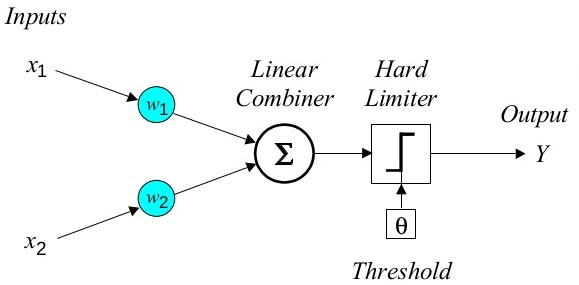
\includegraphics[scale=0.5]{resources/chapter3/perceptron.jpg}
		\caption{Illustration of model with a single perceptron. \cite{kamdem2023inputs}}
		\label{fig:Single Perceptron}
	\end{figure}
	
	Several perceptrons can be combined to solve more complex problems. Such a
	combination of neurons, which are organized in layers called multi-layer perceptrons (MLPs) as shown in \ref{fig:Multilayer Perceptron}. A multi-layered perceptron (MLP) is a type of artificial neural network that is composed of multiple layers of artificial neurons, or ``perceptrons." MLPs are used for supervised learning tasks, such as classification and regression.
	
	\begin{align*}
	a_1 &= x \\
	a_2 &= f_2(w_{1,2} a_1 + b_2) \\
	a_3 &= f_3(w_{2,3} a_2 + b_3) \\
	& \ \vdots \\
	y &= f_L(w_{L-1,L} a_{L-1} + b_L)
	\end{align*}
	
	In this equation, x is the input to the neural network, a\_1, a\_2, ..., a\_L are the activations at each layer, w\_{l,l+1} are the weights between layer l and layer l+1, b\_l is the bias at layer l, and f\_l is the activation function at layer l. The output of the neural network is y.
	
	The basic structure of an MLP consists of an input layer, one or more hidden layers, and an output layer like in figure \ref{fig:Multilayer Perceptron}. The input layer receives the input data and passes it through to the hidden layers, which process the data and pass it along to the output layer. The output layer produces the final output of the MLP, which can be a classification or a prediction based on the input data.
	
	MLPs are trained using a variant of the backpropagation algorithm, which adjusts the weights of the connections between the neurons based on the error between the predicted output and the actual output. This process is repeated until the error is minimized and the MLP is able to accurately predict the output for a given input.
	
	MLPs have been widely used in many applications, including image recognition, natural language processing, and predictive modeling. However, they can be computationally expensive to train and are not well-suited to tasks that require processing large amounts of sequential data, such as language translation or speech recognition.
	
	\begin{figure}[h!]
		\centering
		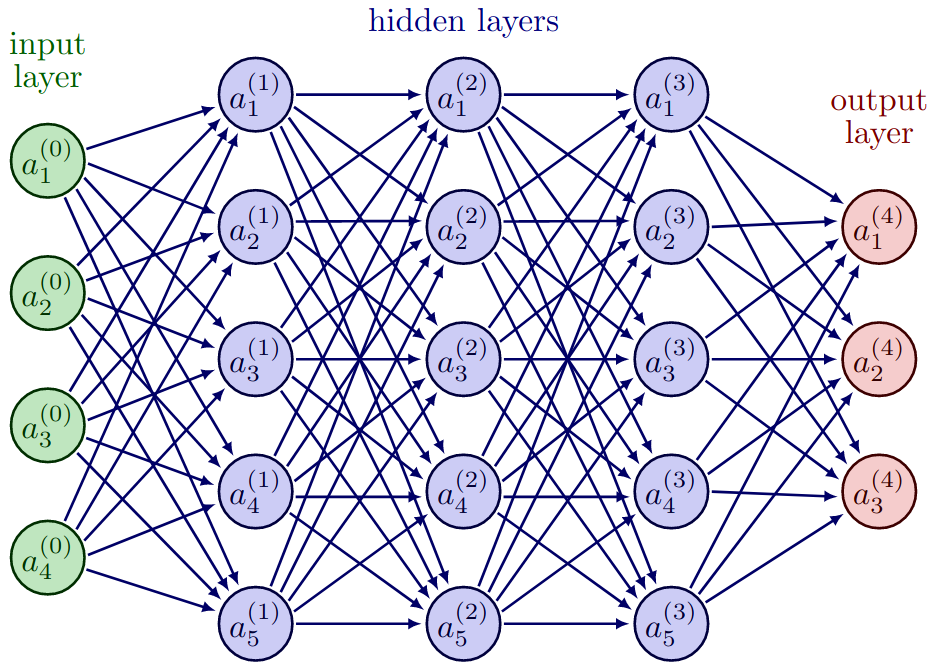
\includegraphics[width=0.7\columnwidth]{resources/chapter3/mlp.png}
		\caption{Illustration of model with a multi-layer perceptron. \cite{tikz_neural_networks}}
		\label{fig:Multilayer Perceptron}
	\end{figure}
	
	\subsection{Convolutional Neural Networks (CNNs)}
	Convolutional neural networks (CNNs) are a type of artificial neural network specifically designed for image recognition and processing. They are inspired by the structure of the visual cortex in animals, which is arranged in such a way as to be sensitive to specific patterns or features in visual stimuli.
	
	CNNs are composed of multiple layers of artificial neurons, or ``perceptrons," arranged in a three-dimensional structure, with the input layer at the bottom, followed by one or more hidden layers, and an output layer at the top. The hidden layers are made up of multiple ``convolutional" layers, which apply a set of learnable filters to the input data and produce a set of feature maps. These feature maps are then processed by one or more ``pooling" layers, which downsample the data and reduce the spatial resolution of the feature maps. Finally, the output of the pooling layers can be passed through a fully connected layer, which produces the final output of the CNN.
	
	CNNs are trained using a variant of the backpropagation algorithm, in which the weights of the filters and connections between the neurons are adjusted based on the error between the predicted output and the actual output. This process is repeated until the error is minimized and the CNN is able to accurately classify or predict the output for a given input.
	
	\begin{figure}[h!]
		\centering
		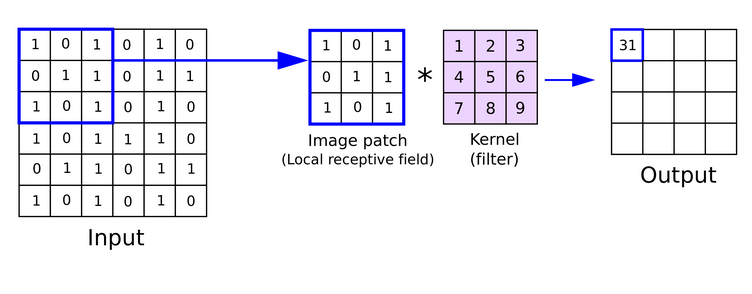
\includegraphics[width=0.7\columnwidth]{resources/chapter3/cnn2.png}
		\caption{Illustration of working of Convolutional Neural Networks (CNNs). \cite{reynolds2023convolutional}}
		\label{fig:CNN2}
	\end{figure}
	
	CNNs have achieved state-of-the-art results in many image recognition tasks and are widely used in applications such as object detection, image classification, and facial recognition.
	
	\subsection{Elements of Neural Network}
	\subsubsection{Activation function}
	
	Activation functions are used to adjust the output of each layer in a neural network. There are two types: linear and non-linear. Linear activation functions are not commonly used. Instead, non-linear activation functions are used to introduce non-linearities to the network, allowing it to learn non-linear relationships between inputs and outputs. Some common non-linear activation functions include sigmoid, tanh, ReLU, and leaky ReLU. The graphs of these activation functions are shown in Figure \ref{fig:Activation_functions} \cite{image2023, szandala2021review}.
	
	\begin{figure}[h!]
		\centering
		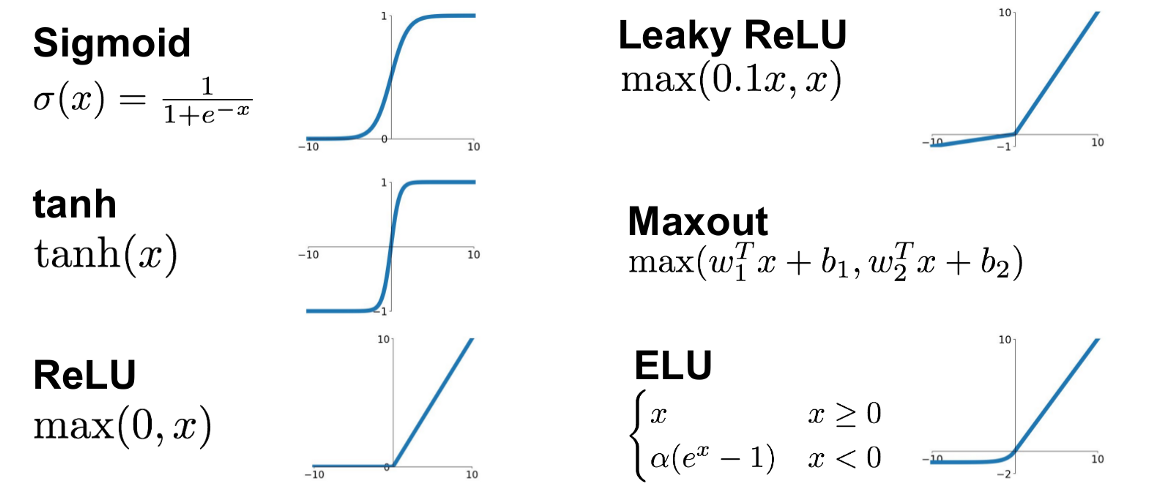
\includegraphics[width=100mm]{resources/chapter3/activation_functions.png}
		\caption{Activation functions}
		\label{fig:Activation_functions}
	\end{figure}
	
	\subsubsection{Loss function}
	
	A Loss function is used to check how our model compares to an ideal model. There are many types of loss functions, one of which can be selected based on the problem being solved. The most common ones for regression are mean absolute error (MAE) also referred to as L1 loss, mean squared error (MSE) also referred to as L2 loss. The most common ones for classification problems are binary cross-entropy (BCE) loss and hinge loss \cite{wang2020comprehensive}. And others include Normalized Cross-Correlation and mutual information loss to measure the similarity between the two images. A typical loss function plotted against the number of epochs is given in the Figure \ref{fig:LossFun} \cite{image2023mse}. 
	
	\begin{figure}[h!]
		\centering
		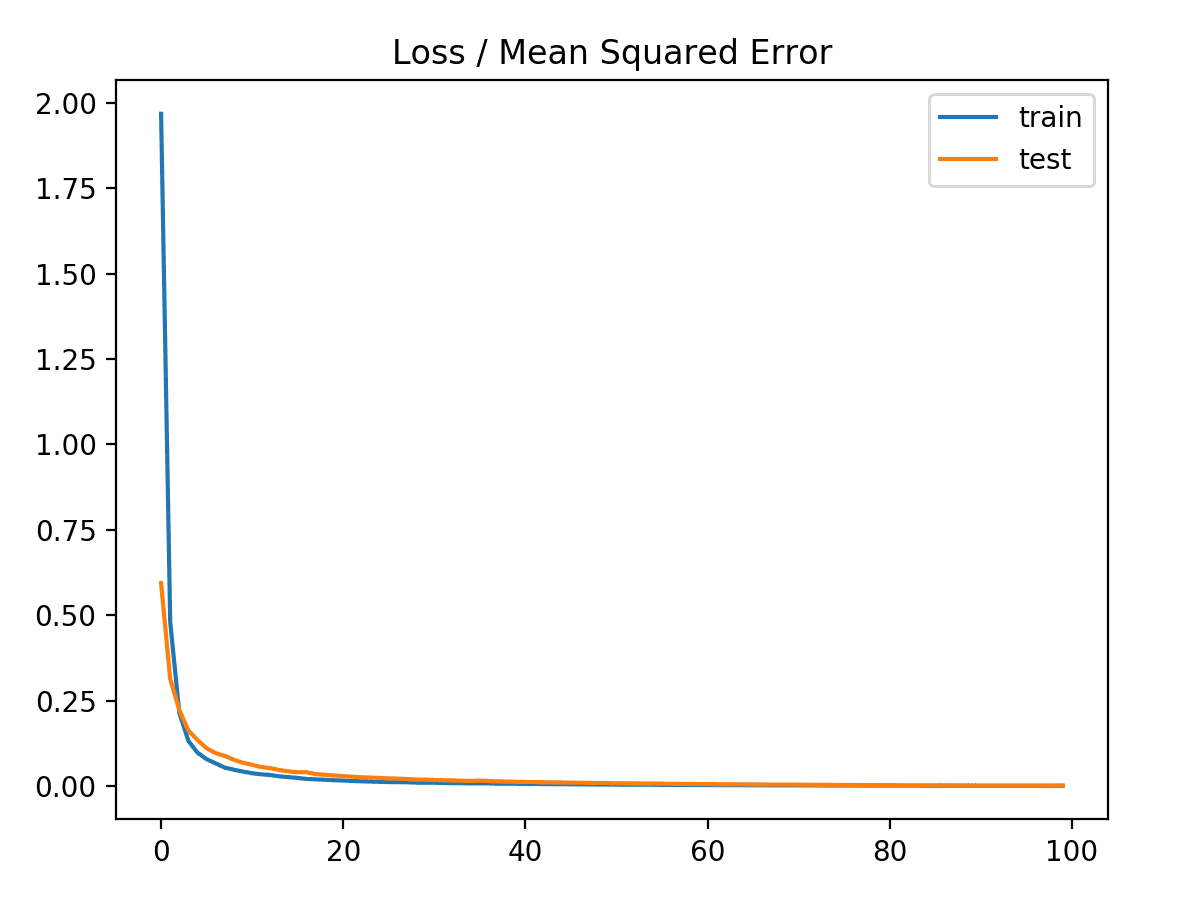
\includegraphics[scale=0.2]{resources/chapter3/lossfun.png}
		\caption{Loss function}
		\label{fig:LossFun}
	\end{figure}
	
	\subsubsection{Backpropagation}
	
	Backpropagation is an algorithm used to train artificial neural networks. It involves using gradient descent to propagate the error computed by the loss function backwards through the network. The gradients of the error with respect to the model's parameters are calculated using the chain rule of calculus, and these gradients are used to update the parameters of the model.
	
	\subsubsection{Learning rate}
	
	The learning rate is a hyperparameter that determines the size of the updates made to the model's weights during training. It is important to choose an optimal learning rate, as a value that is too small can cause the training process to be slow and potentially get stuck, while a value that is too large can cause the training process to be unstable and result in sub-optimal learned parameters. The learning rate can also be scheduled to change during the training process. \cite{senior2013empirical}. 
	
	
	\subsubsection{Optimizer}
	
	Optimizers are important in the training process of a model, as they use the gradients computed through backpropagation to update the model's parameters and minimize the loss. Some common optimizers include Adam and stochastic gradient descent. Research has shown that the Adam algorithm tends to perform well in most cases \cite{zaheer2019study}.
	
	\subsection{Encoder-Decoder Architecture}
	The encoder-decoder architecture is a type of neural network architecture commonly used in natural language processing and machine translation tasks. It consists of two main components: an encoder and a decoder.
	\begin{enumerate}
		\item The encoder takes in a sequence of input data, such as a sentence in a source language, and converts it into a fixed-length internal representation, called a ``latent representation" or ``latent vector." This latent vector captures the meaning of the input sequence and is typically much smaller in size than the input sequence itself.
		\item The decoder takes the latent vector as input and generates an output sequence, such as a translation of the input sentence into a target language. The decoder is typically trained to generate the output sequence by predicting the next word in the sequence based on the previous words and the latent vector.
	\end{enumerate}
	
	The encoder-decoder architecture has been widely used in natural language processing tasks, such as machine translation, language modeling, and text summarization. It has also been applied to other domains, such as image generation and sequence-to-sequence modeling in time series data.
	
	\begin{figure}[h!]
		\centering
		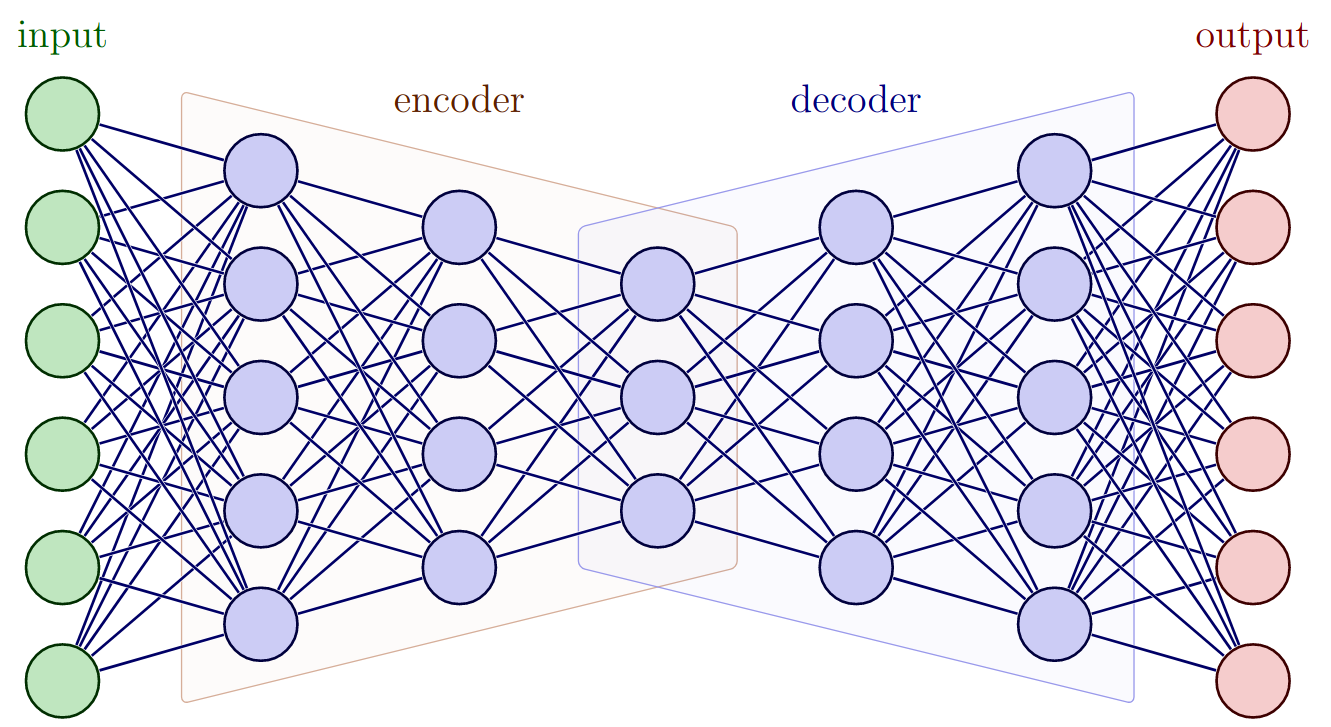
\includegraphics[width=0.7\columnwidth]{resources/chapter3/encoderdecoder.png}
		\caption{Illustration of encoder decoder architecture \cite{tikz_neural_networks}.}
		\label{fig:Encoder Decoder architecture}
	\end{figure}
	
	In image processing, the encoder-decoder architecture can be used to perform tasks such as image compression and image reconstruction.	In image compression, the encoder takes in an input image and compresses it into a smaller representation, called a ``latent representation" or ``latent vector" that captures the important features of the image. This latent vector captures the important features of the input image and is typically much smaller in size than the input image itself. The decoder takes the latent vector as input and reconstructs an output image that is as close as possible to the original input image.
	
	In image reconstruction tasks, the encoder-decoder architecture can be used to restore images that have been damaged or degraded in some way, such as by noise, blur, or missing pixels. It can also be used to perform tasks such as super-resolution, in which a low-resolution image is upscaled to a higher resolution.
	
	\subsection{U-Net}\label{subsec:unet}
	U-Net is a convolutional neural network (CNN) architecture designed for image segmentation tasks. It was developed by Olaf Ronneberger, Philipp Fischer, and Thomas Brox in 2015 \cite{UNet} and has since become a widely used model for image segmentation in medical imaging and other domains. U-Net is typically trained using supervised learning, with the goal of minimizing the error between the predicted output segmentation map and the ground truth segmentation map. It has been widely used in medical imaging tasks, such as tumor segmentation and organ segmentation, and has also been applied to other domains, such as satellite image analysis and surface defect detection.
	
	\begin{figure}[h!]
		\centering
		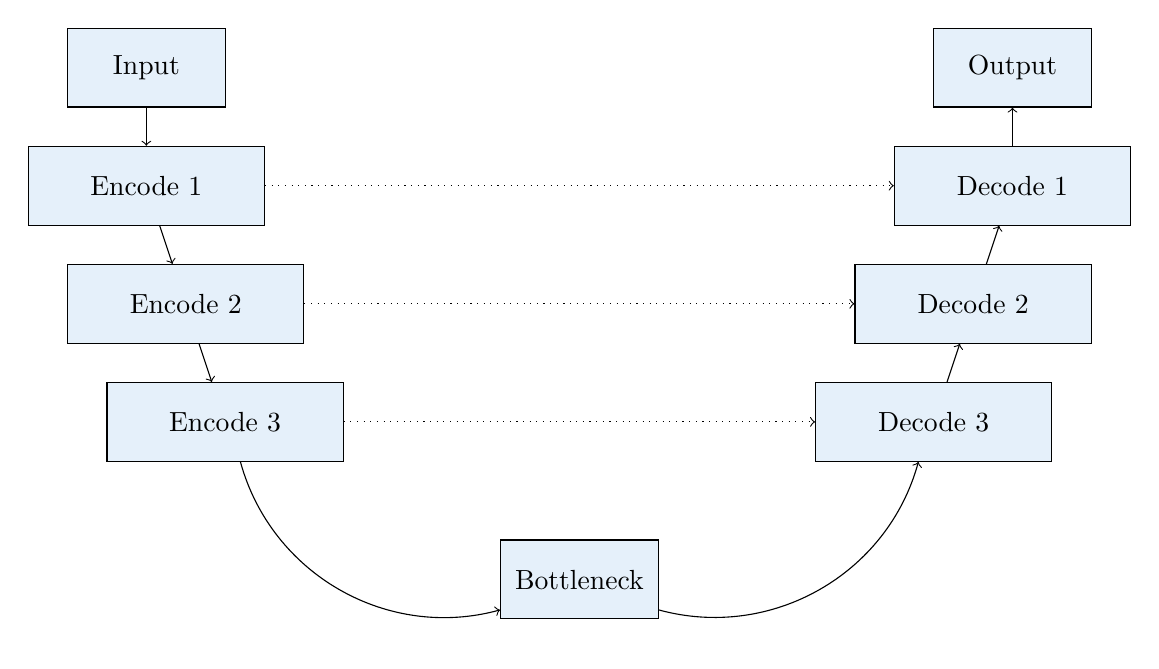
\begin{tikzpicture}[node distance=1.5cm]
		
		% Draw the input layer
		\node (input) [draw, fill=rwth-blue-5, minimum width=2cm, minimum height=1cm] {Input};
		
		% Draw the first downsampling layer
		\node (encode1) [draw, fill=rwth-blue-5, minimum width=3cm, minimum height=1cm, below of=input] {Encode 1};
		
		% Draw the second downsampling layer
		\node (encode2) [draw, fill=rwth-blue-5, minimum width=3cm, minimum height=1cm, below of=encode1, xshift=0.5cm] {Encode 2};
		
		% Draw the third downsampling layer
		\node (encode3) [draw, fill=rwth-blue-5, minimum width=3cm, minimum height=1cm, below of=encode2, xshift=0.5cm] {Encode 3};
		
		% Draw the first bottleneck layer
		\node (bottleneck) [draw, fill=rwth-blue-5, minimum width=2cm, minimum height=1cm, right of=encode3, xshift=3cm, yshift=-2cm] {Bottleneck};
		
		% Draw the upsampling layers
		\node (decode3) [draw, fill=rwth-blue-5, minimum width=3cm, minimum height=1cm, right of=bottleneck, xshift=3cm, yshift=2cm] {Decode 3};
		\node (decode2) [draw, fill=rwth-blue-5, minimum width=3cm, minimum height=1cm, above of=decode3, xshift=0.5cm] {Decode 2};
		\node (decode1) [draw, fill=rwth-blue-5, minimum width=3cm, minimum height=1cm, above of=decode2, xshift=0.5cm] {Decode 1};
		
		% Draw the output layer
		\node (output) [draw, fill=rwth-blue-5, minimum width=2cm, minimum height=1cm, above of=decode1] {Output};
		
		% Connect the layers with arrows
		\draw[->] (input) -- (encode1);
		\draw[->] (encode1) -- (encode2);
		\draw[->] (encode2) -- (encode3);
		\draw[->] (encode3) to[bend right=45] (bottleneck);
		\draw[->] (bottleneck) to[bend right=45] (decode3);
		\draw[->] (decode3) -- (decode2);
		\draw[->] (decode2) -- (decode1);
		\draw[->] (decode1) -- (output);
		
		% Add skip connections
		\draw[dotted,->] (encode1) -- (decode1);
		\draw[dotted,->] (encode2) -- (decode2);
		\draw[dotted,->] (encode3) -- (decode3);	
		\end{tikzpicture}
		\caption{A graphical representation of the U-Net model.}
		\label{fig:unet_tikzpicture}
	\end{figure}
	Figure~\ref{fig:unet_tikzpicture} shows the structure of the U-Net model. The model has two main parts: an encoder that reduces the spatial resolution of the input image and increases the number of feature maps, and a decoder that does the opposite. The encoder uses convolutional layers with a stride of 2 to downsample the input image, and the decoder uses transposed convolutional layers to upsample the feature maps. The bottleneck layer connects the encoder and decoder and acts as a bridge between them. It allows the decoder to use the high-level features extracted by the encoder to generate a detailed segmentation map. The model also has skip connections, shown as dotted lines in the figure, that allow the decoder to access the features extracted by the encoder at each level of the network. This helps the model to use both high-level and low-level features and preserves spatial information, leading to more accurate segmentation results.
	
	The input to the model is an image and the output is a segmentation mask, with each pixel in the mask corresponding to a particular class in the image. The U-Net model is commonly used in medical imaging, where it can be trained to segment organs or other structures in images.
	
	\chapter{Implementations and Data Preparation}\label{chap:imp_and_data}
	In the chapter~\nameref{chap:litreture}, we discussed various traditional and deep learning approaches for medical image registration. In this chapter, we will address the research design and introduce concepts that are highly relevant to the methods used in this thesis.
	
	In the following three sections, we will address the specifics of the Voxelmorph architecture \cite{Balakrishnan_2019} that served as the foundation for our study, explore the concept of landmark points and their importance in the field of image registration, and provide an overview of the dataset we used and the preprocessing steps we applied to it in order to prepare it for analysis.
	
	\section{The Voxelmorph Architecture: An Overview}
	\label{sec:vxm_architecture}
	
	In the paper, ``VoxelMorph: A Learning Framework for Deformable Medical Image Registration," \cite{Balakrishnan_2019} the authors introduced a deep learning architecture called Voxelmorph for medical image registration. The architecture of Voxelmorph is designed specifically for medical image registration, which is the process of aligning two or more medical images of the same subject, taken at different times or using different modalities, in order to compare and analyze them.
	
	The Voxelmorph architecture consists of two main components: an encoder-decoder CNN architecture (U-Net) \cite{UNet} and a spatial transformer network (STN) \cite{NIPS2015_33ceb07b}. The U-Net is responsible for learning the spatial transformations needed to align the images, while the spatial transformer network is responsible for applying those transformations to the images.
	
	In the Voxelmorph architecture, the U-Net is modified to predict a dense displacement field, which describes how the pixels in the target image should be displaced in order to align with the source image. The displacement field is then passed through spatial transformer network (STN), which uses it to warp the moving image and bring it into alignment with the fixed image. The U-Net architecture is particularly well-suited for this task because it is able to capture both high-level semantic features and fine-grained spatial details in the input images.
	
	\begin{figure}[h!]
		\centering
		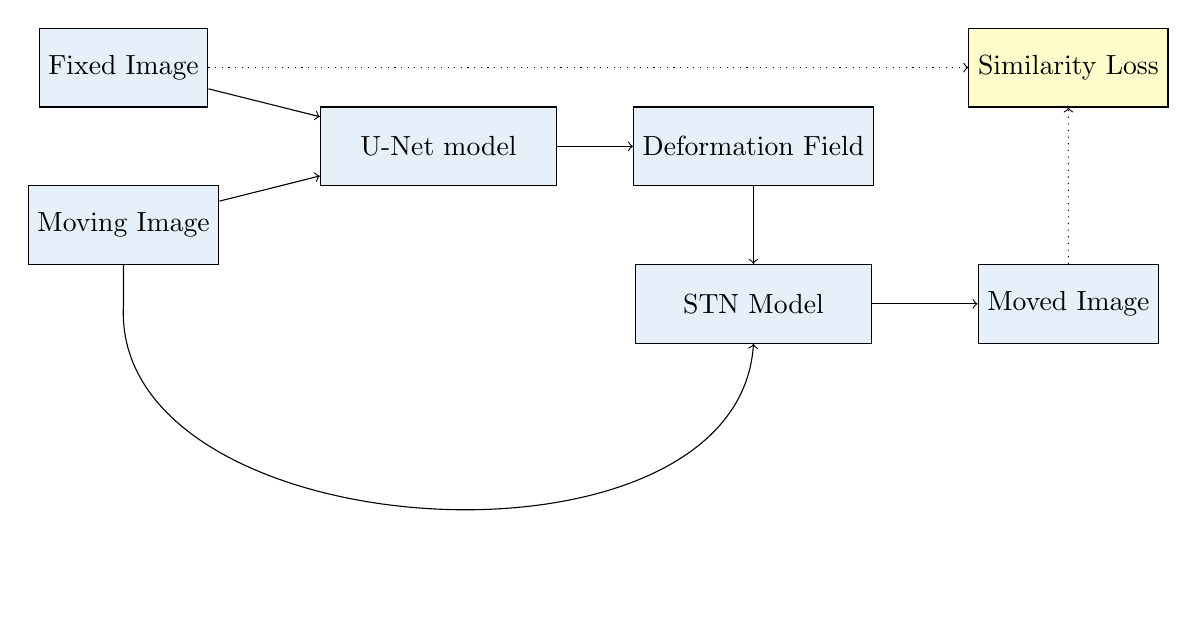
\begin{tikzpicture}[node distance=2cm]
		% Draw the input layer
		\node (fixed) [draw, fill=rwth-blue-5, minimum width=2cm, minimum height=1cm] {Fixed Image};
		\node (moving) [draw, fill=rwth-blue-5, minimum width=2cm, minimum height=1cm, below of=fixed] {Moving Image};
		
		% Draw the U-Net model
		\node (unet) [draw, fill=rwth-blue-5, minimum width=3cm, minimum height=1cm, right of=fixed, xshift=2cm, yshift=-1cm] {U-Net model};
		
		% Draw the output of the U-Net model
		\node (deformation) [draw, fill=rwth-blue-5, minimum width=2cm, minimum height=1cm, right of=unet, xshift=2cm] {Deformation Field};
		
		% Draw the STN model
		\node (stn) [draw, fill=rwth-blue-5, minimum width=3cm, minimum height=1cm, below of=deformation] {STN Model};
		
		% Draw the output of the STN model
		\node (moved) [draw, fill=rwth-blue-5, minimum width=2cm, minimum height=1cm, right of=stn, xshift=2cm] {Moved Image};
		
		% Draw the similarity loss block
		\node (loss) [draw, fill=yellow!20, minimum width=2cm, minimum height=1cm, right of=fixed, xshift=10cm] {Similarity Loss};
		
		% Connect the layers with arrows
		\draw[->] (fixed) -- (unet);
		\draw[->] (moving) -- (unet);
		\draw[->] (unet) -- (deformation);
		\draw[->] (deformation) -- (stn);
		\draw[->] (moving) -- (moving |- stn) to[bend right=90] (stn);
		\draw[->] (stn) -- (moved);
		
		% Draw the arrows between the blocks
		\draw[dotted, ->] (fixed) -- (loss);
		\draw[dotted, ->] (moved) -- (loss);	
		\end{tikzpicture}
		\caption{Graphical representation of the Voxelmorph model showing the use of a U-Net model to take in the fixed and moving images as input and produce a deformation field as output.}
		\label{fig:vxm_tikzpicture}
	\end{figure}
	
	The basic structure of Voxelmorph consists of an encoder-decoder architecture (U-Net) with skip connections between the encoder and decoder layers as illustrated in subsection~\ref{subsec:unet} on page~\pageref{subsec:unet}. The encoder takes in a pair of input images and extracts features from them, while the decoder generates a dense displacement field that maps pixels from one image to the other. The skip connections allow the decoder to access the features extracted by the encoder at each level of the network, which helps to preserve spatial information and improve the accuracy of the displacement field.
	
	Figure~\ref{fig:vxm_tikzpicture} is an illustration of the Voxelmorph model. The model consists of two main components: a U-Net model and an STN model. The U-Net model takes as input the fixed image and the moving image, and produces a deformation field as output. The STN model, or spatial transformer network model, takes as input the deformation field and the moving image, and produces a moved image as output. The STN model is responsible for applying the deformation field to the moving image, effectively aligning it with the fixed image. The moved image is then compared to the fixed image using a similarity loss function, which is represented by the block labeled ``Similarity Loss" in the illustration. The dotted arrows in the illustration indicate that the similarity loss is calculated between the fixed image and the moved image. The model is trained to minimize the similarity loss, which helps to align the moving image with the fixed image.
	
	Figure~\ref{fig:vxmaux_tikzpicture} depicts a model that includes an auxiliary information block in addition to the fixed and moving images as input to the U-Net model. This auxiliary information can improve the accuracy of the deformation field produced by the U-Net model. Researchers have found that using segmentation masks as auxiliary input can enhance the model's performance on specific tasks. For example, segmentation masks can help the model focus on specific areas of the image, such as the brain or heart, and improve the accuracy of the displacement field in those areas.
	
	The Voxelmorph architecture is designed to be fast and accurate, and it has been widely used in the field of medical image analysis since its introduction. Considering its impressive performance and widespread adoption in the field of medical image analysis, we decided to use it in our research as the base architecture.
	
	\begin{figure}[h!]
		\centering
		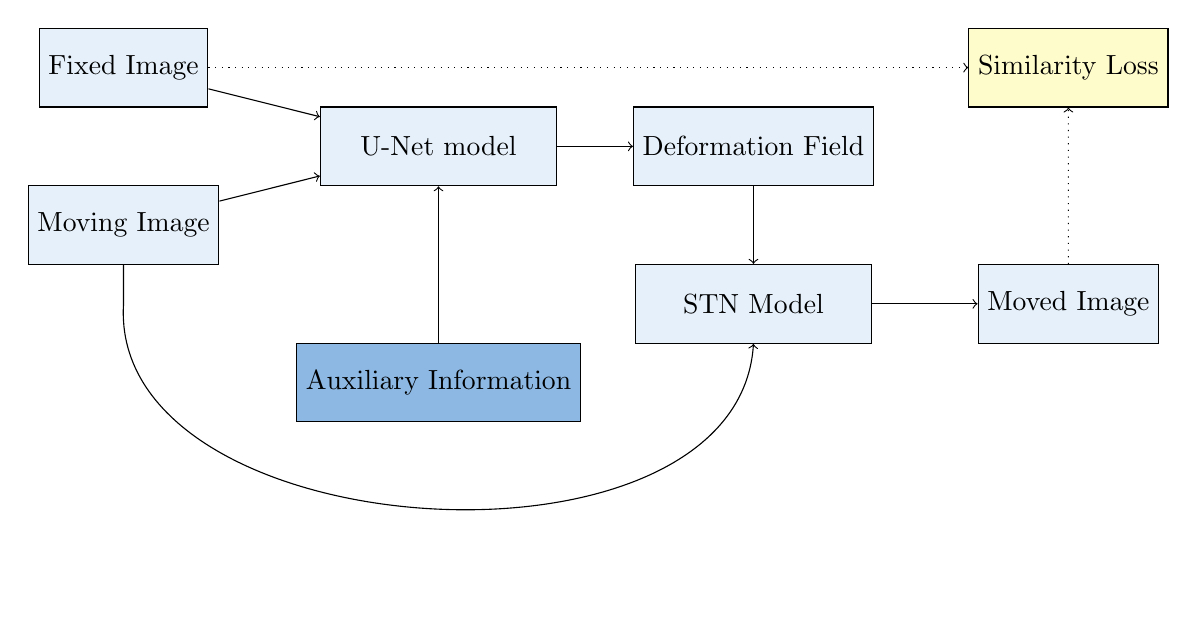
\begin{tikzpicture}[node distance=2cm]
		% Draw the input layer
		\node (fixed) [draw, fill=rwth-blue-5, minimum width=2cm, minimum height=1cm] {Fixed Image};
		\node (moving) [draw, fill=rwth-blue-5, minimum width=2cm, minimum height=1cm, below of=fixed] {Moving Image};
		
		% Draw the U-Net model
		\node (unet) [draw, fill=rwth-blue-5, minimum width=3cm, minimum height=1cm, right of=fixed, xshift=2cm, yshift=-1cm] {U-Net model};
		
		% Draw the aux
		\node (auxinfo) [draw, fill=rwth-blue-3, minimum width=2cm, minimum height=1cm, below of=unet, yshift=-1cm] {Auxiliary Information};
		
		% Draw the output of the U-Net model
		\node (deformation) [draw, fill=rwth-blue-5, minimum width=2cm, minimum height=1cm, right of=unet, xshift=2cm] {Deformation Field};
		
		% Draw the STN model
		\node (stn) [draw, fill=rwth-blue-5, minimum width=3cm, minimum height=1cm, below of=deformation] {STN Model};
		
		% Draw the output of the STN model
		\node (moved) [draw, fill=rwth-blue-5, minimum width=2cm, minimum height=1cm, right of=stn, xshift=2cm] {Moved Image};
		
		% Draw the similarity loss block
		\node (loss) [draw, fill=yellow!20, minimum width=2cm, minimum height=1cm, right of=fixed, xshift=10cm] {Similarity Loss};
		
		% Connect the layers with arrows
		\draw[->] (fixed) -- (unet);
		\draw[->] (moving) -- (unet);
		\draw[->] (unet) -- (deformation);
		\draw[->] (auxinfo) -- (unet);
		\draw[->] (deformation) -- (stn);
		\draw[->] (moving) -- (moving |- stn) to[bend right=90] (stn);
		\draw[->] (stn) -- (moved);
		
		% Draw the arrows between the blocks
		\draw[dotted, ->] (fixed) -- (loss);
		\draw[dotted, ->] (moved) -- (loss);	
		\end{tikzpicture}
		\caption{Graphical representation of the Voxelmorph model with auxiliary information input, showing how in addition to the fixed and moving images, the auxiliary information is also provided as input to the U-Net model to produce a deformation field as output.}
		\label{fig:vxmaux_tikzpicture}
	\end{figure}
	
	\section{Landmark Points: A Key Element in Image Registration} \label{sec:landmark_points}
	Landmark points in image registration are points of reference in an image that are used to align or register two or more images. These points are often selected based on their distinct and easily identifiable features, and are used to establish a common coordinate system for the images being registered.
	
	The term ``gold standard" refers to the fact that these points are considered to be the most accurate and reliable points of reference for aligning images. This term is used metaphorically, as gold is often considered a symbol of excellence and high quality. In the context of image registration, the use of landmark points as the gold standard for alignment helps to ensure the accuracy and reliability of the registration process.
	
	In \textit{larvalign} \cite{larvalign}, biologists identified 30 potential landmarks in brain scans of Drosophila larvae. The same landmarks are used in this work. The xy positions of all 30 landmarks used can be seen in the Figure~\ref{fig:landmark_annotations}, which is a direct adaptation from the \emph{larvalign} paper \cite{larvalign}. The names of each landmark can be found in Table 1 of \emph{larvalign} paper \cite{larvalign}.
	
	\begin{figure}[h!]
		\centering
		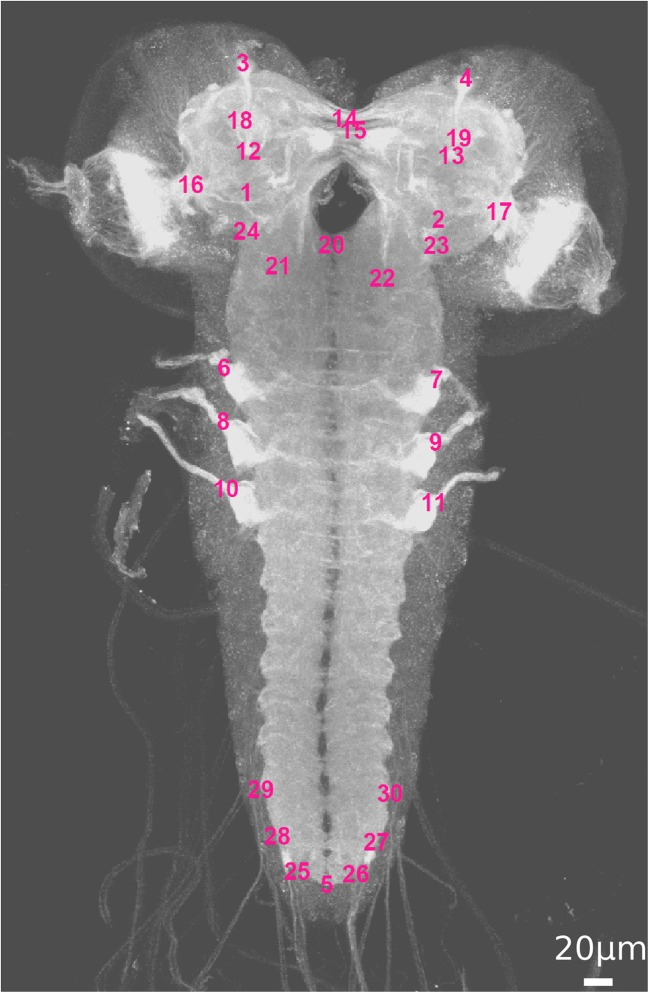
\includegraphics[width=0.5\columnwidth]{resources/chapter3/landmarks.jpg}
		\caption{Maximum Intensity Projection (MIP) of a brain scan of a larval specimen showing annotated landmarks as per the method described in \textit{larvalign}. \cite{larvalign}}
		\label{fig:landmark_annotations}
	\end{figure}
	
	To annotate or label these landmark points in the brain scan images, we can use ImageJ software. ImageJ is an open-source image processing software that offers ``Point Tool" to label the landmark points. The ``Point Tool" allows you to place a single point on an image by clicking on the desired location.
	
	To use the ``Point Tool" in ImageJ Fiji for landmark annotation, follow these steps:
	\begin{enumerate}
		\item Open the image you want to annotate in ImageJ Fiji.
		\item Click on the ``Point Tool" icon in the toolbar at the top of the window. This will activate the tool and allow you to place points on the image.
		\item Click on the location in the image where you want to place a point. A small crosshair will appear at the location you clicked.
		\item Use the ``Set/Add Point" button to label the point with a name or identifier. You can enter the name in the text field that appears and then click ``OK" to set the name for the point.
		\item Repeat steps 3 and 4 for each additional point you want to place on the image.
		\item When you are finished annotating the points, you can use the ``Point Tool" icon again to deactivate the tool and return to the default cursor.
	\end{enumerate}

	When you use the ``Point Tool" to annotate an image in ImageJ, the result of the annotation will be saved in the same directory as the image as an XML file with a ``.points" extension. This file will contain the coordinates of the points that you added to the image, as well as any other information about the points (such as labels and attributes).
	
	\section{Data Preparation: Selecting and Preprocessing Datasets}
	This section covers the selection and preparation of datasets for use with the Voxelmorph model. It will cover how to categorize the datasets for training and testing, as well as the necessary preprocessing steps to ensure that the data is properly formatted for the model.
	
	\subsection{Dataset}
	For this research, we have obtained three datasets from different sources: the \texttt{Leipzig dataset} from the University of Leipzig in Germany, the \texttt{Janelia dataset} from the Janelia Research Campus in Virginia, and the \texttt{Larvalign dataset} from the \textit{larvalign} research paper \cite{larvalign}. These datasets will be referred to by these names throughout the study.
	
	As shown in Table~\ref{tab:mytable}, each dataset for this study was divided by the biologists into three categories: good quality, medium quality, and random quality. This subdivision was necessary to ensure that the training data were balanced and to evaluate the performance of the model at different levels of image quality.
	
	% Please add the following required packages to your document preamble:
	\begin{table}[h!]
		\centering
		\resizebox{\textwidth}{!}{%
			\begin{tabular}{|l|l|c|c|c|}
				\hline
				& Quality & Number of Scans & Original Resolution & Scaled Resolution           \\ \hline
				\multirow{3}{*}{\texttt{Leipzig dataset}}& - & 100             & 980x1440x81         & \multirow{9}{*}{256x512x64} \\ \cline{2-3}
				& - & 052              & 512x512x104         &                             \\ \cline{2-3}
				& - & 200             & 592x800x102         &                             \\ \cline{1-3}
				\multirow{3}{*}{\texttt{Janelia dataset}}                      & Medium & 200             & 977x1428x76         &                             \\ \cline{2-3}
				& Good & 200             & 981x1428x76         &                             \\ \cline{2-3}
				& Random & 200             & 973x1434x79         &                             \\ \cline{1-3}
				\multirow{3}{*}{\texttt{Larvalign dataset (Test Data)}}                        & Medium & 021              & 973x1434x79         &                             \\ \cline{2-3}
				& Good & 020              & 981x1430x79         &                             \\ \cline{2-3}
				& Random & 025              & 977x1432x77         &                             \\ \hline
			\end{tabular}
		}
		\caption{Dataset distribution.}
		\label{tab:mytable}
	\end{table}
	
	One problem that arose during data preparation was that the images had different sizes. In order to input the images into the network, they had to be resized to a uniform size. In addition, the Voxelmorph model is computationally intensive and requires a significant amount of memory due to the different encoding layers and the need to keep encoded feature maps for later use in the decoding phase by skip connections. Experiments showed that using the model with images of size \texttt{256x512x64} required at least \texttt{16GB GPU}. If the image volumes were larger than this resolution, a GPU with a memory capacity proportional to the increase in the size of the input images was required. Empirically, it was found that the memory requirements of the GPU were directly proportional to the increase in image volume by more than 1. Therefore, it was decided to use images with a reduced resolution of \texttt{256x512x64} for all experiments. Unless otherwise stated, all experiments from this point forward are based on images at this resolution, and all results reported are also at this resolution. The downscaling was done by resampling the image using the bicubic interpolation algorithm included in the ImageJ Fiji tool.
	
	\subsection{Extracting registration channel from the scans}
	
	Brain scans were provided to us in the form of LSM files. These LSM Image files are used to store multi-channel, multi-slice, and time series image data generated by the microscope. The LSM file format includes both image data and metadata, including information about the microscope settings and the image acquisition process. They can be opened and viewed using specialized software such as ImageJ or the LSM File Toolbox in MATLAB, which can read the metadata and display the image data.
	
	Accordingly, in our case, there were three channels: one containing neuropil (NP) staining, one containing nerve tract (NT) staining, and one containing gene expression (GE). The NP channel is used for registration and thus is also called as registration channel, but the order of the channels was not fixed. In the \texttt{Janelia dataset}, the NP channel was always in the third channel, but in the \texttt{Leipzig dataset}, it could have been in either the second or third channel, as informed by neurobiologists. To automatically identify the NP channel, the metadata of the images needed to be read and the ``IlluminationChannel Wavelength" or ``IlluminationChannel Name" tags had to be checked for a value of 633. This could be done using the ``LSM File Toolbox" in MATLAB, which provided functions for reading LSM files. Figure~\ref{fig:lsmtoolbox} shows how to extract metadata from LSM Image files to read the ``IlluminationChannel Wavelength" or ``IlluminationChannel Name" tags. 
	
	\begin{figure}[h!]
		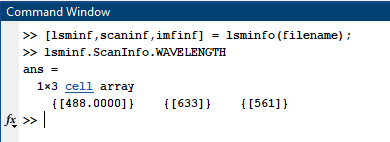
\includegraphics[width=0.5\columnwidth]{resources/chapter4/lsmtoolbox.png}
		\caption{Using the LSM Toolbox in MATLAB to read and extract metadata from LSM image files.}
		\label{fig:lsmtoolbox}
	\end{figure}

	Out of the three channels present in the brain scans, only the channel containing neuropil staining was used for the purpose of training or prediction using deep neural network. The other two channels, containing nerve tract staining and gene expression data, were not used for registration.
	
	\subsection{Affine registration}
	According to the Voxelmorph research paper \cite{Balakrishnan_2019}, it is recommended to affine align the input images before using them with the Voxelmorph model for deformable registration. This preprocessing step could improve the performance of the model compared to using the images without affine alignment.
	
	Similar to Voxelmorph, the \textit{larvalign} \cite{larvalign} software also performed affine alignment and then applied non-rigid registration to the affine-aligned image. Therefore, to compare the efficiency of non-rigid registration using \textit{larvalign} versus a deep learning method, it was decided to use \textit{larvalign} to perform affine registration on the input images so that both approaches would work on the same preprocessed data. This allowed for a fair comparison between the two approaches.
	
	\begin{tcolorbox}[colback=rwth-blue-5,colframe=rwth-blue-1,title=\textbf{\textit{larvalign} Software}]
		textit{larvalign} is based on the Elastix Registration Toolbox, which is a widely used, open-source medical image registration toolbox that allows for both rigid and non-rigid registration of medical images such as CT, MRI, and PET scans.
		\tcblower
		Elastix uses optimization algorithms to minimize a cost function that measures the difference between the images and finds the transformation that best aligns them. It offers a range of customization options, including the choice of optimization algorithm, cost function, and regularization terms, as well as pre-processing and post-processing tools to improve the accuracy and efficiency of the registration.
	\end{tcolorbox}
	
	Figure~\ref{fig:affine_larvalign} illustrates an example of an image before and after affine alignment.
	
	\begin{figure}[h!]
		\centering
		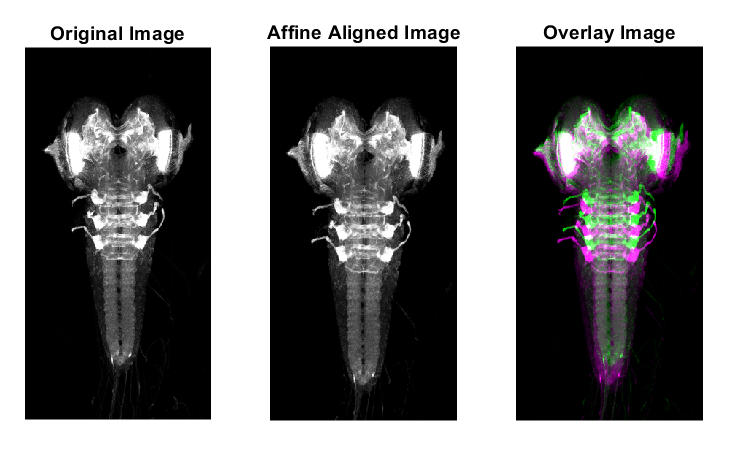
\includegraphics[width=0.7\columnwidth]{resources/chapter3/np_58E02_37E10_MB299C_021713A_scaled.tif.png}
		\caption{The effect of affine alignment on image registration. The left plot shows the original unregistered image, the center plot shows the image after affine registration using the \textit{larvalign} method \cite{larvalign}, and the right plot shows the overlay of the affine-registered image and the original image.}
		\label{fig:affine_larvalign}
	\end{figure}

	Affine alignment is a method for aligning two images by applying an affine transformation to one of the images. An affine transformation can include rotation, scaling, translation, and shearing, and it can be used to match corresponding points in the two images. It is possible that the scale of the moving image could be changed during affine registration to match the scale of the fixed image so that moving image is aligned as much as possible with the fixed image. In the Figure~\ref{fig:affine_larvalign}, the affine registration is performed against the \textit{larvalign} template (shown in Figure~\ref{fig:Registration} on page~\pageref{fig:Registration}), and the resulting alignment is shown before and after registration in the left and center images, respectively. The right image shows an overlay of the two images, before and after registration.
	
	\subsection{Background Noise Removal and Normalizing}
	Background noise removal and normalizing the data are important pre-processing steps in deep learning because they can improve the performance and accuracy of the network. Removing background noise helps to eliminate irrelevant information from the input data, making it easier for the network to focus on the important features. Normalizing the data is important because it helps to ensure that all input features are on the same scale. In the following two subsections, we will discuss more about these.
	\subsubsection{Background Noise Removal}
	To prepare the image for further processing, the noise in the background was removed by clipping the intensity values of the pixels between the mean intensity of the image and the maximum intensity (\texttt{255 for an 8-bit image}). Any values that are below the mean intensity are set to zero, while values above the mean intensity are retained. This helped to clean up the image and reduce the impact of noise on subsequent steps.
	
	The below pseudo code defines a function called \texttt{cleanup\_background} that takes an image as input and returns a modified version of the image with the background pixels set to zero.
	
	\begin{lstlisting}[language=python, label=lst:bgcorrection, caption=Pseudo function to show the background noise removal in an image.]

	def cleanup_background(image):
		# Find the mean intensity of the image
		mean_intensity = find_mean_intensity(image)
	
		# Set the low and high values for clipping
		low = mean_intensity
		high = 255
	
		# Clip the pixel intensity values between the low and high values
		image = clip_intensity_values(image, low, high)
	
		# Set the low clipped values to zero
		image = set_low_values_to_zero(image, low)
	
		return image
	
	\end{lstlisting}	
	
	The function shown in the Listing~\ref{lst:bgcorrection} performs the following steps:
	
	\begin{enumerate}
		\item It calls a function called \texttt{find\_mean\_intensity} to calculate the mean intensity of the image.
		\item It sets the low and high values for clipping to the mean intensity and the maximum intensity (255), respectively.
		\item It calls a function called \texttt{clip\_intensity\_values} to clip the pixel intensity values between the low and high values. Any values below the low value are set to zero, while values above the low value are kept the same.
		\item It calls a function called \texttt{set\_low\_values\_to\_zero} to set the low clipped values to zero.
	\end{enumerate}
	
	\subsubsection{Normalizing the inputs}
	Normalizing the pixel values in the input images for use in a neural network could prevent problems such as vanishing or exploding gradients that could further impair the network's ability to learn effectively. One way to normalize the values is to scale them to be between 0 and 1, which can be achieved by dividing the pixel values by 255 (the maximum value for an 8-bit image). This approach was proposed by the authors of the Voxelmorph research paper because it was compatible with the leaky ReLU activation function used in the network, and so it was also used in this work. Other normalization techniques, such as subtracting the mean and dividing by the standard deviation of the pixel values, could also be used, but may not be as well suited for use with the Leaky ReLU function, as such normalization could result in negative values.
	
	The code for normalization is shown in Listing~\ref{lst:normalize}. This code defines a function called ``normalize" that takes a list of pixel values as input and returns a new list of normalized values. The pixel values are normalized by dividing each value by 255, the maximum value for a pixel in an 8-bit image.
	\newpage
	
	\begin{lstlisting}[language=python, label=lst:normalize, caption=Pseudo function to show the normalization of pixel intensity values.]
		def normalize(pixels):
			normalized_pixels = []
			for pixel in pixels:
				normalized_pixel = pixel / 255
				normalized_pixels.append(normalized_pixel)
			return normalized_pixels
	
		# Example usage
		pixels = [100, 150, 200, 50]
		normalized_pixels = normalize(pixels)
		print(normalized_pixels)  # Output: [0.39215686274509803, 0.5882352941176471, 0.7843137254901961, 0.19607843137254902]
	\end{lstlisting}
	
	
	
	\section{Loss Metric}\label{sec:loss_metric}
	A loss metric, also known as a loss function or objective function, is a measure of how well a machine learning model is able to predict the correct output for a given input. It is used to evaluate the performance of the model during training and to guide the optimization process.
	
	There are many different loss functions that can be used, depending on the specific task being addressed and the characteristics of the data. Some common loss functions that are used in image registration include:
	
	\begin{enumerate}
		\item \textbf{Mean squared error (MSE)}
		\item \textbf{Normalized cross-correlation (NCC)}
		\item \textbf{Landmark Registration Error (LRE)}
	\end{enumerate}
	
	\subsection{Mean squared error (MSE)}
	This is a common loss function that measures the average squared difference between the predicted output and the true output. It is often used for regression tasks and is particularly useful for image registration because it is sensitive to small errors and can effectively penalize large errors.
	
	The mean squared error (MSE) between two images, fixed image $I_f$ and moved image $I_m$, can be calculated as:
	
	$$ MSE = \frac{1}{n} \sum_{i=1}^n (I_f(i) - I_m(i))^2 $$
	
	where $n$ is the number of pixels in the images and $I_f(i)$ and $I_m(i)$ represent the intensity values of the fixed and moved images at pixel $i$, respectively.
	
	\subsection{Normalized cross-correlation (NCC)}
	This loss function measures the similarity between two images by calculating the cross-correlation between them and normalizing by the product of their standard deviations. It is commonly used in image registration because it is robust to intensity variations and can handle images with different scales or contrast.
	
	
	The normalized cross-correlation (NCC) between two images, fixed image $I_f$ and moved image $I_m$, can be calculated as:
	
	$$ NCC = \frac{\sum_{i=1}^n (I_f(i) - \mu_f)(I_m(i) - \mu_m)}{\sqrt{\sum_{i=1}^n (I_f(i) - \mu_f)^2}\sqrt{\sum_{i=1}^n (I_m(i) - \mu_m)^2}} $$
	
	where $n$ is the number of pixels in the images, $I_f(i)$ and $I_m(i)$ represent the intensity values of the fixed and moved images at pixel $i$, respectively, and $\mu_f$ and $\mu_m$ are the mean intensities of the fixed and moved images, respectively.
	
	\subsection{Landmark Registration Error (LRE)}
	This loss function measures the error between the predicted and true locations of landmarks in the images being registered. It is often used in conjunction with other loss functions to guide the optimization process and ensure that the images are correctly aligned.
	
	The landmark registration error between two images, fixed image $I_f$ and moved image $I_m$, can be calculated as the mean Euclidean distance between corresponding landmarks in the two images:
	
	$$ LRE = \frac{1}{K} \sum_{k=1}^K \sqrt{(x_f^k - x_m^k)^2 + (y_f^k - y_m^k)^2 + (z_f^k - z_m^k)^2} $$
	
	where $K$ is the number of landmarks, $(x_f^k, y_f^k, z_f^k)$ and $(x_m^k, y_m^k, z_m^k)$ represent the coordinates of the $k$-th landmark in the fixed and moved images, respectively.
	
	\section{Quality Assessment}\label{sec:quality}
	It is important to evaluate the performance of an image registration method using multiple metrics because the loss function, such as Normalized Cross-Correlation error (NCC) or Mean Squared Error (MSE), only measures the overall error in the registration. These metrics do not necessarily capture errors that occur at specific, biologically significant local regions. Therefore, evaluating the performance qualitatively and quantitatively becomes necessary to help to identify and quantify errors at such local regions. This can provide a more comprehensive assessment of the accuracy and effectiveness of the image registration method.
	
	\subsection{Quantitative Assessment} \label{subsec:quantitative}
	Quantitative assessment metrics are numerical measures that are used to evaluate the performance. The specific metric used will depend on the characteristics of the data and the goals of the analysis. In our image registration task, in addition to optimizing the loss function, such as Normalized Cross-Correlation error (NCC), we  evaluate below metrics to assess the performance of our approaches.
	\begin{enumerate}
		\item \textbf{VNC Terminal Error Indicator (VI)}
		\item \textbf{Thoracic Nerve Error Indicator (TI)}
		\item \textbf{Landmark Registration Error (LRE)}
	\end{enumerate}

	\subsubsection{VNC Terminal Error Indicator (VI)} \label{subsubsec:vi}
	To evaluate the accuracy of image registration in the ventral nerve cord (VNC) region, we consider two small 3D spherical volumes with a radius of 5 \textmu m at two terminal VNC positions defined in the fixed image and calculate the mutual information between the fixed and moving images in these spherical volumes. These two terminal positions chosen are the two landmark points - ``right A7 nerve entry point" and ``left A7 nerve entry point" in the fixed image. The original radius considered in \textit{larvalign}'s work \cite{larvalign} is 10 \textmu m. However, since we are now working with the downscaled images, 5 \textmu m was chosen so that the two spherical volumes do not overlap and just touch. Unlike in landmark registration error (LRE), the landmarks in this scenario only dictate the location of the region considered and does not contribute to the score in any other manner.
	
	A high score indicates that the image registration is good, while a low score indicates registration errors. Using this score, we can determine the quality of image registration at the tip of ventral nerve cord (VNC).
	
	\subsubsection{Thoracic Nerve Error Indicator (TI)} \label{subsubsec:ti}
	To evaluate the accuracy of image registration at the entrance of the thoracic nerve, we consider 6 small 3D spherical volumes with a radius of 12 \textmu m at all six thoracic nerve entry points defined in the fixed image and calculate the mutual information between the fixed and moving images in these spherical volumes. The six thoracic nerve entry points are the six landmark points - ``right/left thoracic nerve entry T1",  ``right/left thoracic nerve entry T2", and ``right/left thoracic nerve entry T3" in the fixed image. The original radius considered in \textit{larvalign}'s work \cite{larvalign} is 35 \textmu m. However, since we are working with the downscaled images, a radius of 12 \textmu m was chosen so that the spherical volumes do not overlap and just touch. Unlike in landmark registration error (LRE), the landmarks in this scenario only dictate the location of the region considered and does not contribute to the score in any other manner.
	
	A high score indicates that the image registration is good, while a low score indicates that there are errors in the registration. Using this score, we can determine the quality of image registration at the thoracic nerve entry points.
	
	\subsubsection{Landmark Registration Error (LRE)}
	In the \textit{larvalign} paper \cite{larvalign}, biologists identified 30 distinct and biologically significant points in the brain scan of a Drosophila larva that can be used as landmarks. We use the same landmarks in this study also. Landmark registration error (LRE) is a measure of the accuracy of the alignment of the landmarks in two images, and is commonly used in medical imaging and other fields where the alignment of specific features or structures is important. A low LRE score indicates that the image registration is accurate, while a high score indicates that there are errors in the alignment of the landmarks. By comparing the LRE scores, we can determine the quality of the image registration at these landmark sites.
	
	The landmark registration error between two images, fixed image $I_f$ and moved image $I_m$, can be calculated as the mean Euclidean distance between corresponding landmarks in the two images:
	\begin{equation}\label{eqn:lre}
		LRE = \frac{1}{K} \sum_{k=1}^K \sqrt{(x_f^k - x_m^k)^2 + (y_f^k - y_m^k)^2 + (z_f^k - z_m^k)^2}
	\end{equation}
	
	where $K$ is the number of landmarks, $(x_f^k, y_f^k, z_f^k)$ and $(x_m^k, y_m^k, z_m^k)$ represent the coordinates of the $k$-th landmark in the fixed and moved images, respectively.
	
	\subsection{Qualitative Assessment}
	While quantitative assessments involve the use of numerical measurements and statistical analysis to objectively assess the performance or quality of something, the qualitative assessments involve the use of subjective observations and interpretations to evaluate the performance or quality of something. These methods are often preferred because they can provide insights and understanding that may not be captured by quantitative methods, and they can be used to identify trends and patterns that may not be immediately apparent from numerical data alone.
	For this purpose, we use the \texttt{imshowpair} function in MATLAB to overlay the fixed image and the registered image. The resulting image will show the original intensity values where the two images perfectly overlap, and it will show green or magenta values in areas where there is no overlap. This allows us to visually inspect the registration and identify any discrepancies.
	
	\chapter{Methods}\label{chap:methods}
	
	The following sections describe the various deep learning methods developed in this thesis to solve the problem of image registration of Drosophila larval brain scans using the \textit{larvalign} template \cite{larvalign} as the fixed image. All methods were implemented using the TensorFlow framework in Python. In total, excluding the research done on the vanilla Voxelmorph \cite{Balakrishnan_2019}, we developed three methods,
	\begin{enumerate}
		\item ``Landmark Guided Voxelmorph": Enhancing the capability of vanilla Voxelmorph with novel landmark information.
		\item ``Cascaded Vanilla Voxelmorph": Gaussian pyramid filtering and cascaded training.
		\item ``Cascaded Landmark Guided Voxelmorph": Gaussian pyramid filtering with novel landmark information and cascaded training.
	\end{enumerate}

	\section{Vanilla Voxelmorph}\label{sec:method1}
	
	As described in the section~\ref{sec:vxm_architecture} on page~\pageref{sec:vxm_architecture}, the architecture of the VoxelMorph network consists of a series of encoder-decoder blocks, which are inspired by the U-Net architecture.The encoder blocks down-sample the input images by applying convolutions and max pooling, while the decoder blocks up-sample the feature maps using transposed convolutions. The network also includes skip connections between the encoder and decoder blocks, which helps to preserve spatial resolution and fine details in the output image.
	
	Unlike the vanilla model, this method uses a U-Net architecture with 6 encoding layers and 6 corresponding decoding layers instead of 4. The number of channels in the encoding layers are [16, 32, 32, 32, 32, 32], and the number of channels in the decoding layers are [32, 32, 32, 32, 32, 32]. Moreover, at the output of the U-Net, there are 3 additional convolutional layers with [32, 16, 16] channels, which are used to extract additional features in the final stages. Between each pair of consecutive encoding layers, the size of the feature maps is reduced by a factor of 2 using max pooling. Similarly, between each pair of consecutive decoding layers, the size of the feature maps is increased by a factor of 2 using upsampling. Leaky ReLU activation functions are used to introduce non-linearity between layers.
	
	This configuration produces a 3-channel feature map representing the 3D deformation field between the fixed and moving images. This deformation field, interpreted as displacement vectors, is used to register the moving image to the fixed image using a spatial transformer network (STN). This network applies the necessary transformations to the moving image based on the input deformation field, aligning it with the fixed image. After the moving image is registered to the fixed image using the U-Net and spatial transformer network (STN), the resulting ``warped" image, also called as ``moved" image, is compared to the fixed image using a similarity score Normalized Cross-Correlation (NCC). The network is trained for 100 epochs until the similarity score reached a maximum or saturated at a certain level, indicating satisfactory alignment of the moving and fixed images. This whole process is described in the Figure~\ref{fig:block_method1}
	
	\begin{figure}[h!]
		\centering
		\includegraphics{resources/chapter4/methods/method1.pdf}
		\caption{A visual guide to train vanilla Voxelmorph model with the NCC optimization function.}
		\label{fig:block_method1}
	\end{figure}
	
	The Normalized Cross-Correlation (NCC) is the metric that measures the similarity between two images by comparing the intensity values of corresponding pixels. It is normalized to have a specific range, independent of the images' overall intensity values. A higher NCC score means higher similarity between the images, while a lower score meant lower similarity.
	
	\begin{equation}\label{eq:ncc_loss}
	L = -\frac{1}{N} \sum_{i=1}^N \text{NCC}(Fixed, Moved_i)
	\end{equation}
	
	The loss function for the registration process is shown in Equation~\ref{eq:ncc_loss}.
	
	In this Equation~\ref{eq:ncc_loss}, N is the number of moving images, and $NCC(Fixed, Moved_i)$ is the Normalized Cross-Correlation between $Fixed$ and $Moved_i$. The loss function is the negative average of the Normalized Cross-Correlation between the fixed image and each of the moving images.
	
	\section{``Landmark Guided Voxelmorph": Enhancing the capability of vanilla Voxelmorph with novel landmark information.}
	As described in the section~\ref{sec:landmark_points} on page~\pageref{sec:landmark_points}, landmarks in image registration are considered as the ``gold standard" for determining the accuracy of the registration process. The goal is to align the fixed image and the moving image so that the landmarks in both images match perfectly, resulting in a landmark registration error (LRE) of zero. The landmark registration error (LRE) is the Euclidean distance between the landmarks in the registered and fixed images. To improve the accuracy of the registration, the LRE is used as an additional loss function for the network, encouraging the model to learn the registration process to minimize the LRE.
	
	Biologists have identified 30 points on the Drosophila larva that can be used as landmarks for image registration (Figure~\ref{fig:landmark_annotations}). However, it is time consuming to manually annotate all 30 landmarks for each training sample. For samples with minimal deformations, the vanilla Voxelmorph model already produced good results, so additional annotations are not necessary. Even in the cases where the vanilla Voxelmorph model did not perform well, the poor performance is only observed in certain regions, such as at the end of the ventral nerve cord (VNC). Therefore, we only require annotations on samples where the vanilla Voxelmorph model had difficulty achieving accurate registration. More specifically, we decided to annotate only in such samples and in such regions where we were sure that vanilla Voxelmorph model would need support. This means that each training sample may have a different number of landmarks, including zero. To address this issue, we developed a method that considers the presence of a different number of landmarks in the training samples and calculates the average landmark registration error (LRE). In this way, we were able to minimize the annotation overhead and still achieve good performance of the model.
	
	The inclusion of landmarks as auxiliary information is a new method that has not been used before. In the original Voxelmorph research paper, segmentation maps were used to improve registration results. With the knowledge of how vanilla Voxelmorph works, the Figure~\ref{fig:block_method2} illustrates the ``Landmark Guided Voxelmorph".
	
	The optimization function we attempted to minimize is:
	\begin{equation}
	L_\text{combined} = L_\text{main} + L_\text{aux} \label{eqn:combined_loss}
	\end{equation}	
	
	Let us call the main loss as $L_\text{main}$ and the landmark registration error as $L_\text{aux}$.
	
	\textbf{Main loss}:
	\begin{equation}
	L_\text{main} = -\frac{1}{N} \sum_{i=1}^N \text{NCC}(Fixed, Moved_i) \label{eqn:main_loss}
	\end{equation}
	
	\textbf{Landmark registration error}:
	\begin{equation}
		L_\text{aux} = \frac{1}{NL} \sum_{n=1}^N \sum_{l=1}^L \sqrt{(p_l - q_{n,l})^2}
		\label{eqn:aux_loss}
	\end{equation}
	
	In this Equation~\ref{eqn:main_loss}, N is the number of moving images, and $NCC(Fixed, Moved_i)$ is the Normalized Cross-Correlation between $Fixed$ and $Moved_i$. The loss function is the negative average of the Normalized Cross-Correlation between the fixed image and each of the moving images.
	
	In this Equation~\ref{eqn:aux_loss}, N is the number of moving images, L is the number of landmarks, p\_l is the coordinates of the l-th landmark in the fixed image, and q\_{n,l} is the coordinates of the l-th landmark in the n-th moving image. The auxiliary loss is the average of the Euclidean distance between the landmarks in the fixed image and the landmarks in each of the moving images.
	
	\begin{figure}[h!]
		\centering
		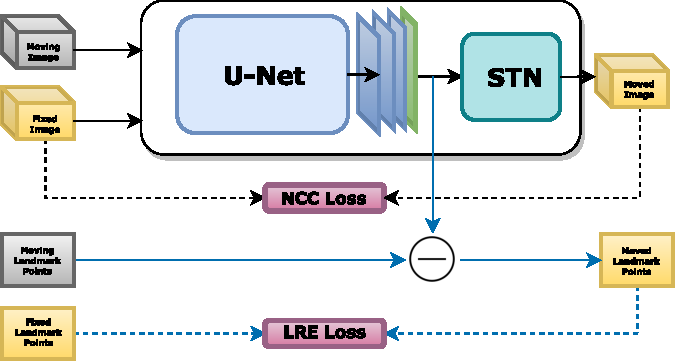
\includegraphics[width=0.6\columnwidth]{resources/chapter4/methods/Method2.pdf}
		\caption{A visual guide to train ``Landmark Guided Voxelmorph" model with landmark points as auxiliary information.}
		\label{fig:block_method2}
	\end{figure}

	\section{``Cascaded Vanilla Voxelmorph": Gaussian pyramid filtering and cascaded training.}
	Image registration is a challenging task because the optimization surface can be complex and lead to suboptimal results if the model gets stuck in such a local optimum. However, literature studies have shown that performing registration in a coarse-to-fine manner can help the model escape such local optima and achieve one of the better global optima. This approach has proven successful in both the pre-deep learning and deep learning eras.
	
	In this method, called ``pyramid registration," pyramidal Gaussian filters are applied and the images are aligned from the lowest to the highest resolution. This method is effective because it ensures that the images are first aligned with the large structures at the lowest resolutions and then progressively aligned with the finer structures as the resolution increases.
	
	Thus, the method consists of processing an image at five different resolutions and aligning the images from coarse to fine, starting with the lowest resolution and gradually increasing the resolution at each stage. In each stage, the transformation learned in the previous stage is cascaded to the current stage. To decrease the resolution of the image, a Gaussian blur with different values for $\sigma$ is applied while the width and height of the image remain constant. This process can be represented mathematically with the equation for Gaussian blur \ref{eqn:GaussBlur}.
	
	Let's say we have an input image with pixel values $I(x, y)$, and we want to apply Gaussian blurring to it using a kernel with size $n \times n$. The resulting image, $G(x, y)$, can be computed as follows:
	
	\begin{equation}\label{eqn:GaussBlur}
		G(x, y) = \frac{1}{Z} \sum_{s=-\frac{n}{2}}^{\frac{n}{2}}\sum_{t=-\frac{n}{2}}^{\frac{n}{2}}I(x+s, y+t) \cdot K(s, t)
	\end{equation}
	
	where $K(s, t)$ is the Gaussian kernel and $Z$ is a normalization factor. The Gaussian kernel is defined as:
	
	\begin{equation}
		K(s, t) = \frac{1}{2\pi \sigma^2} \exp\left(-\frac{s^2+t^2}{2\sigma^2}\right)
	\end{equation}
	
	Here, $\sigma$ is a parameter that determines the amount of blur applied to the image. A larger value of $\sigma$ results in more blur. The size of the kernel, $n$, is usually chosen to be an odd number such as 3, 5, or 7. We start by processing the image at the lowest resolution, where the value of $\sigma$ is set to 4. In subsequent stages, we progressively increase the resolution of the image by decreasing the value of $\sigma$ to 2, 1, 0.5, and finally to 0, which is the original resolution of the image.
	The process is illustrated in the Figure \ref{fig:block_Cascaded Vanilla Voxelmorph}.
	
    \begin{figure}[h!]
		\centering
		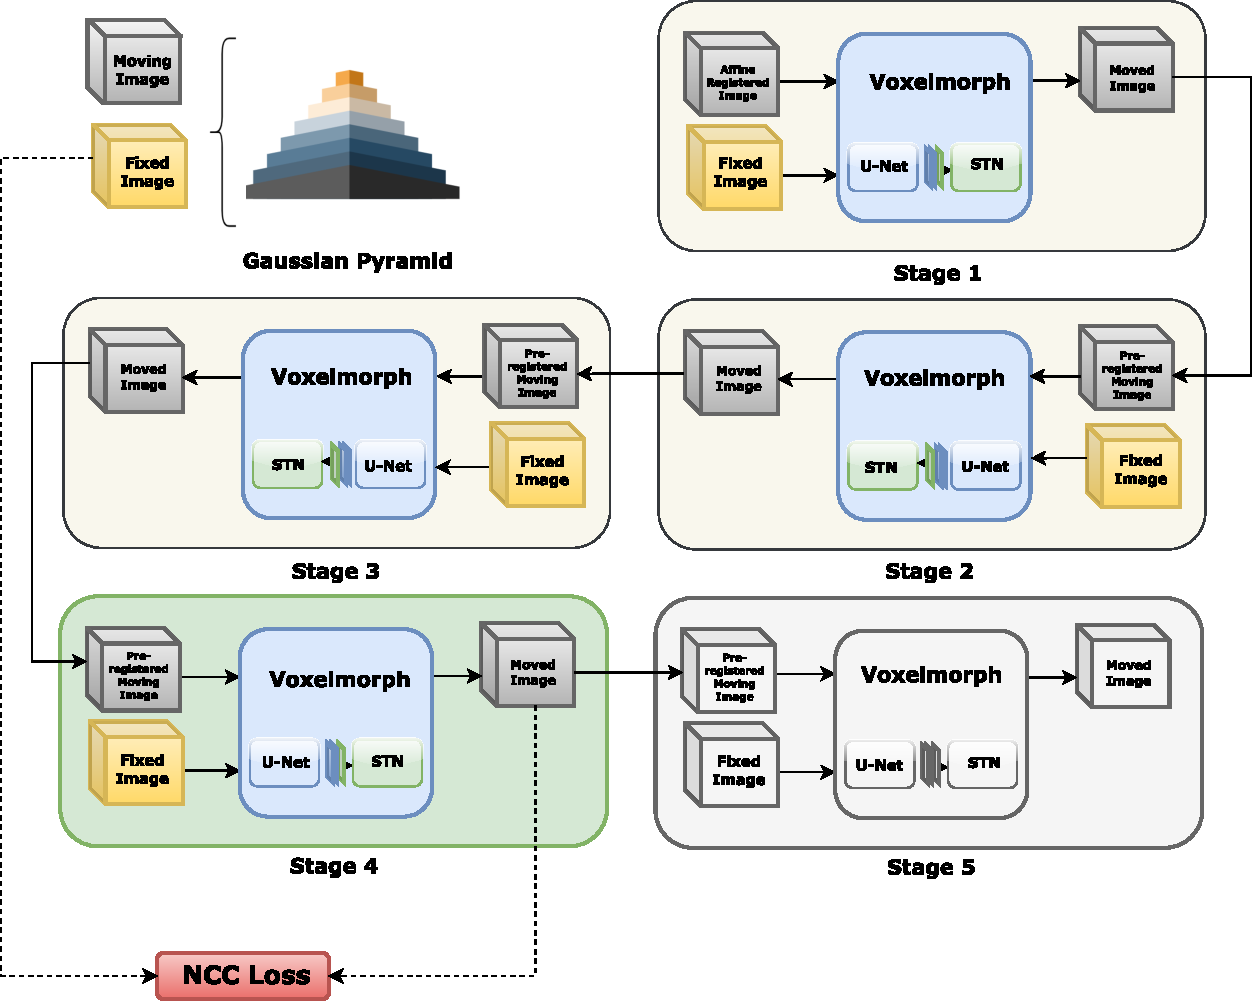
\includegraphics[width=\columnwidth]{resources/chapter4/methods/Method3.pdf}
		\caption{Registration process with ``Cascaded Vanilla Voxelmorph" involves 5 stages, each of which is trained independently. At any given time, only one stage (colored green) is trained, while the other stages (colored white or gray) are either frozen or not in use. The input for the current stage (colored green) is selected from a list of Gaussian filtered images and passes through the previous stages (colored white) to be pre-registered before being used for training. The stages located after the current stage (colored gray) are not utilized during this training process.}
		\label{fig:block_Cascaded Vanilla Voxelmorph}
	\end{figure}

	In this method of image registration, multiple Voxelmorph models are cascaded together without any auxiliary information, using the same model configurations as vanilla Voxelmorph and ``Landmark Guided Voxelmorph". Both the moving and fixed images are preprocessed with Gaussian blur, using appropriate sigma values for each stage.
	
	\subsection{Stages}
	For each stage, the appropriate inputs (fixed image and moving image) are chosen from the Gaussian pyramid. To help explain the process, we will refer to the inputs for each stage as \texttt{input1} through \texttt{input5}, with \texttt{input1} representing the input images for stage 1 (blurred with sigma = 4), \texttt{input2} representing the input images for stage 2 (blurred with sigma = 2), and so on. The final input, \texttt{input5}, consists of the original, unmodified images. We will also refer to the models for each stage as \texttt{model1} through \texttt{model5}. The same optimization function (Normalized Cross-Correlation) is used in all these stage and aims to maximize the similarity between the moved and fixed images.
	
	\begin{equation}
		L = -\frac{1}{N} \sum_{i=1}^N \text{NCC}(Fixed, Moved_i)
	\end{equation}
	
	where:
		$\text{L}$ is the loss function, $N$ is the number of moving images, $\mathbf{Moved}_i$ is the $i$th moved image, $\mathbf{Fixed}$ is the fixed image, and $NCC(\mathbf{Fixed}, \mathbf{Moved}_i)$ is the Normalized Cross-Correlation between the $i$th moved image and the fixed image.
	
	\subsubsection{Stage 1}
	In stage 1, the model is trained using input images that has been pre-processed with Gaussian blurring using sigma = 4. The predicted deformation field from this model is used to transform the input image, creating a version called the ``moved image." This moved image is then compared to the fixed image, which has also been pre-processed with Gaussian blurring using sigma = 4. All other later stages are not used and is grayed out.
	
	\subsubsection{Stage 2}
	In stage 2, the model is trained using input images that have been pre-processed with a Gaussian blur of sigma = 2. After completing the training for stage 1, the trained model parameters are frozen (white) and used for coarse alignment of \texttt{input2} images. These coarsely aligned \texttt{input2} images are then used to train stage 2 to predict a deformation field, which is applied to the input moving image using a spatial transformer network (STN) to produce a transformed moving image called the ``moved image". The moved image is compared to the fixed image, which has been pre-processed with a Gaussian blur of sigma = 2, to compute the similarity value. The later stages are grayed out.
	
	\subsubsection{Stage 3, 4 and 5}
	The aforementioned steps are repeated iteratively for all subsequent stages, using the previously trained and frozen models to incorporate the learned transformation and coarsely align the images for the current training stage. This process follows a coarse-to-fine approach, meaning that the transformation is initially learned at a coarser resolution and then successively refined at finer resolutions.
	
	\section{``Cascaded Landmark Guided Voxelmorph": Gaussian pyramid filtering with novel landmark information and cascaded training.}
	In ``Landmark Guided Voxelmorph", the use of landmark information was found to improve performance. However, incorporating this information in ``Cascaded Landmark Guided Voxelmorph" is not as straightforward because the input for each stage consists of different pre-aligned images, which means that landmarks annotated in one stage cannot be used in later stages as they are moved to different positions by the process of pre-alignment. Manually re-annotating the landmarks for each stage is impractical, especially when there are many stages or a large number of images. To solve this problem, we have developed a method that allows us to incorporate landmark information at all stages without the need for manual re-annotation. Our approach is based on the fact that the input images are the same for each phase, except for the different levels of applied Gaussian blur. This means that the initial annotations made on any of these images can be used in later stages if we can transfer the landmarks to their new positions using the predicted deformation field, similar to the pre-alignment process for images.
	
	Again, this is a novel method introduced as part of this work. These shifted landmarks, called ``pseudo-annotated" landmarks, may not be as accurate as manually annotated landmarks, but they were accurate enough to work with the blurred images in the earlier stages where the structures were not clear and did not require precise manual annotation.
	
	The equation~\ref{eq:ldm_prop} states that the new landmark position is determined by subtracting the deformation field at that position from the old landmark position.
	
	\begin{equation}\label{eq:ldm_prop}
		l_n^{new} = l_n^{old} - d_n
	\end{equation}
	
	where:
	
	$l_n^{new}$ is the new position of the landmark in image $n$. $l_n^{old}$ is the old position of the landmark in image $n$. $d_n$ is the deformation field for image $n$ at the position of the landmark.
	
	``Cascaded Landmark Guided Voxelmorph" combines aspects of ``Landmark Guided Voxelmorph" and ``Cascaded Vanilla Voxelmorph" in an attempt to leverage the strengths of both the approaches. As with ``Cascaded Vanilla Voxelmorph", an image is processed at five different resolutions and aligned coarse to fine, starting with the lowest resolution and increasing it incrementally at each stage. The transformation learned in the previous stage is cascaded to the current stage. To reduce the resolution of the image, a Gaussian blur with different sigma values is applied while keeping the width and height of the image constant. This process is represented mathematically with the equation \ref{eqn:GaussBlur}. And as in ``Landmark Guided Voxelmorph", we use the auxiliary information in the form of landmarks to train the neural network in the right direction.
	
	\subsection{Stages}
	For each stage, the corresponding inputs (fixed image and moving image) are selected from the Gaussian pyramid. To explain the process, the inputs for each stage are labeled \texttt{input1} through \texttt{input5}, where \texttt{input1} represents the input images for stage 1 (blurred with sigma = 4), \texttt{input2} represents the input images for stage 2 (blurred with sigma = 2), and so on. The final input, \texttt{input5}, consists of the original, unmodified images. We also refer to the models for each stage as \texttt{model1} through \texttt{model5}. The same optimization function (Normalized Cross-Correlation) is used in all these stages and it aims to maximize the similarity between the moving and the fixed images. In addition, the model is also evaluated based on the landmark registration error to guide the learning process.
	
	Therefore, the optimization function attempted to minimize was:
	\begin{equation}\label{eq:aux_loss_combined}
		L_\text{combined} = L_\text{main} + L_\text{aux}
	\end{equation}
	
	Let us call the main loss as $L_\text{main}$ and the landmark registration error as $L_\text{aux}$.
	
	\textbf{Main loss:}
	\begin{equation}\label{eq:aux_loss_main}
		L_\text{main} = -\frac{1}{N} \sum_{i=1}^N \text{NCC}(Fixed, Moved_i)
	\end{equation}
	
	\textbf{Landmark registration error:}
	\begin{equation}\label{eq:aux_loss_aux}
		L_\text{aux} = \frac{1}{NL} \sum_{n=1}^N \sum_{l=1}^L \sqrt{(p_l - q_{n,l})^2}
	\end{equation}
	
	In the equation~\ref{eq:aux_loss_main}, $N$ is the number of moving images, $\mathbf{Moved}_i$ is the $i$th moved image, $\mathbf{Fixed}$ is the fixed image, and $NCC(\mathbf{Fixed}, \mathbf{Moved}_i)$ is the Normalized Cross-Correlation between the $i$th moved image and the fixed image. The loss function is the negative average of the Normalized Cross-Correlation between the fixed image and each of the moving images.
	
	In this Equation~\ref{eq:aux_loss_aux}, $N$ is the number of moving images, $L$ is the number of landmarks, $p\_l$ is the coordinates of the l-th landmark in the fixed image, and $q\_{n,l}$ is the coordinates of the l-th landmark in the n-th moving image. The auxiliary loss is the average of the euclidean distance between the landmarks in the fixed image and the landmarks in each of the moving images.
	
    The whole process is described in the Figure~\ref{fig:block_method4} and the following pseudo code \ref{lst:ldm_propogation} demonstrates how landmarks are propagated from stage 1 to stage 's' by utilizing the deformation model at each stage.
    
    \begin{lstlisting}[language=Python, label=lst:ldm_propogation, caption=Pseudo code to show how the landmarks are propogated from stage to stage.]
    	# N: The number of landmark lists.
    	# M: The number of landmark points in each landmark list.
    	# S: The number of stages.
    	for n in range(N):
    	# n: The index of the current landmark list.
    	for m in range(M):
    	# m: The index of the current landmark point.
    	for s in range(S):
    	# s: The index of the current stage.
    	# deformation_field: The deformation field for the current stage.
    	deformation_field = find_deformation_field(s)
    	# old_landmark_point: The old landmark point for the current landmark point
    	# and stage.
    	# new_landmark_point: The new landmark point for the current landmark point
    	# and stage, which is calculated by subtracting the deformation field from
    	# the old landmark point.
    	new_landmark_point = old_landmark_point - deformation_field
    	# Update the landmark point with the new value.
    	update_landmark_point(new_landmark_point)
    \end{lstlisting}

	\subsubsection{Stage 1}
	In stage 1, the model is trained using input images preprocessed with a Gaussian blur of sigma = 4. The deformation field predicted by this model is used to transform the moving image and create a version called the ``moved image". This moved image is then compared to the fixed image, which has also been preprocessed with Gaussian blur of sigma = 4. All the later stages are not used and are grayed out.

	\subsubsection{Stage 2}
	In stage 2 of this process, the model is trained on input images that have been blurred using a Gaussian blur with a sigma value of 2. The trained model from stage 1 is then frozen and used to coarsely align the \texttt{input2} images. These aligned images are used to train stage 2 to predict a deformation field, which is applied to the input moving image using a spatial transformer network (STN) to create a transformed image called the ``moved image". The moved image is compared to the fixed image, which has also been blurred using a Gaussian blur with a sigma value of 2, to calculate a similarity value. Stage 2 uses ``pseudo-annotated" landmarks obtained by propagating manually annotated landmarks from the previous stage using the deformation field predicted by \texttt{model1}.
	
	\begin{equation}\label{eq:pseudoldm}
		landmark_{stage2,m,n} = landmark_{stage1,m,n} - deformation\_field_{stage1,m,n}
	\end{equation}
	
	Here, 
	\begin{itemize}
		\item ``$landmark_{stage2,m,n}$" is the landmark point for stage 2 at pixel m for image n.
		\item ``$landmark_{stage1,m,n}$" is the landmark point for stage 1 at pixel m for image n.
		\item ``$deformation\_field_{stage1,m,n}$" is the deformation field from stage 1 at pixel m for image n.    
	\end{itemize}
	
	This Equation~\ref{eq:pseudoldm} is valid for all values of m such that m is a landmark point for an image in stage 1, and for all values of n such that n belongs to N, where N is the number of images in stage 2.

	\begin{figure}[p!]
		\centering
		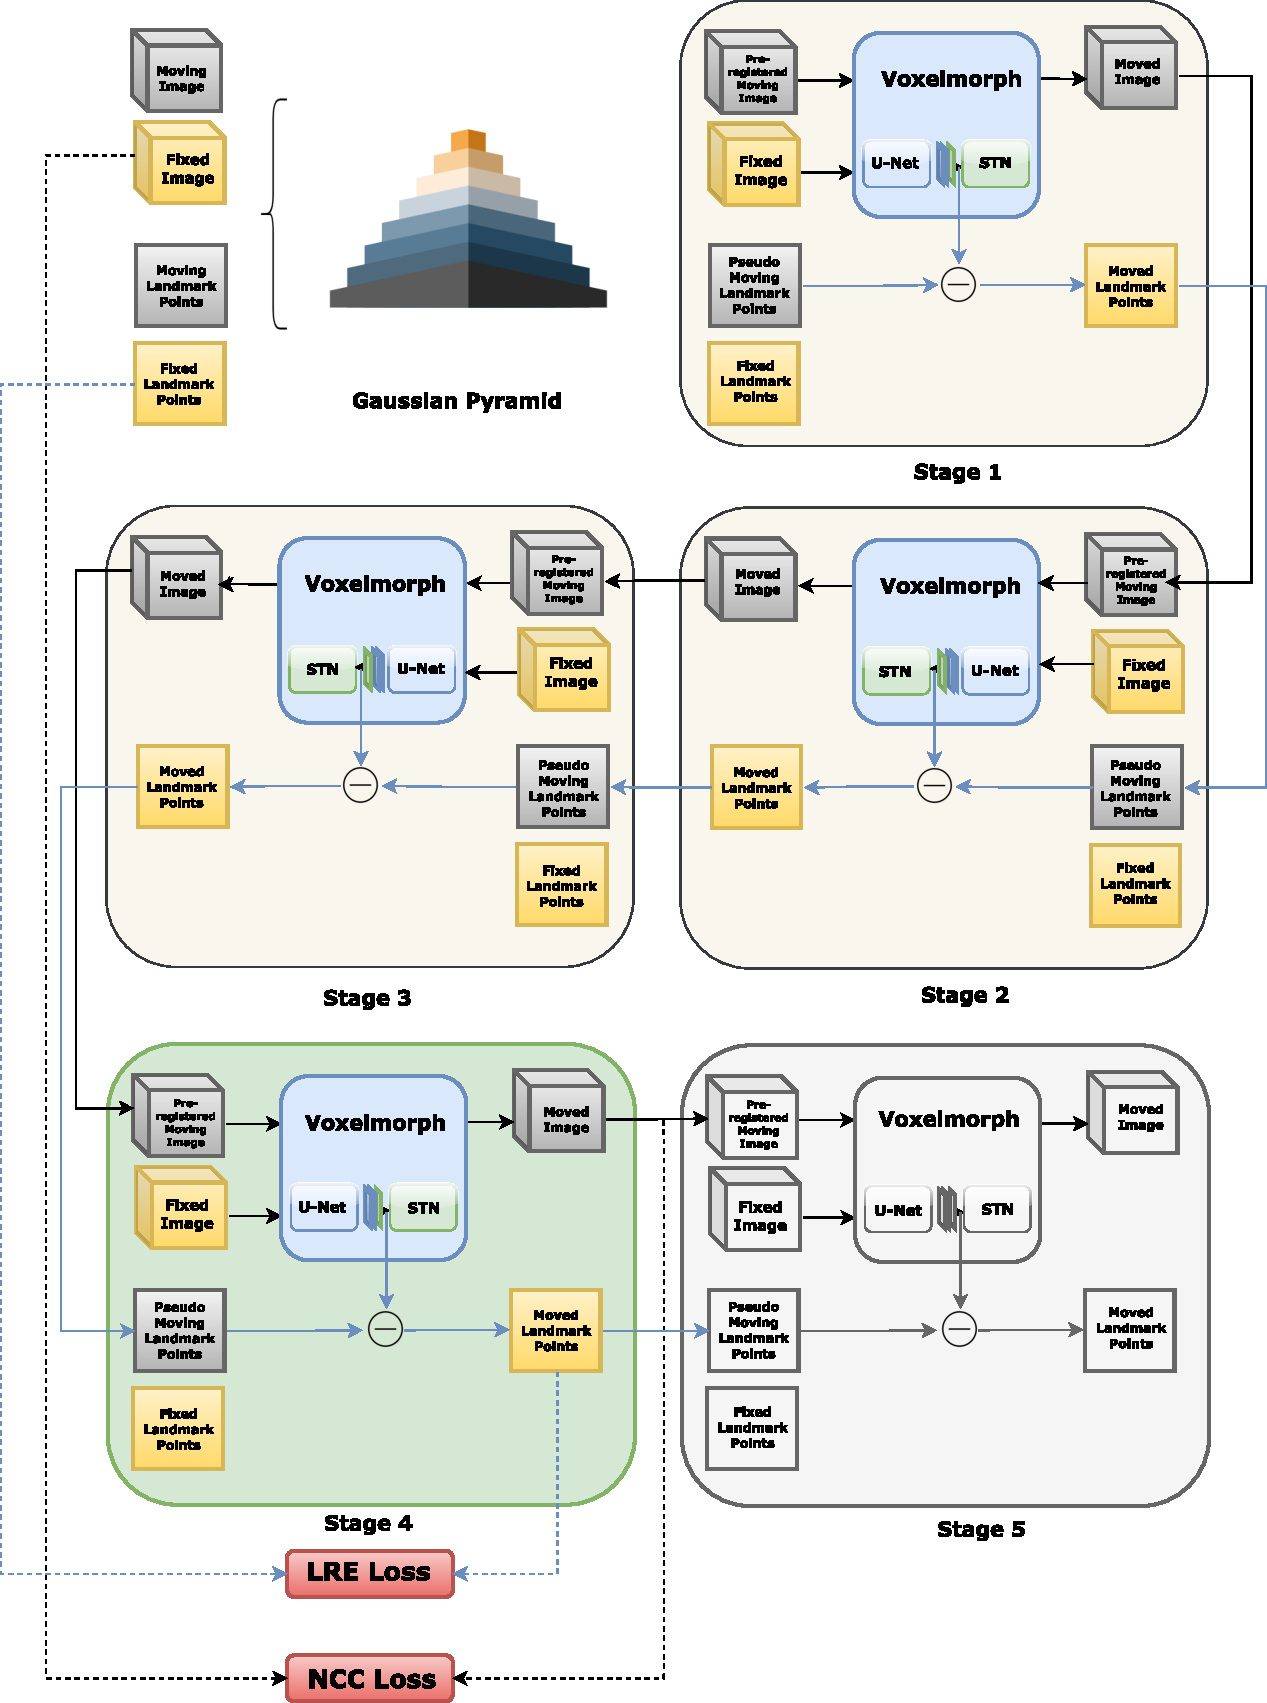
\includegraphics[width=\columnwidth]{resources/chapter4/methods/Method4.pdf}
		\caption{Registration process with ``Cascaded Landmark Guided Voxelmorph" consists of 5 stages, each of which is trained separately. Only one stage (indicated by the color green) is being trained at a given time, while the other stages (colored white or gray) are either inactive or not being used. The input for the current stage (colored green) is selected from a list of Gaussian filtered images and passes through the previous stages (colored white) to be pre-registered before being used for training. The stages that come after the current stage (colored gray) are not used during this training process. In addition to the images, the landmark points are also used to calculate the Landmark Registration Error (LRE) at each stage during training.}
		\label{fig:block_method4}
	\end{figure}
	
	\subsubsection{Stage 3 and 4}
	The above steps are iteratively repeated for all subsequent stages, using the previously trained and frozen models to integrate the learned transformation and coarsely align the images for the current training stage. This process follows a coarse-to-fine approach, i.e., the transformation is first learned at a coarser resolution and then successively refined at finer resolutions.
	
	\subsubsection{Stage 5: The last stage}
	The original approach to aligning the images in the final stage of the process was to transfer the previously identified landmarks via software. However, it was eventually decided to manually label the landmarks again to improve accuracy. The reason for this is that the images used in this phase are the original untouched images and the use of landmarks generated using the previous, already aligned images may not be accurate enough. By manually labeling the landmarks, the final registration can be more accurate.
	
	\chapter{Results}\label{chapter:results}
	This chapter presents the results of the research study conducted to investigate whether the use of Deep Learning Neural Networks would result in rapid and robust image registration of the larval brain of Drosophila. The results are presented clearly and objectively, and all statistical analyses that were performed are included to support the data. We will divide this chapter into two sections ~\nameref{sec:Qualitative} and ~\nameref{sec:Quantitative}. The \nameref{sec:Quantitative} section provides a detailed analysis of the data collected by performing registration using the ``Cascaded Vanilla Voxelmorph" and ``Cascaded Landmark Guided Voxelmorph" methods, and presents the results in a logical and coherent manner.
	
	\section{Qualitative Analysis} \label{sec:Qualitative}
	In the following subsections, we will provide a qualitative analysis of the results obtained using the methods explained in the chapter~\nameref{chap:methods}. Qualitative evaluation is the use of subjective observations and interpretations to assess the performance of our methods. To do this, we overlay the registered image with the fixed image and look for regions where there is no overlap. The registered images and the fixed image used for the overlay are the projection of the maximum intensity of the respective 3D volumes. This is sufficient to visualize the alignment in xy direction.
	
	\subsection{Results for vanilla Voxelmorph}
	The model with the configurations mentioned in the previous chapter was trained with the \texttt{Janelia dataset} and tested on the \texttt{Larvalign dataset}. It was found that this model performed poorly on images that contained large deformations as shown in the Figure~\ref{fig:method1_fail}. However, on images with small deformations, as shown in the Figure~\ref{fig:method1_pas}, the model performed good. This suggested that the vanilla Voxelmorph model may be less effective at registering images with large deformations.
	
	\begin{figure}[h]
		\centering
		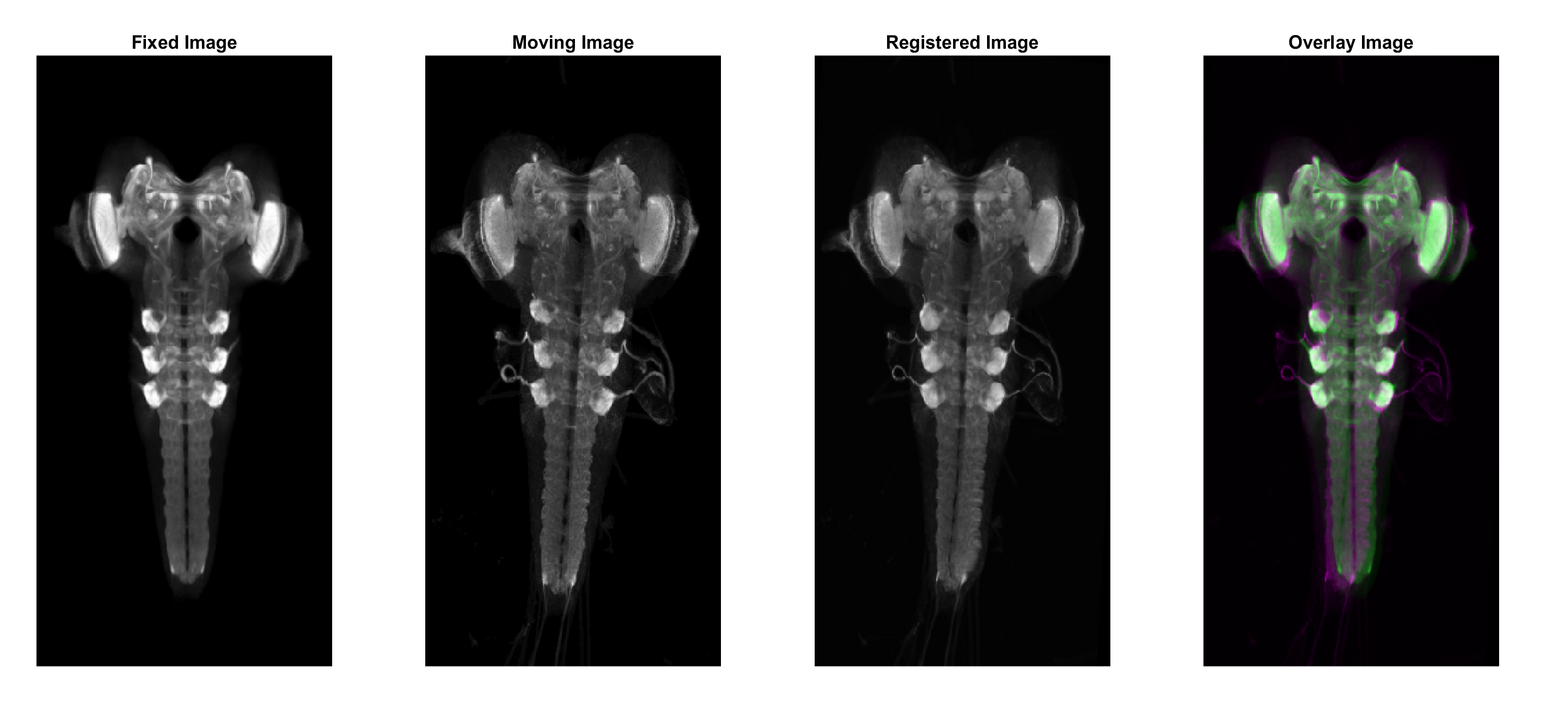
\includegraphics[width=0.8\columnwidth]{resources/chapter4/np_60H12_14E09_MB049B_020113B_scaled.tif.png}
		\caption{An example moving sample image with larger deformation where the vanilla Voxelmorph did not produce a successful result.}
		\label{fig:method1_fail}
	\end{figure}

	\begin{figure}[h]
		\centering
		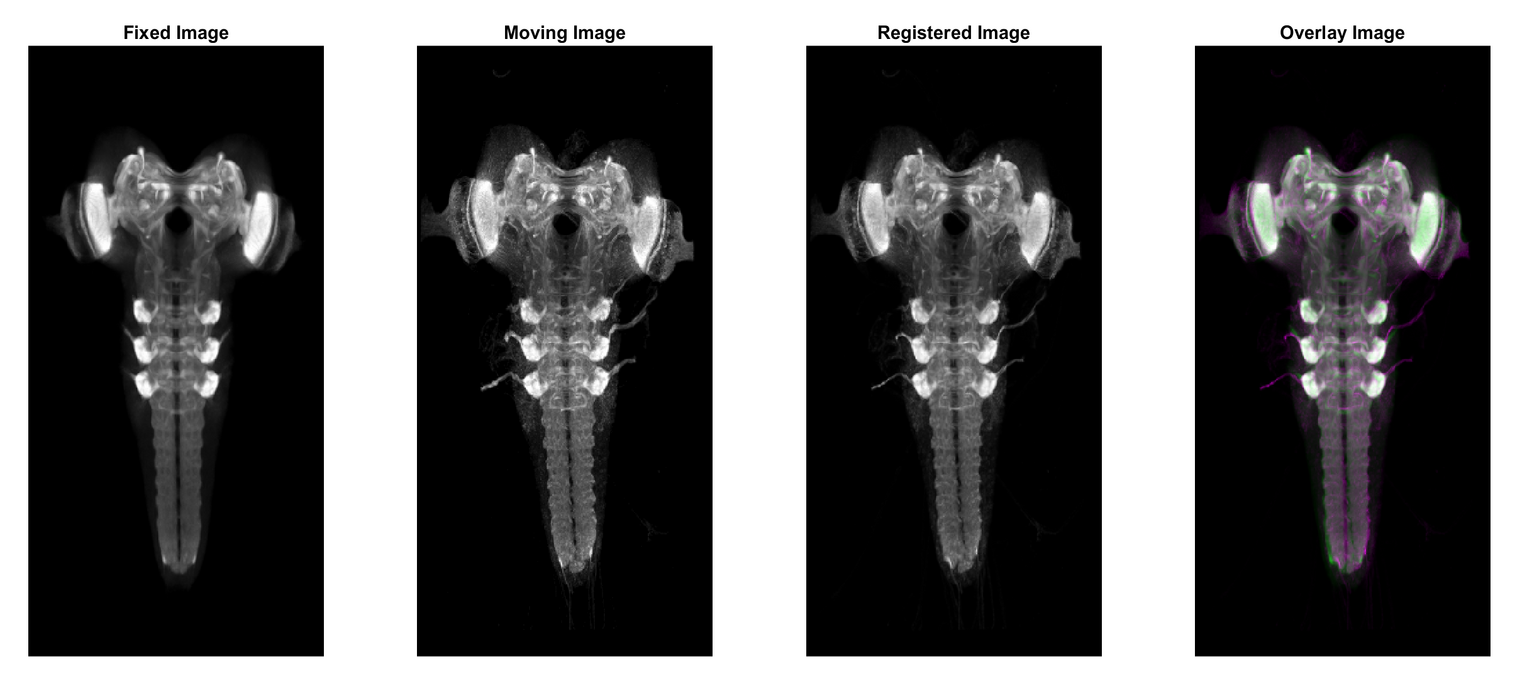
\includegraphics[width=0.8\columnwidth]{resources/chapter4/np_brain7_scaled.tif.png}
		\caption{An example moving sample image with smaller deformation where the vanilla Voxelmorph produced a successful result.}
		\label{fig:method1_pas}
	\end{figure}

	The first image is the fixed image against which the registration is being performed. The second image is the moving image that is being registered. The third image is the result of the registration process, and the fourth image is an overlay of the registered image and the fixed image.
	
	The moving image in Figure~\ref{fig:method1_fail} has large deformation at the lower end of the ventral nerve cord (VNC), and the registration process is not successful as evident (magenta region at the lower tip of VNC) in the corresponding overlay image. In contrast, the Voxelmorph method produces good results in the Figure~\ref{fig:method1_pas}. The good results produced by the Voxelmorph method in this case can be attributed to the absence of significant deformation in the moving image and the model's ability to handle smaller deformations.

	
	\subsubsection{Motivation for ``Landmark Guided Voxelmorph"} \label{subsec:motivation_for_method2}
	The model clearly had difficulty dealing with large deformations, especially in the lower part of the ventral nerve cord of the brain. To improve the performance of the model in these cases, we can provide it with additional manually labeled information for both the moving and fixed images. This can help the model to achieve better alignment, especially for large deformations. The proof of this concept will be tested and evaluated in the next method.
	
	The addition of additional manually labeled information in the form of landmarks for both the moving images and the fixed image is referred to as ``Landmark Guided Voxelmorph".
	
	\subsection{Results for ``Landmark Guided Voxelmorph"}
	Using the same model configurations as in vanilla Voxelmorph, landmark points were included as auxiliary information in the training. The model was trained using the \texttt{Janelia dataset} and tested using the \texttt{Larvalign dataset}. It was found that the registration accuracy was improved in the regions with landmarks.
	
	\begin{figure}[h!]
		\centering
		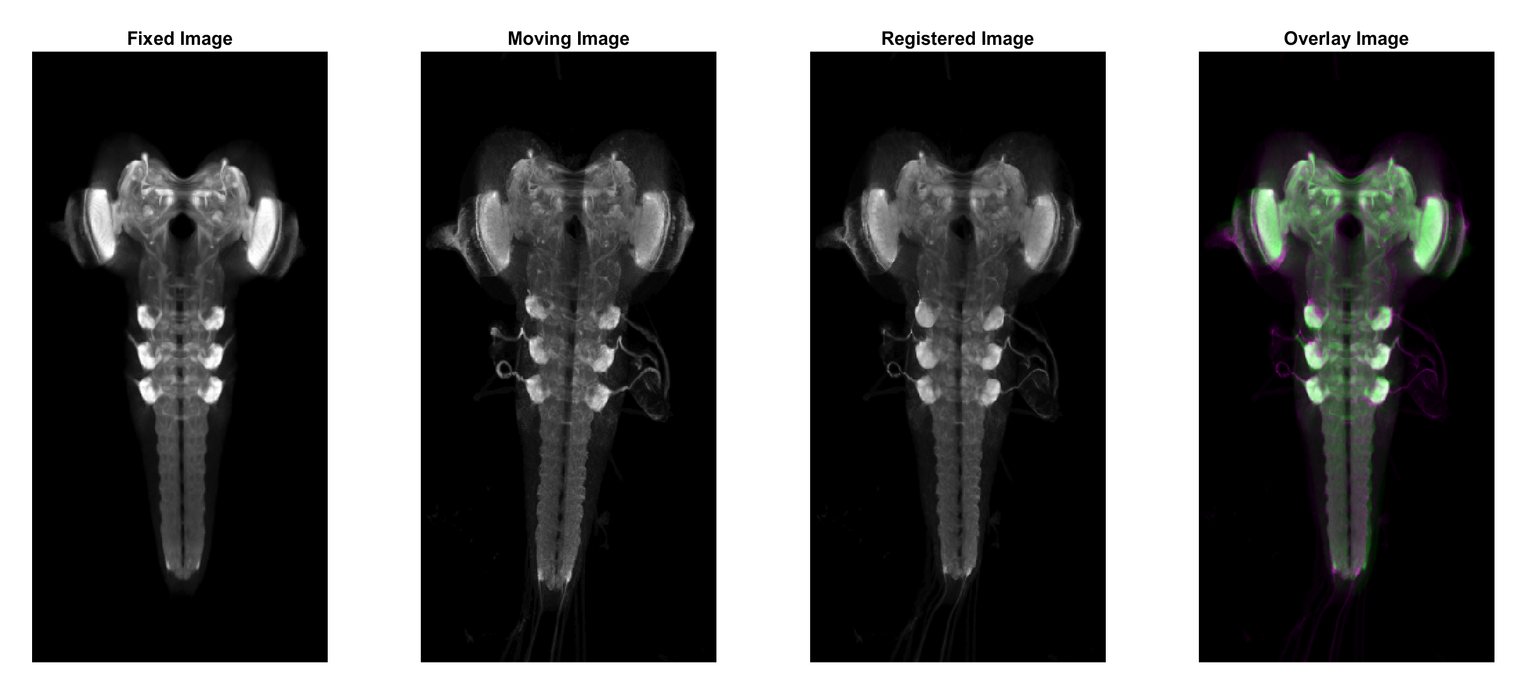
\includegraphics[width=0.9\columnwidth]{resources/chapter4/method2/np_60H12_14E09_MB049B_020113B_scaled.tif.png}
		\caption{An example of a moving sample image with larger deformation where the ``Landmark Guided Voxelmorph", unlike the Vanilla Voxelmorph, can lead to a successful result with large deformations.}
		\label{fig:method2_fail}
	\end{figure}
	
	Figures \ref{fig:method1_fail} and \ref{fig:method2_fail} can help us understand the improvement brought by the ``Landmark Guided Voxelmorph" compared to vanilla Voxelmorph. As can be seen in Figure~\ref{fig:method1_fail}, vanilla Voxelmorph failed to achieve satisfactory registration at the bottom of the VNC. However, in Figure~\ref{fig:method2_fail}, it can be seen that adding landmarks at the VNC tip helped ``Landmark Guided Voxelmorph" to achieve better registration performance. The results in both figures show the effectiveness of using landmark information to improve registration accuracy. For the moving images with small deformations as in Figure~\ref{fig:method1_pas}, the model continued to provide accurate registration results as expected. This can be verified in Figure~\ref{fig:method2_pas}.
	
	\begin{figure}[h!]
		\centering
		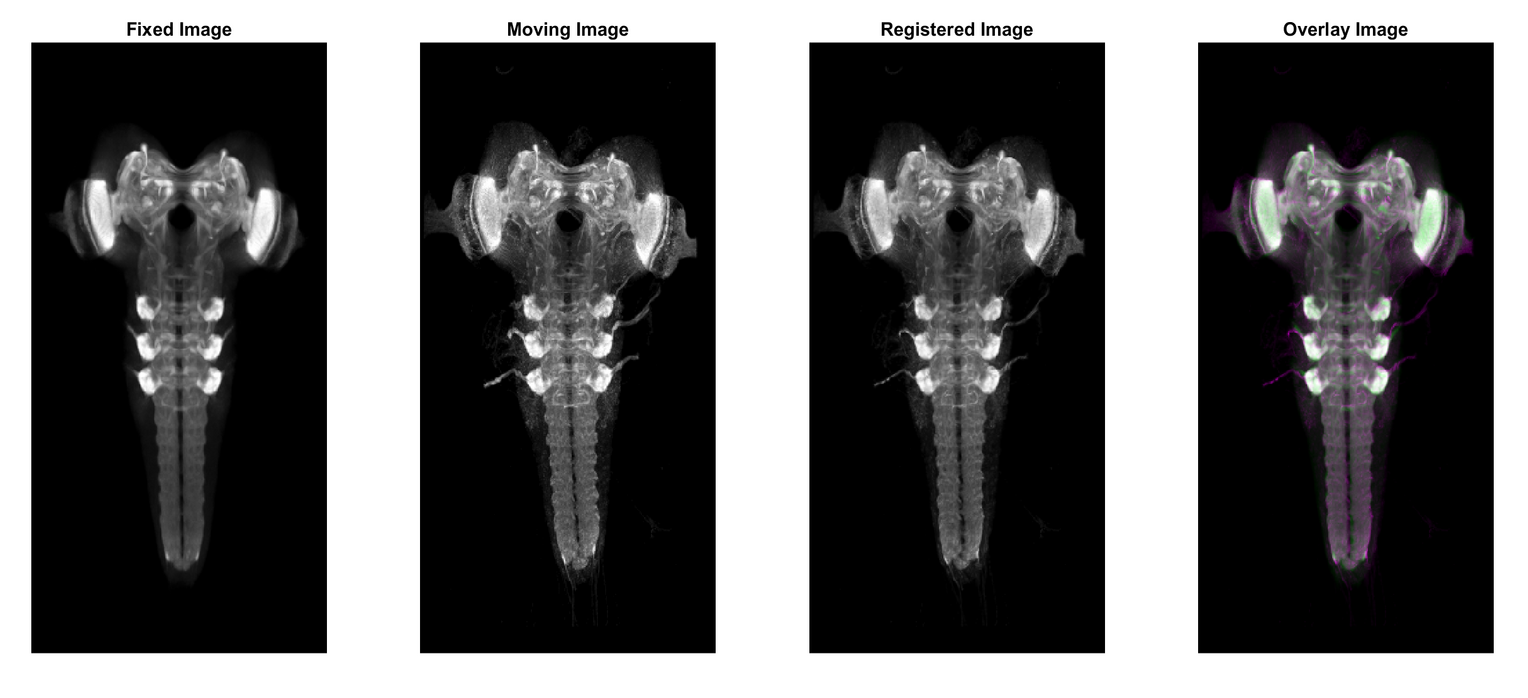
\includegraphics[width=0.9\columnwidth]{resources/chapter4/method2/np_brain7_scaled.tif.png}
		\caption{An example of a moving sample image with smaller deformation where the ``Landmark Guided Voxelmorph" could achieve a successful result like vanilla Voxelmorph.}
		\label{fig:method2_pas}
	\end{figure}
	
	\subsubsection{Motivation for ``Cascaded Vanilla Voxelmorph"}
	The inclusion of landmarks improved registration accuracy, but in some cases, for moving images with significant deformations, this model resulted in artifacts. An example of this can be seen in the following figure Figure~\ref{fig:method2_artifact}. The two images focused on the inferior tip of the ventral nerve cord (VNC) show the moving image before and after registration. As can be seen, the structures in this area appear to have been erased after registration. 
	
	The artifact is commonly observed in moving images with large deformations and may be due to the inherent limitations of the model in handling such large deformations. By adding additional information, an attempt is made to force the model to achieve near-perfect registration, even though it is not yet capable of doing so. This new force in play can cause the network to compromise on qualitative features while still achieving good error values. To fix this problem, the model must be better able to handle large deformations, since the auxiliary information must act as a guide, and if the model is inherently incapable of handling large deformations, the loss due to the auxiliary information begins to play the main role.
	
	\begin{figure}[h!]
		\centering
		\includegraphics[width=0.9\columnwidth]{resources/chapter4/method2/np_52B07_52H01_MB262B_021713B_scaled.png}
		\caption{An example of a moving sample image with large deformations at the inferior tip of the ventral nerve cord (VNC) where the ``Landmark Guided Voxelmorph" produced an artifact in the registered output.}
		\label{fig:method2_artifact}
	\end{figure}
	
	\subsection{Results for ``Cascaded Vanilla Voxelmorph"}
	The cascade of models is trained on the \texttt{Janelia dataset} with the same setup and model configurations as vanilla Voxelmorph and ``Landmark Guided Voxelmorph" and tested on the \texttt{Larvalign dataset}. It was found that the registration of the same moving sample image that produced artifacts with ``Landmark Guided Voxelmorph" now has no such artifacts. This can be seen in Figure~\ref{fig:Cascaded Vanilla Voxelmorph_artifact} and compared to the output in Figure~\ref{fig:method2_artifact}.
	
	\begin{figure}[h!]
		\centering
		\includegraphics[width=0.9\columnwidth]{resources/chapter4/Method3/compare/np_52B07_52H01_MB262B_021713B_scaled.png}
		\caption{An example of a moving sample image with large deformations at the inferior tip of the ventral nerve cord (VNC) where the ``Cascaded Vanilla Voxelmorph" did not produce artifacts in the registered output.}
		\label{fig:Cascaded Vanilla Voxelmorph_artifact}
	\end{figure}
	
	Furthermore, unlike vanilla Voxelmorph, ``Cascaded Vanilla Voxelmorph" provides good registration results for moving images with large and small deformations. This can be seen in the figures~\ref{fig:Cascaded Vanilla Voxelmorph_pas} and \ref{fig:Cascaded Vanilla Voxelmorph_fail}.
	
	\begin{figure}[h!]
		\centering
		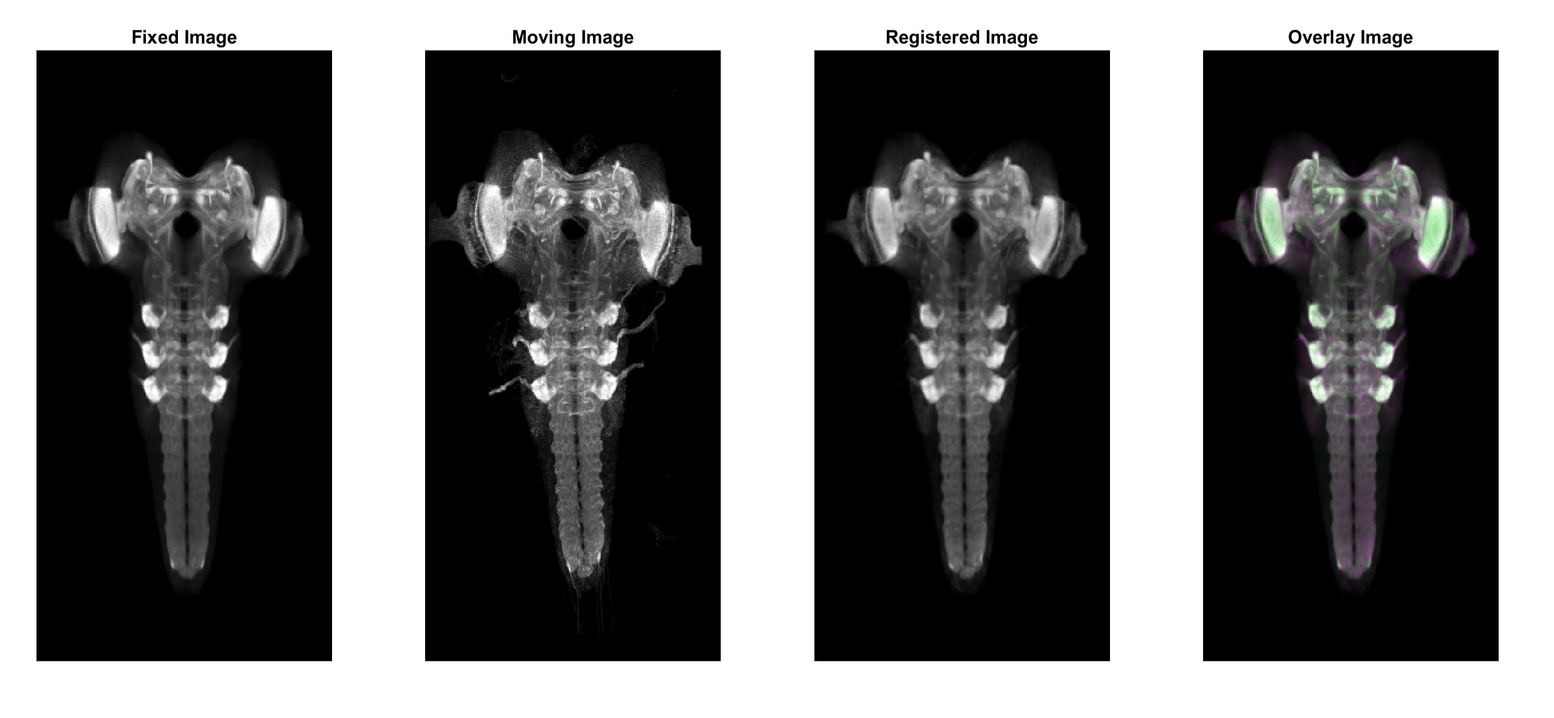
\includegraphics[width=0.9\columnwidth]{resources/chapter4/Method3/compare/np_brain7_scaled.tif.png}
		\caption{An example of a moving sample image with smaller deformation, where the ``Cascaded Vanilla Voxelmorph" could still provide a successful result like vanilla Voxelmorph and ``Landmark Guided Voxelmorph".}
		\label{fig:Cascaded Vanilla Voxelmorph_pas}
	\end{figure}
	
	\begin{figure}[h!]
		\centering
		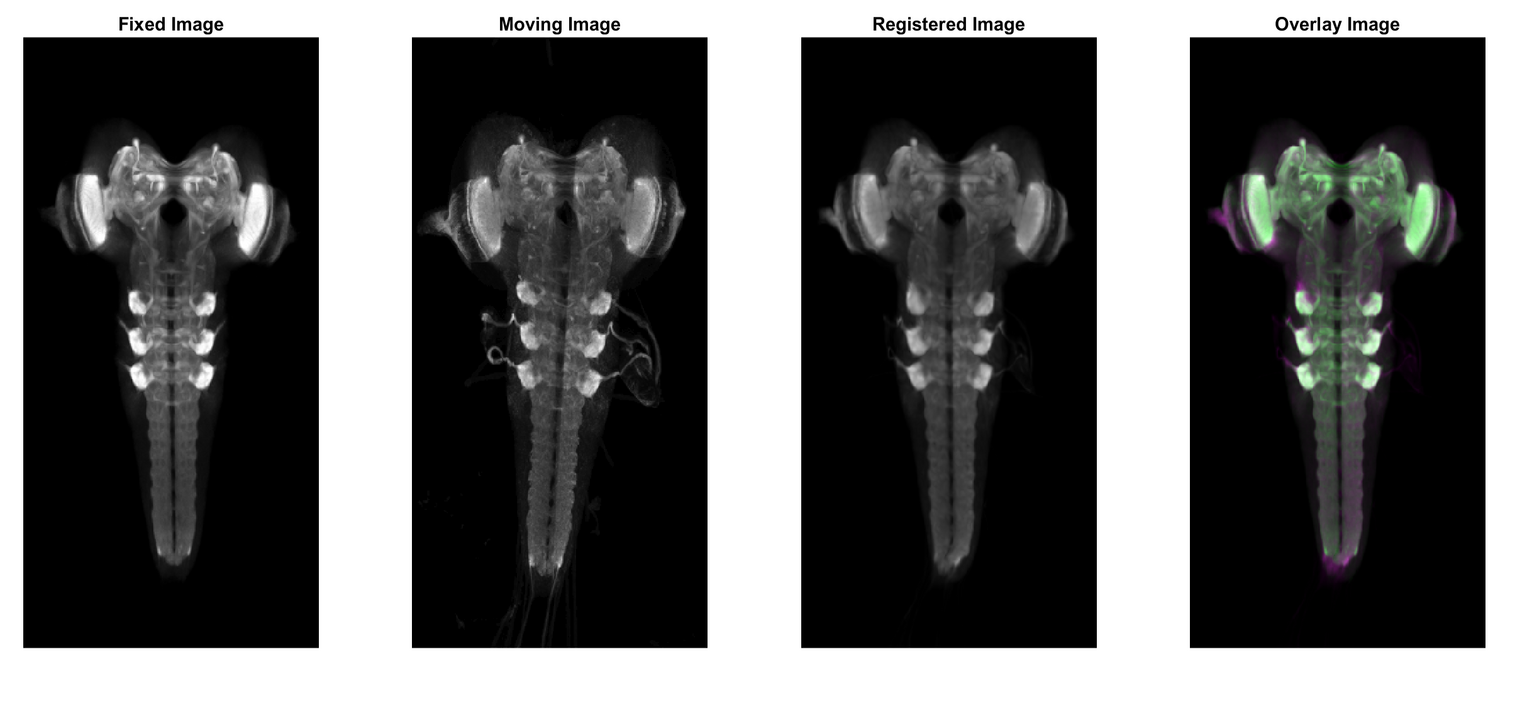
\includegraphics[width=0.9\columnwidth]{resources/chapter4/Method3/compare/np_60H12_14E09_MB049B_020113B_scaled.tif.png}
		\caption{An example of a moving sample image with larger deformation, where the ``Cascaded Vanilla Voxelmorph" type of deformable registration could lead to a successful result at large deformations, unlike vanilla Voxelmorph.}
		\label{fig:Cascaded Vanilla Voxelmorph_fail}
	\end{figure}
	
	\begin{figure}[h!]
		\centering
		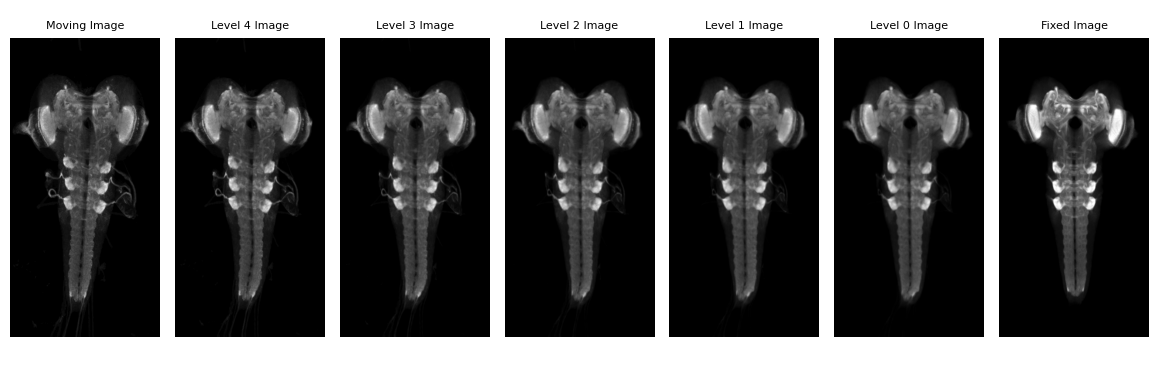
\includegraphics[width=0.9\columnwidth]{resources/chapter4/Method3/np_60H12_14E09_MB049B_020113B_scaled.png}
		\caption{The figure presents the progression of output registration through multiple stages of the ``Cascaded Vanilla Voxelmorph" method. The method is applied in a coarse-to-fine fashion, with each stage utilizing a different resolution level for training. The lowest resolution level is represented by level 4, and the highest resolution level is represented by level 0. The plots demonstrate a clear improvement in registration accuracy as the resolution level increases from level 4 to level 0.}
		\label{fig:Cascaded Vanilla Voxelmorph_cascade}
	\end{figure}
	
	Figure~\ref{fig:Cascaded Vanilla Voxelmorph_cascade} shows the output of the registered moving image as it passes through the stages of the cascade. The corrections are applied from coarse to fine, with the transformation becoming more precise at higher and higher resolutions as the sample passes through them.
	
	\subsubsection{Motivation for ``Cascaded Landmark Guided Voxelmorph"}
	The results show that this method could handle large deformations better than the vanilla Voxelmorph model or ``Landmark Guided Voxelmorph" without artifacts. Although the results were satisfactory, the inclusion of landmark information during training could improve the registration results, as seen in ``Landmark Guided Voxelmorph". In the next method, we will investigate this.
	
	\subsection{Results for ``Cascaded Landmark Guided Voxelmorph"}
	Figure~\ref{fig:method4_combine} consists of 3 moving image samples in 3 rows. Each column represents the output of the corresponding moving image over different stages of the cascaded network. This figure is representative of the output of ``Cascaded Landmark Guided Voxelmorph". Similarly, the Figure~\ref{fig:method3_combine} consists of the same 3 moving image samples in 3 rows each. Each column in turn represents the output of the corresponding moving image in the different stages of the cascaded network. This figure is representative of the output of ``Cascaded Vanilla Voxelmorph".
	
	Comparing Figure~\ref{fig:method4_combine} and Figure~\ref{fig:method3_combine}, it is clear that the addition of landmarks at the lower end of the ventral nerve cord results in better registration accuracy for ``Cascaded Landmark Guided Voxelmorph" than for ``Cascaded Vanilla Voxelmorph".
	
	\begin{figure}[h!]
		\centering
		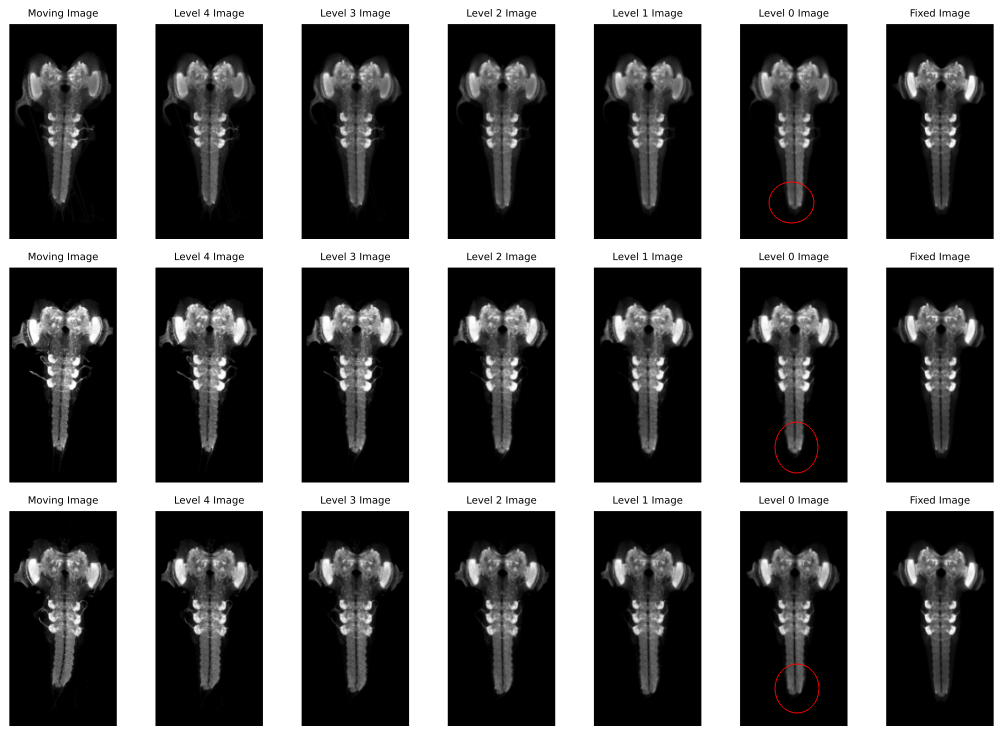
\includegraphics[width=\columnwidth]{resources/chapter4/method4/ldm/registered_images.png}
		\caption{Coarse-to-fine registration with ``Cascaded Landmark Guided Voxelmorph" method.}
		\label{fig:method4_combine}
	\end{figure}
	
	\begin{figure}[h!]
		\centering
		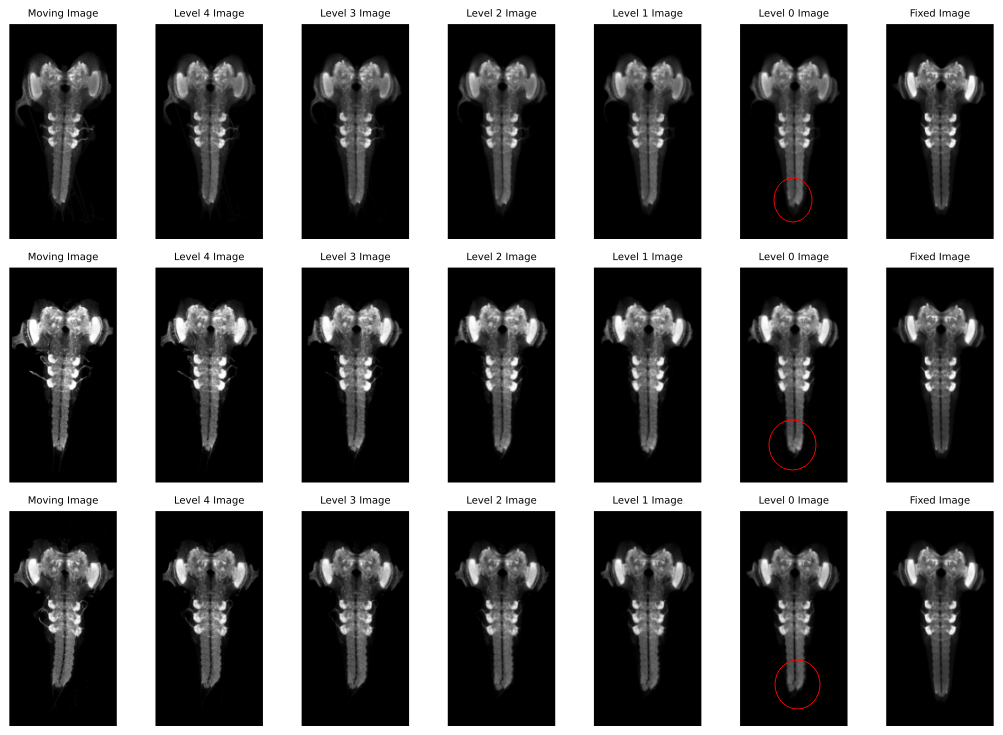
\includegraphics[width=\columnwidth]{resources/chapter4/method4/vanilla/registered_images.png}
		\caption{Coarse-to-fine registration with ``Cascaded Vanilla Voxelmorph" method.}
		\label{fig:method3_combine}
	\end{figure}

	\section{Quantitative analysis} \label{sec:Quantitative}
	So far, we have done qualitative analysis by visually inspecting the registered images and now we know that among all four methods, ``Cascaded Vanilla Voxelmorph" and ``Cascaded Landmark Guided Voxelmorph" are the two most promising methods. So in this section, we will perform the quantitative analysis of these two methods compared to \emph{larvalign}. We perform the analysis to systematically and objectively analyze and interpret the result and compare it with the numbers for the \textit{larvalign} method, which will serve as the baseline. We will use the metrics presented in the \textit{larvalign} \cite{larvalign}, which are also formally defined in the \nameref{sec:quality} section of the chapter~\nameref{chap:imp_and_data}.
	
	Four scores are recorded in the evaluation - three of them measure the Mattes Mutual Information between the registered and the fixed images globally and locally, and another score that measures the landmark registration error (LRE) between the registered and the fixed images. 
	
	The \texttt{Larvalign dataset} is divided into ``good", ``medium", and ``random" sets depending on the quality of the scans and we will use this to report the performance of our methods as a function of the quality of the scans.	

	\begin{comment}
	The table~\ref{table:quality_larvalign_good} records the score for the good quality images of the \texttt{\texttt{Larvalign dataset}}, the table~\ref{table:quality_larvalign_medium} the score for the medium quality images of the \texttt{Larvalign dataset}, and \ref{table:quality_larvalign_random} the score for the random quality images of the the table~\texttt{Larvalign dataset} registered using larvalign method.
	
	Similarly, the table~\ref{table:quality_vanilla_good} records the score for the good quality images of the \texttt{\texttt{Larvalign dataset}}, the table~\ref{table:quality_vanilla_medium} the score for the medium quality images of the \texttt{Larvalign dataset}, and the table~\ref{table:quality_vanilla_random} the score for the random quality images of the \texttt{Larvalign dataset} registered using our proposed method - ``Cascaded Vanilla Voxelmorph".
	
	Finally, the table~\ref{table:quality_ldm_good} records the score for the good quality images of the \texttt{\texttt{Larvalign dataset}}, the table~\ref{table:quality_ldm_medium} the score for the medium quality images of the \texttt{Larvalign dataset}, and the table~\ref{table:quality_ldm_random} the score for the random quality images of the \texttt{Larvalign dataset} registered using our proposed method - ``Cascaded Landmark Guided Voxelmorph".
	
	\begin{table}[h]
		\centering
		\begin{tabular}{lccc}
\hline
 Filename              & MMI & VI  & TI \\ \hline \hline
 np\_brain0\_scaled.tif  & 75  & 100 & 73 \\
 np\_brain10\_scaled.tif & 82  & 96  & 87 \\
 np\_brain11\_scaled.tif & 96  & 97  & 74 \\
 np\_brain12\_scaled.tif & 99  & 100 & 86 \\
 np\_brain13\_scaled.tif & 63  & 84  & 71 \\
 np\_brain14\_scaled.tif & 72  & 90  & 73 \\
 np\_brain15\_scaled.tif & 85  & 100 & 77 \\
 np\_brain16\_scaled.tif & 91  & 100 & 77 \\
 np\_brain17\_scaled.tif & 90  & 76  & 75 \\
 np\_brain18\_scaled.tif & 87  & 93  & 74 \\
 np\_brain19\_scaled.tif & 87  & 89  & 82 \\
 np\_brain1\_scaled.tif  & 87  & 100 & 77 \\
 np\_brain2\_scaled.tif  & 98  & 100 & 80 \\
 np\_brain3\_scaled.tif  & 99  & 100 & 86 \\
 np\_brain4\_scaled.tif  & 85  & 100 & 81 \\
 np\_brain5\_scaled.tif  & 91  & 100 & 81 \\
 np\_brain6\_scaled.tif  & 91  & 100 & 77 \\
 np\_brain7\_scaled.tif  & 93  & 99  & 82 \\
 np\_brain8\_scaled.tif  & 96  & 100 & 66 \\
 np\_brain9\_scaled.tif  & 98  & 100 & 81 \\
\hline
\end{tabular}
		\caption{Mattes Mutual Information, VI Error Indicator, TI Error Indicator scores measured on ``good" quality images from the \texttt{Larvalign dataset} registered using \emph{larvalign} method \cite{larvalign}.}
		\label{table:quality_larvalign_good}
	\end{table}
	
	\begin{table}[h]
		\centering
		\begin{tabular}{lccc}
\hline
 Filenames             & MMI & VI  & TI  \\ \hline \hline
 np\_brain0\_scaled.tif  & 100 & 100 & 100 \\
 np\_brain10\_scaled.tif & 100 & 100 & 100 \\
 np\_brain11\_scaled.tif & 100 & 90  & 100 \\
 np\_brain12\_scaled.tif & 100 & 100 & 100 \\
 np\_brain13\_scaled.tif & 86  & 100 & 100 \\
 np\_brain14\_scaled.tif & 84  & 55  & 100 \\
 np\_brain15\_scaled.tif & 100 & 47  & 100 \\
 np\_brain16\_scaled.tif & 100 & 100 & 100 \\
 np\_brain17\_scaled.tif & 100 & 75  & 100 \\
 np\_brain18\_scaled.tif & 100 & 98  & 100 \\
 np\_brain19\_scaled.tif & 100 & 100 & 100 \\
 np\_brain1\_scaled.tif  & 100 & 84  & 100 \\
 np\_brain2\_scaled.tif  & 100 & 100 & 100 \\
 np\_brain3\_scaled.tif  & 100 & 100 & 100 \\
 np\_brain4\_scaled.tif  & 100 & 97  & 100 \\
 np\_brain5\_scaled.tif  & 100 & 87  & 100 \\
 np\_brain6\_scaled.tif  & 100 & 100 & 100 \\
 np\_brain7\_scaled.tif  & 100 & 100 & 100 \\
 np\_brain8\_scaled.tif  & 100 & 100 & 100 \\
 np\_brain9\_scaled.tif  & 100 & 100 & 100 \\
\hline
\end{tabular}
		\caption{Mattes Mutual Information, VI Error Indicator, TI Error Indicator scores measured on ``good" quality images from the \texttt{Larvalign dataset} registered using ``Cascaded Vanilla Voxelmorph".}
		\label{table:quality_vanilla_good}
	\end{table}	
	
	\begin{table}[h]
		\centering
		\begin{tabular}{lccc}
\hline
 Filenames             & MMI & VI  & TI  \\ \hline \hline
 brain0.tif  & 100 & 100 & 100 \\
 brain10.tif & 100 & 100 & 100 \\
 brain11.tif & 100 & 90  & 100 \\
 brain12.tif & 100 & 100 & 100 \\
 brain13.tif & 86  & 100 & 100 \\
 brain14.tif & 85  & 100 & 100 \\
 brain15.tif & 100 & 94  & 100 \\
 brain16.tif & 100 & 100 & 100 \\
 brain17.tif & 100 & 87  & 100 \\
 brain18.tif & 100 & 100 & 100 \\
 brain19.tif & 100 & 100 & 100 \\
 brain1.tif  & 100 & 100 & 100 \\
 brain2.tif  & 100 & 100 & 100 \\
 brain3.tif  & 100 & 100 & 100 \\
 brain4.tif  & 100 & 100 & 100 \\
 brain5.tif  & 100 & 100 & 100 \\
 brain6.tif  & 100 & 100 & 100 \\
 brain7.tif  & 100 & 100 & 100 \\
 brain8.tif  & 100 & 100 & 100 \\
 brain9.tif  & 100 & 100 & 100 \\
\hline
\end{tabular}
		\caption{Mattes Mutual Information, VI Error Indicator, TI Error Indicator scores measured on ``good" quality images from the \texttt{Larvalign dataset} registered using ``Cascaded Landmark Guided Voxelmorph".}
		\label{table:quality_ldm_good}
	\end{table}
	
	\begin{table}[h]
		\centering
		\begin{tabular}{lccc}
\hline
 Filenames                                 & MMI & VI  & TI \\ \hline \hline
 13F02\_34E04\_MB006B\_020413B.tif & 92  & 85  & 84 \\
 13F02\_52H09\_MB010B\_021713A.tif & 79  & 84  & 73 \\
 13F02\_52H09\_MB010B\_021713B.tif & 76  & 82  & 68 \\
 14C08\_15B01\_MB011A\_020613B.tif & 92  & 100 & 77 \\
 14C08\_15B01\_MB011A\_020613C.tif & 93  & 96  & 72 \\
 14E06\_22B12\_MB012B\_020413B.tif & 91  & 98  & 68 \\
 24H08\_53F03\_MB027B\_020413A.tif & 97  & 100 & 86 \\
 30C01\_53H03\_MB078C\_021713B.tif & 68  & 85  & 69 \\
 33D07\_10F07\_MB033B\_020613A.tif & 93  & 100 & 74 \\
 52B07\_52H01\_MB262B\_021713B.tif & 75  & 100 & 74 \\
 58E02\_22E04\_MB042C\_020213A.tif & 82  & 88  & 68 \\
 58E02\_32D11\_MB043B\_020213A.tif & 85  & 92  & 65 \\
 58E02\_32D11\_MB043B\_021713B.tif & 72  & 87  & 69 \\
 58E02\_37E10\_MB299C\_021713A.tif & 78  & 93  & 67 \\
 58E02\_87B09\_MB045C\_020213B.tif & 88  & 87  & 79 \\
 60H12\_14E09\_MB049B\_020113B.tif & 94  & 100 & 80 \\
 73F07\_30E11\_MB302B\_022013B.tif & 92  & 100 & 80 \\
 73F07\_38E08\_MB303B\_022013A.tif & 100 & 97  & 93 \\
 73F07\_38E08\_MB303B\_022013B.tif & 99  & 100 & 84 \\
 73H08\_19F09\_MB090A\_021713A.tif & 76  & 100 & 64 \\
 73H08\_55A07\_MB243A\_022013B.tif & 90  & 91  & 85 \\
\hline
\end{tabular}
		\caption{Mattes Mutual Information, VI Error Indicator, TI Error Indicator scores measured on ``medium" quality images from the \texttt{Larvalign dataset} registered using \emph{larvalign} method \cite{larvalign}.}
		\label{table:quality_larvalign_medium}
	\end{table}
	
	\begin{table}[h]
		\centering
		\begin{tabular}{lccc}
\hline
 Filenames                                & MMI & VI  & TI  \\ \hline \hline
 13F02\_34E04\_MB006B\_020413B.tif & 100 & 86  & 100 \\
 13F02\_52H09\_MB010B\_021713A.tif & 100 & 97  & 100 \\
 13F02\_52H09\_MB010B\_021713B.tif & 100 & 35  & 100 \\
 14C08\_15B01\_MB011A\_020613B.tif & 100 & 85  & 100 \\
 14C08\_15B01\_MB011A\_020613C.tif & 100 & 67  & 100 \\
 14E06\_22B12\_MB012B\_020413B.tif & 100 & 49  & 100 \\
 24H08\_53F03\_MB027B\_020413A.tif & 100 & 100 & 100 \\
 30C01\_53H03\_MB078C\_021713B.tif & 91  & 93  & 100 \\
 33D07\_10F07\_MB033B\_020613A.tif & 100 & 72  & 100 \\
 52B07\_52H01\_MB262B\_021713B.tif & 100 & 86  & 100 \\
 58E02\_22E04\_MB042C\_020213A.tif & 100 & 93  & 100 \\
 58E02\_32D11\_MB043B\_020213A.tif & 100 & 99  & 100 \\
 58E02\_32D11\_MB043B\_021713B.tif & 95  & 100 & 100 \\
 58E02\_37E10\_MB299C\_021713A.tif & 100 & 89  & 100 \\
 58E02\_87B09\_MB045C\_020213B.tif & 100 & 100 & 80  \\
 60H12\_14E09\_MB049B\_020113B.tif & 100 & 96  & 100 \\
 73F07\_30E11\_MB302B\_022013B.tif & 100 & 100 & 100 \\
 73F07\_38E08\_MB303B\_022013A.tif & 100 & 100 & 100 \\
 73F07\_38E08\_MB303B\_022013B.tif & 100 & 60  & 100 \\
 73H08\_19F09\_MB090A\_021713A.tif & 100 & 100 & 100 \\
 73H08\_55A07\_MB243A\_022013B.tif & 100 & 100 & 100 \\
\hline
\end{tabular}
		\caption{Mattes Mutual Information, VI Error Indicator, TI Error Indicator scores measured on ``medium" quality images from the \texttt{Larvalign dataset} registered using ``Cascaded Vanilla Voxelmorph".}
		\label{table:quality_vanilla_medium}
	\end{table}
	
	\begin{table}[h]
		\centering
		\begin{tabular}{lccc}
\hline
 Filenames                                    & MMI & VI  & TI  \\ \hline \hline
 13F02\_34E04\_MB006B\_020413B.tif     & 100 & 100 & 100 \\
 13F02\_52H09\_MB010B\_021713A.tif & 100 & 100 & 100 \\
 13F02\_52H09\_MB010B\_021713B.tif     & 100 & 80  & 100 \\
 14C08\_15B01\_MB011A\_020613B.tif     & 100 & 90  & 100 \\
 14C08\_15B01\_MB011A\_020613C.tif     & 100 & 79  & 98  \\
 14E06\_22B12\_MB012B\_020413B.tif     & 100 & 82  & 100 \\
 24H08\_53F03\_MB027B\_020413A.tif     & 100 & 100 & 100 \\
 30C01\_53H03\_MB078C\_021713B.tif     & 90  & 100 & 99  \\
 33D07\_10F07\_MB033B\_020613A.tif     & 100 & 76  & 97  \\
 52B07\_52H01\_MB262B\_021713B.tif     & 100 & 100 & 100 \\
 58E02\_22E04\_MB042C\_020213A.tif     & 100 & 100 & 100 \\
 58E02\_32D11\_MB043B\_020213A.tif     & 100 & 100 & 100 \\
 58E02\_32D11\_MB043B\_021713B.tif     & 94  & 100 & 100 \\
 58E02\_37E10\_MB299C\_021713A.tif     & 100 & 94  & 100 \\
 58E02\_87B09\_MB045C\_020213B.tif     & 100 & 100 & 75  \\
 60H12\_14E09\_MB049B\_020113B.tif     & 100 & 100 & 100 \\
 73F07\_30E11\_MB302B\_022013B.tif     & 100 & 100 & 100 \\
 73F07\_38E08\_MB303B\_022013A.tif     & 100 & 100 & 100 \\
 73F07\_38E08\_MB303B\_022013B.tif     & 100 & 80  & 100 \\
 73H08\_19F09\_MB090A\_021713A.tif     & 100 & 100 & 100 \\
 73H08\_55A07\_MB243A\_022013B.tif     & 100 & 100 & 100 \\
\hline
\end{tabular}
		\caption{Mattes Mutual Information, VI Error Indicator, TI Error Indicator scores measured on ``medium" quality images from the \texttt{Larvalign dataset} registered using ``Cascaded Landmark Guided Voxelmorph".}
		\label{table:quality_ldm_medium}
	\end{table}
	
	\begin{table}[h]
		\centering
		\begin{tabular}{lccc}
\hline
 Filenames                             & MMI & VI & TI \\ \hline \hline
 GL\_09B11\_AE\_01\_012410A.tif & 67  & 84 & 58 \\
 GL\_10A07\_AE\_01\_011511B.tif & 73  & 92 & 71 \\
 GL\_24B09\_AE\_01\_102709B.tif & 33  & 5  & 65 \\
 GL\_31B04\_AE\_01\_031911B.tif & 61  & 88 & 57 \\
 GL\_39A12\_AE\_01\_051609B.tif & 81  & 96 & 66 \\
 GL\_39H11\_AE\_01\_080409B.tif & 48  & 41 & 62 \\
 GL\_43A11\_AE\_01\_101609B.tif & 61  & 68 & 61 \\
 GL\_43A12\_AE\_01\_101210B.tif & 72  & 84 & 68 \\
 GL\_47C10\_AE\_01\_061509A.tif & 64  & 69 & 66 \\
 GL\_49C01\_AE\_01\_111710A.tif & 66  & 88 & 53 \\
 GL\_53A06\_AE\_01\_081209A.tif & 38  & 15 & 55 \\
 GL\_53H01\_AE\_01\_021611A.tif & 60  & 64 & 56 \\
 GL\_58E05\_AE\_01\_082709B.tif & 75  & 92 & 79 \\
 GL\_60A07\_AE\_01\_091509A.tif & 48  & 24 & 60 \\
 GL\_60F09\_AE\_01\_012010A.tif & 59  & 72 & 68 \\
 GL\_62A03\_AD\_01\_020610A.tif & 56  & 76 & 63 \\
 GL\_68B03\_AE\_01\_110408B.tif & 71  & 63 & 65 \\
 GL\_73B11\_AE\_01\_121309B.tif & 71  & 75 & 58 \\
 GL\_79B07\_AE\_01\_100110B.tif & 61  & 85 & 60 \\
 GL\_85B08\_AE\_01\_081210A.tif & 59  & 68 & 55 \\
 GL\_89B10\_AE\_01\_090410A.tif & 57  & 62 & 62 \\
 GL\_93A08\_AE\_01\_071110B.tif & 67  & 75 & 61 \\
 GL\_93F05\_AE\_01\_090310A.tif & 55  & 74 & 70 \\
 GL\_96A08\_AD\_01\_031911B.tif & 68  & 96 & 70 \\
\hline
\end{tabular}
		\caption{Mattes Mutual Information, VI Error Indicator, TI Error Indicator scores measured on ``random" quality images from the \texttt{Larvalign dataset} registered using \emph{larvalign} method \cite{larvalign}.}
		\label{table:quality_larvalign_random}
	\end{table}
	
	\begin{table}[h]
		\centering
		\begin{tabular}{lccc}
\hline
 Filenames                            & MMI & VI  & TI  \\ \hline \hline
 np\_GL\_09B11\_AE\_01\_012410A\_scaled.tif & 74  & 64  & 81  \\
 np\_GL\_10A07\_AE\_01\_011511B\_scaled.tif & 100 & 100 & 100 \\
 np\_GL\_24B09\_AE\_01\_102709B\_scaled.tif & 39  & 34  & 86  \\
 np\_GL\_31B04\_AE\_01\_031911B\_scaled.tif & 74  & 100 & 51  \\
 np\_GL\_39A12\_AE\_01\_051609B\_scaled.tif & 100 & 62  & 100 \\
 np\_GL\_39H11\_AE\_01\_080409B\_scaled.tif & 57  & 33  & 90  \\
 np\_GL\_43A11\_AE\_01\_101609B\_scaled.tif & 76  & 82  & 92  \\
 np\_GL\_43A12\_AE\_01\_101210B\_scaled.tif & 100 & 100 & 100 \\
 np\_GL\_47C10\_AE\_01\_061509A\_scaled.tif & 80  & 53  & 98  \\
 np\_GL\_49C01\_AE\_01\_111710A\_scaled.tif & 99  & 72  & 56  \\
 np\_GL\_53A06\_AE\_01\_081209A\_scaled.tif & 50  & 19  & 75  \\
 np\_GL\_53H01\_AE\_01\_021611A\_scaled.tif & 83  & 77  & 84  \\
 np\_GL\_58E05\_AE\_01\_082709B\_scaled.tif & 91  & 82  & 72  \\
 np\_GL\_60A07\_AE\_01\_091509A\_scaled.tif & 61  & 35  & 87  \\
 np\_GL\_60F09\_AE\_01\_012010A\_scaled.tif & 77  & 84  & 95  \\
 np\_GL\_62A03\_AD\_01\_020610A\_scaled.tif & 75  & 100 & 94  \\
 np\_GL\_68B03\_AE\_01\_110408B\_scaled.tif & 88  & 65  & 77  \\
 np\_GL\_73B11\_AE\_01\_121309B\_scaled.tif & 80  & 41  & 78  \\
 np\_GL\_79B07\_AE\_01\_100110B\_scaled.tif & 91  & 58  & 73  \\
 np\_GL\_85B08\_AE\_01\_081210A\_scaled.tif & 83  & 71  & 84  \\
 np\_GL\_89B10\_AE\_01\_090410A\_scaled.tif & 85  & 72  & 46  \\
 np\_GL\_93A08\_AE\_01\_071110B\_scaled.tif & 90  & 100 & 96  \\
 np\_GL\_93F05\_AE\_01\_090310A\_scaled.tif & 72  & 51  & 84  \\
 np\_GL\_96A08\_AD\_01\_031911B\_scaled.tif & 90  & 56  & 100 \\
\hline
\end{tabular}
		\caption{Mattes Mutual Information, VI Error Indicator, TI Error Indicator scores measured on ``random" quality images from the \texttt{Larvalign dataset} registered using ``Cascaded Vanilla Voxelmorph".}
		\label{table:quality_vanilla_random}
	\end{table}
	
	\begin{table}[h]
		\centering
		\begin{tabular}{lccc}
\hline
 Filenames                            & MMI & VI  & TI  \\ \hline \hline
 np\_GL\_09B11\_AE\_01\_012410A\_scaled.tif & 74  & 85  & 74  \\
 np\_GL\_10A07\_AE\_01\_011511B\_scaled.tif & 100 & 100 & 100 \\
 np\_GL\_24B09\_AE\_01\_102709B\_scaled.tif & 39  & 35  & 87  \\
 np\_GL\_31B04\_AE\_01\_031911B\_scaled.tif & 71  & 100 & 47  \\
 np\_GL\_39A12\_AE\_01\_051609B\_scaled.tif & 100 & 85  & 100 \\
 np\_GL\_39H11\_AE\_01\_080409B\_scaled.tif & 56  & 32  & 89  \\
 np\_GL\_43A11\_AE\_01\_101609B\_scaled.tif & 75  & 85  & 91  \\
 np\_GL\_43A12\_AE\_01\_101210B\_scaled.tif & 100 & 100 & 100 \\
 np\_GL\_47C10\_AE\_01\_061509A\_scaled.tif & 79  & 68  & 95  \\
 np\_GL\_49C01\_AE\_01\_111710A\_scaled.tif & 97  & 75  & 56  \\
 np\_GL\_53A06\_AE\_01\_081209A\_scaled.tif & 49  & 20  & 73  \\
 np\_GL\_53H01\_AE\_01\_021611A\_scaled.tif & 82  & 86  & 89  \\
 np\_GL\_58E05\_AE\_01\_082709B\_scaled.tif & 91  & 100 & 68  \\
 np\_GL\_60A07\_AE\_01\_091509A\_scaled.tif & 59  & 35  & 89  \\
 np\_GL\_60F09\_AE\_01\_012010A\_scaled.tif & 75  & 82  & 94  \\
 np\_GL\_62A03\_AD\_01\_020610A\_scaled.tif & 74  & 100 & 94  \\
 np\_GL\_68B03\_AE\_01\_110408B\_scaled.tif & 88  & 69  & 75  \\
 np\_GL\_73B11\_AE\_01\_121309B\_scaled.tif & 81  & 38  & 72  \\
 np\_GL\_79B07\_AE\_01\_100110B\_scaled.tif & 88  & 100 & 71  \\
 np\_GL\_85B08\_AE\_01\_081210A\_scaled.tif & 81  & 85  & 80  \\
 np\_GL\_89B10\_AE\_01\_090410A\_scaled.tif & 82  & 63  & 47  \\
 np\_GL\_93A08\_AE\_01\_071110B\_scaled.tif & 88  & 100 & 96  \\
 np\_GL\_93F05\_AE\_01\_090310A\_scaled.tif & 68  & 58  & 82  \\
 np\_GL\_96A08\_AD\_01\_031911B\_scaled.tif & 92  & 67  & 100 \\
\hline
\end{tabular}
		\caption{Mattes Mutual Information, VI Error Indicator, TI Error Indicator scores measured on ``random" quality images from the \texttt{Larvalign dataset} registered using ``Cascaded Landmark Guided Voxelmorph".}
		\label{table:quality_ldm_random}
	\end{table}
\end{comment}

	\subsection{Mattes Mutual Information (MMI)}
	We recorded a total of three Mattes Mutual Information \cite{mattes} scores using the Convert3D command line image processing tool between the registered and fixed images. \newline
	\verb|c3d fixed_image.tif registered_image.tif mask.tif -popas fmask -mmi|
	
	One of these three Mattes Mutual Information values captures the global similarity between the fixed and registered images, while the other two capture the local similarity. The two local similarity scores are \nameref{subsubsec:vi} and \nameref{subsubsec:ti}, which are described in chapter~\nameref{chap:imp_and_data} on page~\pageref{subsubsec:vi}-\pageref{subsubsec:ti}.
	
	Table~\ref{table:Quality_Good_Fresh}, Table~\ref{table:Quality_Medium_Fresh}, and Table~\ref{table:Quality_Random_Fresh} list the global Mattes Mutual Information score (MMI), VI score, and TI score values for the scans from the ``good," ``medium," and ``random" quality sets in the \texttt{Larvalign dataset} for all three methods.

	\begin{table}[h!]
		\centering
		\begin{adjustbox}{width=\textwidth}
\begin{tabular}{|l|ccc|ccc|ccc|}
	\hline
	\multicolumn{1}{|c|}{\multirow{2}{*}{\textbf{Scan names}}} & \multicolumn{3}{c|}{\textbf{Larvalign}}                             & \multicolumn{3}{c|}{\textbf{\begin{tabular}[c]{@{}c@{}}Cascaded Vanilla\\ VXM\end{tabular}}} & \multicolumn{3}{c|}{\textbf{\begin{tabular}[c]{@{}c@{}}Cascaded Landmark\\ Guided VXM\end{tabular}}} \\ \cline{2-10} 
	\multicolumn{1}{|c|}{}                                     & \textbf{MMI}         & \textbf{VI}          & \textbf{TI}           & \textbf{MMI}                  & \textbf{VI}                  & \textbf{TI}                   & \textbf{MMI}                    & \textbf{VI}                     & \textbf{TI}                      \\ \hline
	& \multicolumn{1}{l}{} & \multicolumn{1}{l}{} & \multicolumn{1}{l|}{} & \multicolumn{1}{l}{}          & \multicolumn{1}{l}{}         & \multicolumn{1}{l|}{}         & \multicolumn{1}{l}{}            & \multicolumn{1}{l}{}            & \multicolumn{1}{l|}{}            \\
	brain0                                                     & 75                   & 100                  & 73                    & 100                           & 100                          & 100                           & 100                             & 100                             & 100                              \\
	brain10                                                    & 82                   & 96                   & 87                    & 100                           & 100                          & 100                           & 100                             & 100                             & 100                              \\
	brain11                                                    & 96                   & 97                   & 74                    & 100                           & 90                           & 100                           & 100                             & 90                              & 100                              \\
	brain12                                                    & 99                   & 100                  & 86                    & 100                           & 100                          & 100                           & 100                             & 100                             & 100                              \\
	brain13                                                    & 63                   & 84                   & 71                    & 86                            & 100                          & 100                           & 86                              & 100                             & 100                              \\
	brain14                                                    & 72                   & 90                   & 73                    & 84                            & 55                           & 100                           & 85                              & 100                             & 100                              \\
	brain15                                                    & 85                   & 100                  & 77                    & 100                           & 47                           & 100                           & 100                             & 94                              & 100                              \\
	brain16                                                    & 91                   & 100                  & 77                    & 100                           & 100                          & 100                           & 100                             & 100                             & 100                              \\
	brain17                                                    & 90                   & 76                   & 75                    & 100                           & 75                           & 100                           & 100                             & 87                              & 100                              \\
	brain18                                                    & 87                   & 93                   & 74                    & 100                           & 98                           & 100                           & 100                             & 100                             & 100                              \\
	brain19                                                    & 87                   & 89                   & 82                    & 100                           & 100                          & 100                           & 100                             & 100                             & 100                              \\
	brain1                                                     & 87                   & 100                  & 77                    & 100                           & 84                           & 100                           & 100                             & 100                             & 100                              \\
	brain2                                                     & 98                   & 100                  & 80                    & 100                           & 100                          & 100                           & 100                             & 100                             & 100                              \\
	brain3                                                     & 99                   & 100                  & 86                    & 100                           & 100                          & 100                           & 100                             & 100                             & 100                              \\
	brain4                                                     & 85                   & 100                  & 81                    & 100                           & 97                           & 100                           & 100                             & 100                             & 100                              \\
	brain5                                                     & 91                   & 100                  & 81                    & 100                           & 87                           & 100                           & 100                             & 100                             & 100                              \\
	brain6                                                     & 91                   & 100                  & 77                    & 100                           & 100                          & 100                           & 100                             & 100                             & 100                              \\
	brain7                                                     & 93                   & 99                   & 82                    & 100                           & 100                          & 100                           & 100                             & 100                             & 100                              \\
	brain8                                                     & 96                   & 100                  & 66                    & 100                           & 100                          & 100                           & 100                             & 100                             & 100                              \\
	brain9                                                     & 98                   & 100                  & 81                    & 100                           & 100                          & 100                           & 100                             & 100                             & 100                              \\
	& \multicolumn{1}{l}{} & \multicolumn{1}{l}{} & \multicolumn{1}{l|}{} & \multicolumn{1}{l}{}          & \multicolumn{1}{l}{}         & \multicolumn{1}{l|}{}         & \multicolumn{1}{l}{}            & \multicolumn{1}{l}{}            & \multicolumn{1}{l|}{}            \\ \hline
	\textbf{Average}                                           & \textbf{88.25}       & \textbf{96.2}        & \textbf{78}           & \textbf{98.5}                 & \textbf{91.65}               & \textbf{100}                  & \textbf{98.55}                  & \textbf{98.55}                  & \textbf{100}                     \\ \hline
\end{tabular}
\end{adjustbox}
		\caption{The table presents the comparison of the MMI, VI, and TI values for ``good" quality images from the \texttt{Larvalign dataset}, registered using three different methods: the \textit{larvalign} method, the ``Cascaded Vanilla Voxelmorph" method, and the ``Cascaded Landmark Guided Voxelmorph" method.}
		\label{table:Quality_Good_Fresh}
	\end{table}

	\begin{table}[h!]
		\centering
		\begin{adjustbox}{width=\textwidth}
\begin{tabular}{|l|ccc|ccc|ccc|}
	\hline
	\multicolumn{1}{|c|}{\multirow{2}{*}{\textbf{Scan names}}} &
	\multicolumn{3}{c|}{\textbf{Larvalign}} &
	\multicolumn{3}{c|}{\textbf{\begin{tabular}[c]{@{}c@{}}Cascaded Vanilla\\ VXM\end{tabular}}} &
	\multicolumn{3}{c|}{\textbf{\begin{tabular}[c]{@{}c@{}}Cascaded Landmark\\ Guided VXM\end{tabular}}} \\ \cline{2-10} 
	\multicolumn{1}{|c|}{} &
	\textbf{MMI} &
	\textbf{VI} &
	\textbf{TI} &
	\textbf{MMI} &
	\textbf{VI} &
	\textbf{TI} &
	\textbf{MMI} &
	\textbf{VI} &
	\textbf{TI} \\ \hline
	&
	\multicolumn{1}{l}{} &
	\multicolumn{1}{l}{} &
	\multicolumn{1}{l|}{} &
	\multicolumn{1}{l}{} &
	\multicolumn{1}{l}{} &
	\multicolumn{1}{l|}{} &
	\multicolumn{1}{l}{} &
	\multicolumn{1}{l}{} &
	\multicolumn{1}{l|}{} \\
	13F02\_34E04\_MB006B\_020413B & 92  & 85  & 84 & 100 & 86  & 100 & 100 & 100 & 100 \\
	13F02\_52H09\_MB010B\_021713A & 79  & 84  & 73 & 100 & 97  & 100 & 100 & 100 & 100 \\
	13F02\_52H09\_MB010B\_021713B & 76  & 82  & 68 & 100 & 35  & 100 & 100 & 80  & 100 \\
	14C08\_15B01\_MB011A\_020613B & 92  & 100 & 77 & 100 & 85  & 100 & 100 & 90  & 100 \\
	14C08\_15B01\_MB011A\_020613C & 93  & 96  & 72 & 100 & 67  & 100 & 100 & 79  & 98  \\
	14E06\_22B12\_MB012B\_020413B & 91  & 98  & 68 & 100 & 49  & 100 & 100 & 82  & 100 \\
	24H08\_53F03\_MB027B\_020413A & 97  & 100 & 86 & 100 & 100 & 100 & 100 & 100 & 100 \\
	30C01\_53H03\_MB078C\_021713B & 68  & 85  & 69 & 91  & 93  & 100 & 90  & 100 & 99  \\
	33D07\_10F07\_MB033B\_020613A & 93  & 100 & 74 & 100 & 72  & 100 & 100 & 76  & 97  \\
	52B07\_52H01\_MB262B\_021713B & 75  & 100 & 74 & 100 & 86  & 100 & 100 & 100 & 100 \\
	58E02\_22E04\_MB042C\_020213A & 82  & 88  & 68 & 100 & 93  & 100 & 100 & 100 & 100 \\
	58E02\_32D11\_MB043B\_020213A & 85  & 92  & 65 & 100 & 99  & 100 & 100 & 100 & 100 \\
	58E02\_32D11\_MB043B\_021713B & 72  & 87  & 69 & 95  & 100 & 100 & 94  & 100 & 100 \\
	58E02\_37E10\_MB299C\_021713A & 78  & 93  & 67 & 100 & 89  & 100 & 100 & 94  & 100 \\
	58E02\_87B09\_MB045C\_020213B & 88  & 87  & 79 & 100 & 100 & 80  & 100 & 100 & 75  \\
	60H12\_14E09\_MB049B\_020113B & 94  & 100 & 80 & 100 & 96  & 100 & 100 & 100 & 100 \\
	73F07\_30E11\_MB302B\_022013B & 92  & 100 & 80 & 100 & 100 & 100 & 100 & 100 & 100 \\
	73F07\_38E08\_MB303B\_022013A & 100 & 97  & 93 & 100 & 100 & 100 & 100 & 100 & 100 \\
	73F07\_38E08\_MB303B\_022013B & 99  & 100 & 84 & 100 & 60  & 100 & 100 & 80  & 100 \\
	73H08\_19F09\_MB090A\_021713A & 76  & 100 & 64 & 100 & 100 & 100 & 100 & 100 & 100 \\
	73H08\_55A07\_MB243A\_022013B & 90  & 91  & 85 & 100 & 100 & 100 & 100 & 100 & 100 \\
	&     &     &    &     &     &     &     &     &     \\ \hline
	\textbf{Average} &
	\textbf{86.29} &
	\textbf{93.57} &
	\textbf{75.19} &
	\textbf{99.33} &
	\textbf{86.05} &
	\textbf{99.05} &
	\textbf{99.24} &
	\textbf{94.33} &
	\textbf{98.52} \\ \hline
\end{tabular}
\end{adjustbox}
		\caption{The table presents the comparison of the MMI, VI, and TI values for ``medium" quality images from the \texttt{Larvalign dataset}, registered using three different methods: the \textit{larvalign} method, the ``Cascaded Vanilla Voxelmorph" method, and the ``Cascaded Landmark Guided Voxelmorph" method.}
		\label{table:Quality_Medium_Fresh}
	\end{table}

	\begin{table}[h!]
		\centering
		\begin{adjustbox}{width=\textwidth}
\begin{tabular}{|l|ccc|ccc|ccc|}
	\hline
	\multicolumn{1}{|c|}{\multirow{2}{*}{\textbf{Scan names}}} &
	\multicolumn{3}{c|}{\textbf{Larvalign}} &
	\multicolumn{3}{c|}{\textbf{\begin{tabular}[c]{@{}c@{}}Cascaded Vanilla\\ VXM\end{tabular}}} &
	\multicolumn{3}{c|}{\textbf{\begin{tabular}[c]{@{}c@{}}Cascaded Landmark\\ Guided VXM\end{tabular}}} \\ \cline{2-10} 
	\multicolumn{1}{|c|}{} &
	\textbf{MI} &
	\textbf{VI} &
	\textbf{TI} &
	\textbf{MI} &
	\textbf{VI} &
	\textbf{TI} &
	\textbf{MI} &
	\textbf{VI} &
	\textbf{TI} \\ \hline
	&
	\multicolumn{1}{l}{} &
	\multicolumn{1}{l}{} &
	\multicolumn{1}{l|}{} &
	\multicolumn{1}{l}{} &
	\multicolumn{1}{l}{} &
	\multicolumn{1}{l|}{} &
	\multicolumn{1}{l}{} &
	\multicolumn{1}{l}{} &
	\multicolumn{1}{l|}{} \\
	GL\_09B11\_AE\_01\_012410A & 67 & 84 & 58 & 74  & 64  & 81  & 74  & 85  & 74  \\
	GL\_10A07\_AE\_01\_011511B & 73 & 92 & 71 & 100 & 100 & 100 & 100 & 100 & 100 \\
	GL\_24B09\_AE\_01\_102709B & 33 & 5  & 65 & 39  & 34  & 86  & 39  & 35  & 87  \\
	GL\_31B04\_AE\_01\_031911B & 61 & 88 & 57 & 74  & 100 & 51  & 71  & 100 & 47  \\
	GL\_39A12\_AE\_01\_051609B & 81 & 96 & 66 & 100 & 62  & 100 & 100 & 85  & 100 \\
	GL\_39H11\_AE\_01\_080409B & 48 & 41 & 62 & 57  & 33  & 90  & 56  & 32  & 89  \\
	GL\_43A11\_AE\_01\_101609B & 61 & 68 & 61 & 76  & 82  & 92  & 75  & 85  & 91  \\
	GL\_43A12\_AE\_01\_101210B & 72 & 84 & 68 & 100 & 100 & 100 & 100 & 100 & 100 \\
	GL\_47C10\_AE\_01\_061509A & 64 & 69 & 66 & 80  & 53  & 98  & 79  & 68  & 95  \\
	GL\_49C01\_AE\_01\_111710A & 66 & 88 & 53 & 99  & 72  & 56  & 97  & 75  & 56  \\
	GL\_53A06\_AE\_01\_081209A & 38 & 15 & 55 & 50  & 19  & 75  & 49  & 20  & 73  \\
	GL\_53H01\_AE\_01\_021611A & 60 & 64 & 56 & 83  & 77  & 84  & 82  & 86  & 89  \\
	GL\_58E05\_AE\_01\_082709B & 75 & 92 & 79 & 91  & 82  & 72  & 91  & 100 & 68  \\
	GL\_60A07\_AE\_01\_091509A & 48 & 24 & 60 & 61  & 35  & 87  & 59  & 35  & 89  \\
	GL\_60F09\_AE\_01\_012010A & 59 & 72 & 68 & 77  & 84  & 95  & 75  & 82  & 94  \\
	GL\_62A03\_AD\_01\_020610A & 56 & 76 & 63 & 75  & 100 & 94  & 74  & 100 & 94  \\
	GL\_68B03\_AE\_01\_110408B & 71 & 63 & 65 & 88  & 65  & 77  & 88  & 69  & 75  \\
	GL\_73B11\_AE\_01\_121309B & 71 & 75 & 58 & 80  & 41  & 78  & 81  & 38  & 72  \\
	GL\_79B07\_AE\_01\_100110B & 61 & 85 & 60 & 91  & 58  & 73  & 88  & 100 & 71  \\
	GL\_85B08\_AE\_01\_081210A & 59 & 68 & 55 & 83  & 71  & 84  & 81  & 85  & 80  \\
	GL\_89B10\_AE\_01\_090410A & 57 & 62 & 62 & 85  & 72  & 46  & 82  & 63  & 47  \\
	GL\_93A08\_AE\_01\_071110B & 67 & 75 & 61 & 90  & 100 & 96  & 88  & 100 & 96  \\
	GL\_93F05\_AE\_01\_090310A & 55 & 74 & 70 & 72  & 51  & 84  & 68  & 58  & 82  \\
	GL\_96A08\_AD\_01\_031911B & 68 & 96 & 70 & 90  & 56  & 100 & 92  & 67  & 100 \\
	&    &    &    &     &     &     &     &     &     \\ \hline
	\textbf{Average} &
	\textbf{61.29} &
	\textbf{69} &
	\textbf{62.88} &
	\textbf{79.79} &
	\textbf{67.13} &
	\textbf{83.29} &
	\textbf{78.71} &
	\textbf{73.67} &
	\textbf{82.04} \\ \hline
\end{tabular}
\end{adjustbox}
		\caption{The table presents the comparison of the MMI, VI, and TI values for ``random" quality images from the \texttt{Larvalign dataset}, registered using three different methods: the \textit{larvalign} method, the ``Cascaded Vanilla Voxelmorph" method, and the ``Cascaded Landmark Guided Voxelmorph" method.}
		\label{table:Quality_Random_Fresh}
	\end{table}

	\subsection{Landmark registration error (LRE)} \label{subsec:landmark_distance}
	The values for \nameref{subsubsec:vi} and \nameref{subsubsec:ti} measured in the above analysis capture the similarity between the two images in the VNC regions and the thoracic nerve input regions. However, we are also interested in whether or not the other local biologically important structures were correctly captured. We decided to use all 30 landmarks used in the \emph{larvalign} work for our performance evaluation. Figure~\ref{fig:landmark_annotations} in the~\nameref{subsec:quantitative} subsection of the~\nameref{chap:imp_and_data} chapter shows the annotation for all of these 30 landmarks in a sample scan. 
	
	The labeling for this study was done by us, and one of the fully labeled images was submitted to the biologists for review and approval of the accuracy of the labels. With the exception of the entry points of the ``A6 nerve entry," the ``A8 nerve entry," and the ``uppermost anterior nerve entry," all other labels were good, as this requires a better biological understanding to clearly identify them. With the exception of these 6 landmarks (right and left), all other labels can be considered correct.
	
	The below landmark registration error (LRE) equation~\eqref{eqn:lre} explained in subsection~\nameref{subsec:quantitative} from chapter~\nameref{chap:imp_and_data} showed how the landmark registration error (LRE) was computed.
	
	$$ LRE = \frac{1}{K} \sum_{k=1}^K \sqrt{(x_f^k - x_m^k)^2 + (y_f^k - y_m^k)^2 + (z_f^k - z_m^k)^2} $$
	
	where $K=30$ is the number of landmarks, $(x_f^k, y_f^k, z_f^k)$ and $(x_m^k, y_m^k, z_m^k)$ represent the coordinates of the $k$-th landmark in the fixed and moved images, respectively. And every landmark is equally weighted in computing this registration error.
	
	The landmark registration error (LRE) calculation was performed for the ``medium" quality level scans in the \texttt{\texttt{Larvalign dataset}}. Table~\ref{table:stats_per_landmark} shows the mean landmark registration error (LRE) per landmark point, while Table~\ref{tab:mean_stats_per_scan} shows the mean landmark registration error per registration for all three registration approaches.
	
	In addition to the information in Table~\ref{table:stats_per_landmark}, the figures from Figure~\ref{fig:landmark1} to Figure~\ref{fig:landmark30} in the Appendix extend the information summarized by presenting the full information in an error distribution diagram. From Figure~\ref{fig:landmark17} and Figure~\ref{fig:landmark21}, the high standard deviations in all three registration approaches for the landmark ``uppermost anterior nerve input" indicate that this particular landmark annotation was inaccurate.
	
	\begin{table}[h]
		\centering
		\begin{adjustbox}{width=\textwidth}
\begin{tabular}{|l|cc|cc|cc|}
	\hline
	\multicolumn{1}{|c|}{\multirow{2}{*}{\textbf{Landmark Names}}} &
	\multicolumn{2}{c|}{\textbf{Larvalign}} &
	\multicolumn{2}{c|}{\textbf{\begin{tabular}[c]{@{}c@{}}Cascaded Vanilla\\ VXM\end{tabular}}} &
	\multicolumn{2}{c|}{\textbf{\begin{tabular}[c]{@{}c@{}}Cascaded Landmark\\ Guided VXM\end{tabular}}} \\ \cline{2-7} 
	\multicolumn{1}{|c|}{} &
	\textbf{\begin{tabular}[c]{@{}c@{}}Mean\\ LRE (um)\end{tabular}} &
	\textbf{\begin{tabular}[c]{@{}c@{}}Std Dev\\  LRE (um)\end{tabular}} &
	\textbf{\begin{tabular}[c]{@{}c@{}}Mean\\ LRE (um)\end{tabular}} &
	\textbf{\begin{tabular}[c]{@{}c@{}}Std Dev\\  LRE (um)\end{tabular}} &
	\textbf{\begin{tabular}[c]{@{}c@{}}Mean\\ LRE (um)\end{tabular}} &
	\textbf{\begin{tabular}[c]{@{}c@{}}Std Dev\\  LRE (um)\end{tabular}} \\ \hline
	&
	\multicolumn{1}{l}{} &
	\multicolumn{1}{l|}{} &
	\multicolumn{1}{l}{} &
	\multicolumn{1}{l|}{} &
	\multicolumn{1}{l}{} &
	\multicolumn{1}{l|}{} \\
	\begin{tabular}[c]{@{}l@{}}Left MB vertical medial\\ lobe connection\end{tabular} &
	0.97 &
	0.66 &
	0.78 &
	0.62 &
	1.1 &
	0.72 \\
	anterior upper commisure &
	1.52 &
	1.14 &
	2.4 &
	1.79 &
	1.94 &
	1.62 \\
	center SEZ neuropil fusion &
	2.75 &
	1.36 &
	2.67 &
	1.45 &
	2.12 &
	1.36 \\
	end of ventral nerve cord &
	1.39 &
	0.99 &
	3.62 &
	3.09 &
	1.67 &
	1.28 \\
	left A6 nerve entry &
	3.1 &
	0.93 &
	4.87 &
	2.41 &
	3.33 &
	1.59 \\
	left A7 nerve entry &
	2.96 &
	1.3 &
	5.18 &
	3.02 &
	3.84 &
	1.39 \\
	left A8 nerve entry &
	2.97 &
	0.96 &
	5.11 &
	2.43 &
	3.16 &
	1.31 \\
	left antennal nerve &
	1.95 &
	1.33 &
	2.06 &
	1.14 &
	1.59 &
	1.1 \\
	left anterior LON nerve &
	1.43 &
	0.78 &
	1.16 &
	0.74 &
	1.55 &
	0.7 \\
	\begin{tabular}[c]{@{}l@{}}left basal brain neuropil\\ border posterior\end{tabular} &
	4.19 &
	1.52 &
	2.76 &
	1.07 &
	3.63 &
	1.22 \\
	left thoracic nerve entry T1 &
	1.65 &
	0.68 &
	1.58 &
	1.1 &
	0.81 &
	0.69 \\
	left thoracic nerve entry T2 &
	0.83 &
	0.62 &
	1.06 &
	0.92 &
	0.77 &
	0.68 \\
	left thoracic nerve entry T3 &
	1.03 &
	0.82 &
	0.69 &
	0.7 &
	0.83 &
	0.77 \\
	left tip of vertical lobe &
	0.69 &
	0.67 &
	0.61 &
	0.72 &
	1.02 &
	0.87 \\
	\begin{tabular}[c]{@{}l@{}}left upper most anterior\\ nerve entry\end{tabular} &
	3.84 &
	1.91 &
	4.27 &
	1.65 &
	4.86 &
	1.38 \\
	left upper peduncle &
	0.89 &
	0.82 &
	1.21 &
	1.36 &
	1.11 &
	0.8 \\
	posterior upper commisure &
	2.59 &
	1.2 &
	2.51 &
	0.91 &
	1.96 &
	0.96 \\
	right A6 nerve entry &
	3 &
	1.01 &
	5.32 &
	2.9 &
	3.58 &
	1.91 \\
	right A7 nerve entry &
	3.05 &
	1.21 &
	5.17 &
	2.77 &
	3.84 &
	1.97 \\
	right A8 nerve entry &
	2.92 &
	0.97 &
	5.2 &
	2.91 &
	3.07 &
	1.36 \\
	\begin{tabular}[c]{@{}l@{}}right MB vertical medial\\ lobe connection\end{tabular} &
	0.87 &
	0.77 &
	0.8 &
	0.9 &
	1.27 &
	0.96 \\
	right antennal nerve &
	2.01 &
	1.02 &
	2.52 &
	0.96 &
	2.33 &
	0.99 \\
	right anterior LON nerve &
	1.52 &
	0.84 &
	1.19 &
	0.71 &
	1.73 &
	0.65 \\
	\begin{tabular}[c]{@{}l@{}}right basal brain neuropil\\ border posterior\end{tabular} &
	4.12 &
	1.66 &
	2.6 &
	1.27 &
	3.45 &
	1.32 \\
	right thoracic nerve entry T1 &
	1.61 &
	0.68 &
	1.71 &
	1.16 &
	1.06 &
	0.88 \\
	right thoracic nerve entry T2 &
	0.94 &
	0.53 &
	1.46 &
	0.86 &
	1.06 &
	0.53 \\
	right thoracic nerve entry T3 &
	1 &
	0.82 &
	1.02 &
	1.13 &
	1.46 &
	1.02 \\
	right tip of vertical lobe &
	0.67 &
	0.55 &
	0.6 &
	0.82 &
	1.07 &
	0.81 \\
	\begin{tabular}[c]{@{}l@{}}right upper most anterior\\ nerve entry\end{tabular} &
	3.94 &
	2.72 &
	4.77 &
	1.93 &
	5.51 &
	1.58 \\
	right upper peduncle &
	1.14 &
	0.73 &
	1.26 &
	1.34 &
	1.16 &
	0.83 \\
	&
	\multicolumn{1}{l}{} &
	\multicolumn{1}{l|}{} &
	\multicolumn{1}{l}{} &
	\multicolumn{1}{l|}{} &
	\multicolumn{1}{l}{} &
	\multicolumn{1}{l|}{} \\ \hline
	\textbf{Average} &
	\textbf{2.05} &
	\textbf{1.04} &
	\textbf{2.54} &
	\textbf{1.49} &
	\textbf{2.2} &
	\textbf{1.11} \\ \hline
\end{tabular}
\end{adjustbox}
		\caption{The table presents a comparison of the mean and standard deviation of landmark registration error per landmark using registration methods like \textit{larvalign}, ``Cascaded Vanilla Voxelmorph", and ``Cascaded Landmark Guided Voxelmorph", computed on the ``medium" quality set of the \texttt{Larvalign dataset}. The table provides a summary of the registration accuracy of each method, and the variation of these results for this specific image quality set.}
		\label{table:stats_per_landmark}
	\end{table}	

	\begin{table}[h!]
		\centering
		\begin{adjustbox}{width=\textwidth}
\begin{tabular}{|l|ccc|}
	\hline
	\multicolumn{1}{|c|}{\multirow{2}{*}{\textbf{Scan names}}} & \multicolumn{3}{c|}{\textbf{Mean LRE (\textmu m)}}                                                                                                                                                         \\ \cline{2-4} 
	\multicolumn{1}{|c|}{}                                     & \multicolumn{1}{c|}{\textbf{Larvalign}} & \multicolumn{1}{c|}{\textbf{\begin{tabular}[c]{@{}c@{}}Cascaded\\ Vanilla VXM\end{tabular}}} & \textbf{\begin{tabular}[c]{@{}c@{}}Cascaded Landmark\\  Guided VXM\end{tabular}} \\ \hline
	& \multicolumn{1}{l|}{}                   & \multicolumn{1}{l|}{}                                                                        & \multicolumn{1}{l|}{}                                                            \\
	13F02\_34E04\_MB006B\_020413B                              & \multicolumn{1}{c|}{2}                  & \multicolumn{1}{c|}{2.47}                                                                    & 1.52                                                                             \\
	13F02\_52H09\_MB010B\_021713A                              & \multicolumn{1}{c|}{2.3}                & \multicolumn{1}{c|}{1.68}                                                                    & 1.86                                                                             \\
	13F02\_52H09\_MB010B\_021713B                              & \multicolumn{1}{c|}{1.62}               & \multicolumn{1}{c|}{2.69}                                                                    & 2.03                                                                             \\
	14C08\_15B01\_MB011A\_020613B                              & \multicolumn{1}{c|}{2.33}               & \multicolumn{1}{c|}{3.65}                                                                    & 2.78                                                                             \\
	14C08\_15B01\_MB011A\_020613C                              & \multicolumn{1}{c|}{2.49}               & \multicolumn{1}{c|}{3.25}                                                                    & 3.14                                                                             \\
	14E06\_22B12\_MB012B\_020413B                              & \multicolumn{1}{c|}{2.31}               & \multicolumn{1}{c|}{2.08}                                                                    & 2.19                                                                             \\
	24H08\_53F03\_MB027B\_020413A                              & \multicolumn{1}{c|}{1.71}               & \multicolumn{1}{c|}{1.8}                                                                     & 1.91                                                                             \\
	30C01\_53H03\_MB078C\_021713B                              & \multicolumn{1}{c|}{1.78}               & \multicolumn{1}{c|}{1.9}                                                                     & 1.94                                                                             \\
	33D07\_10F07\_MB033B\_020613A                              & \multicolumn{1}{c|}{2.22}               & \multicolumn{1}{c|}{3.08}                                                                    & 2.81                                                                             \\
	52B07\_52H01\_MB262B\_021713B                              & \multicolumn{1}{c|}{2.05}               & \multicolumn{1}{c|}{2.93}                                                                    & 1.81                                                                             \\
	58E02\_22E04\_MB042C\_020213A                              & \multicolumn{1}{c|}{2.73}               & \multicolumn{1}{c|}{3.42}                                                                    & 2.2                                                                              \\
	58E02\_32D11\_MB043B\_020213A                              & \multicolumn{1}{c|}{1.95}               & \multicolumn{1}{c|}{2.59}                                                                    & 2.1                                                                              \\
	58E02\_32D11\_MB043B\_021713B                              & \multicolumn{1}{c|}{1.45}               & \multicolumn{1}{c|}{2.07}                                                                    & 2.07                                                                             \\
	58E02\_37E10\_MB299C\_021713A                              & \multicolumn{1}{c|}{2.01}               & \multicolumn{1}{c|}{2.72}                                                                    & 2.14                                                                             \\
	58E02\_87B09\_MB045C\_020213B                              & \multicolumn{1}{c|}{2.46}               & \multicolumn{1}{c|}{2.66}                                                                    & 2.69                                                                             \\
	60H12\_14E09\_MB049B\_020113B                              & \multicolumn{1}{c|}{1.81}               & \multicolumn{1}{c|}{2.37}                                                                    & 2.2                                                                              \\
	73F07\_30E11\_MB302B\_022013B                              & \multicolumn{1}{c|}{1.92}               & \multicolumn{1}{c|}{2.06}                                                                    & 1.78                                                                             \\
	73F07\_38E08\_MB303B\_022013A                              & \multicolumn{1}{c|}{1.69}               & \multicolumn{1}{c|}{2.41}                                                                    & 2.4                                                                              \\
	73F07\_38E08\_MB303B\_022013B                              & \multicolumn{1}{c|}{2.04}               & \multicolumn{1}{c|}{3.58}                                                                    & 2.35                                                                             \\
	73H08\_19F09\_MB090A\_021713A                              & \multicolumn{1}{c|}{2.04}               & \multicolumn{1}{c|}{2.14}                                                                    & 1.73                                                                             \\
	73H08\_55A07\_MB243A\_022013B                              & \multicolumn{1}{c|}{2.18}               & \multicolumn{1}{c|}{1.75}                                                                    & 2.48                                                                             \\
	& \multicolumn{1}{l|}{}                   & \multicolumn{1}{l|}{}                                                                        & \multicolumn{1}{l|}{}                                                            \\ \hline
	\textbf{Average}                                           & \multicolumn{1}{c|}{\textbf{2.05}}      & \multicolumn{1}{c|}{\textbf{2.54}}                                                           & \textbf{2.20}                                                                    \\ \hline
\end{tabular}
\end{adjustbox}
		\caption{Landmark registration error (LRE) were averaged per registration and the mean error on the ``medium" quality scans of \texttt{Larvalign dataset} using registration methods like \textit{larvalign}, ``Cascaded Vanilla Voxelmorph", and ``Cascaded Landmark Guided Voxelmorph".}
		\label{tab:mean_stats_per_scan}
	\end{table}

	\section{Registration Time} \label{sec:RegTime}
	Registration time is the amount of time the algorithm or the application takes to align the images. This time is determined by the complexity of the algorithm and the size of the images being registered. It is practical and important that a registration algorithm to be both accurate and efficient in terms of computation time.
	
	As shown in Table~\ref{table:registration_time}, the registration time for different methods used in this thesis work was measured. The scans used for registration had a dimension of \texttt{256x512x64}. The method \textit{larvalign} took \texttt{77} seconds to complete the registration process, while vanilla Voxelmorph only took \texttt{7} seconds. The ``cascade models" method, on the other hand, took \texttt{35} seconds. It's worth noting that both models trained with and without auxiliary information took the same amount of time to perform the registration. The registration was evaluated on a NVIDIA RTX A5000 with a dedicated GPU memory of \texttt{24GB} for both \textit{larvalign} and our approaches.
	
	\begin{table}[H]
		\centering
		\begin{tabular}{|l|l|}
			\hline
			\textbf{Method} & \multicolumn{1}{l|}{\textbf{Registration Time}} \\ \hline \hline
			& \multicolumn{1}{l|}{} \\
			\textit{larvalign} & 77 seconds \\
			Voxelmorph & 07 seconds \\
			Landmark Guided Voxelmorph & 07 seconds \\
			Cascaded Vanilla Voxelmorph & 35 seconds \\
			\begin{tabular}[c]{@{}l@{}}Cascaded Landmark Guided\\ Voxelmorph\end{tabular} & 35 seconds \\ \hline
		\end{tabular}
		\caption{The table captures the time taken for registration using various methods like \textit{larvalign}, Voxelmorph, ``Landmark Guided Voxelmorph", ``Cascaded Vanilla Voxelmorph", and ``Cascaded Landmark Guided Voxelmorph" on scans of size \texttt{256x512x64}. These values provide a glimpse into the computational efficiency of each method for the specific scans size and can be used to evaluate their performance in terms of runtime for these specific scan sizes.}
		\label{table:registration_time}
	\end{table}
	
	\section{Ablation Study}
	As part of our ablation study we wanted to evaluate the behavior of our model on different similarity loss function like Mean Squared Error (MSE) and the effect of size of the dataset in training. We performed these  ablation studies using the ``Cascaded Landmark Guided Voxelmorph" model.
	
	\subsection{Effect of training size on the performance of the model}
	The size of the training data is an important factor in machine learning because it can affect the model's performance. A larger training set can allow the model to learn more detailed and nuanced patterns in the data, which can lead to better performance on unseen data. On the other hand, a smaller training set can lead to underfitting, where the model is not able to learn the underlying patterns in the data.
	
	In this ablation study, the size of the training data is varied from 100 scans to a maximum of 594 scans on the \texttt{Janelia dataset} in steps of 100, resulting in a total of 6 models, in order to understand how it affects the model's performance. This can help researchers understand how much data is needed to achieve good performance. This is especially important if recording the scans is a costly or a tedious process.
	
	Each of the trained 6 models were tested on the \texttt{Larvalign dataset}, which included sets of ``good", ``medium", and ``random" quality images. The models' performance was evaluated by computing the Mattes Mutual Information scores on the whole image (MMI), in the regions of ventral nerve cord (VI), and in the regions of thoracic nerve entry points on all the registered images (TI), and taking the mean of these metrics for each model. The results are plotted in a graph to visualize the relationship between the effect of training set size and model performance.
	
	\begin{figure}[h!]
		\centering
		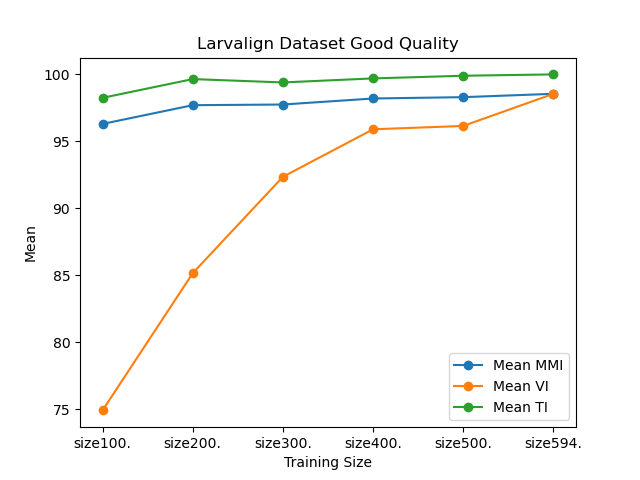
\includegraphics[width=0.9\columnwidth]{resources/ablation_size/size_effect_good.png}
		\caption{Graph showing the correlation between training set size and average MMI scores on the ``good" quality set of the \texttt{Larvalign dataset} using ``Cascaded Landmark Guided Voxelmorph methods".}
		\label{fig:size_effect_good}
	\end{figure}

	\begin{figure}[h!]
		\centering
		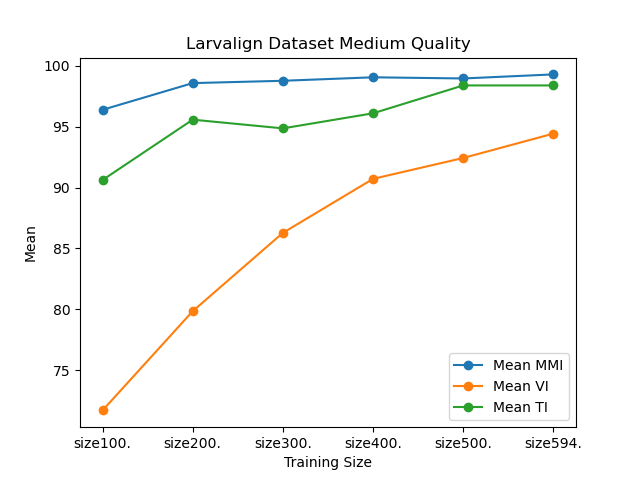
\includegraphics[width=0.9\columnwidth]{resources/ablation_size/size_effect_medium.png}
		\caption{Graph showing the correlation between training set size and average MMI scores on the ``medium" quality set of the \texttt{Larvalign dataset} using ``Cascaded Landmark Guided Voxelmorph methods".}
		\label{fig:size_effect_medium}
	\end{figure}

	\begin{figure}[h!]
		\centering
		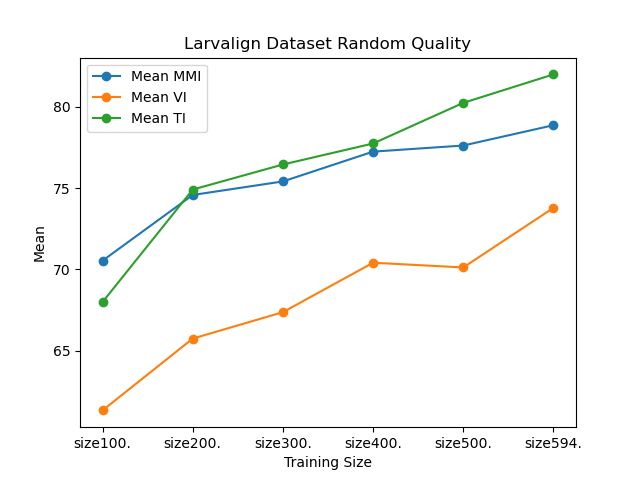
\includegraphics[width=0.9\columnwidth]{resources/ablation_size/size_effect_random.png}
		\caption{Graph showing the correlation between training set size and average MMI scores on the ``random" quality set of the \texttt{Larvalign dataset} using ``Cascaded Landmark Guided Voxelmorph methods".}
		\label{fig:size_effect_random}
	\end{figure}
	
	From the plots in the Figure~\ref{fig:size_effect_good}, Figure~\ref{fig:size_effect_medium}, and Figure~\ref{fig:size_effect_random} we can notice that the VNC Error Indicator (VI) tend to increase with an increase in the training set size for all ``good", ``medium", and ``random" quality images. However, for the Mattes Mutual Information (MMI) and Thoracic Nerve Error Indicator (TI) scores, the behavior is different.
	
	For good quality scans, the MMI and TI scores seem to reach a maximum score for a training set size of 400, while only increasing slightly from 300 to 400. For medium quality scans, the MMI and TI scores increase with increase in training set size and seems to be no improvement from training set size of 500 to 594 and the score is already closing in on the maximum value. However, we cannot tell for sure if it has saturated. Finally, for the random quality images, the MMI and TI scores increased almost at the same rate as the VI scores, continuously, and the maximum value reached is less than 80 for all the three scores.
	
	This trend suggests us that for random quality scans, where the quality of scans may not be good, a training size of more than 600 is definitely essential. The plots indicate that as the training size increases, the VI scores consistently improve. This suggests that for optimal registration accuracy in the lower regions of the ventral nerve cord (VNC), a larger training dataset is required. However, for other parts of the brain scans such as thoracic regions, comparitively smaller training dataset is sufficient.
	
	\begin{figure}[h!]
		\centering
		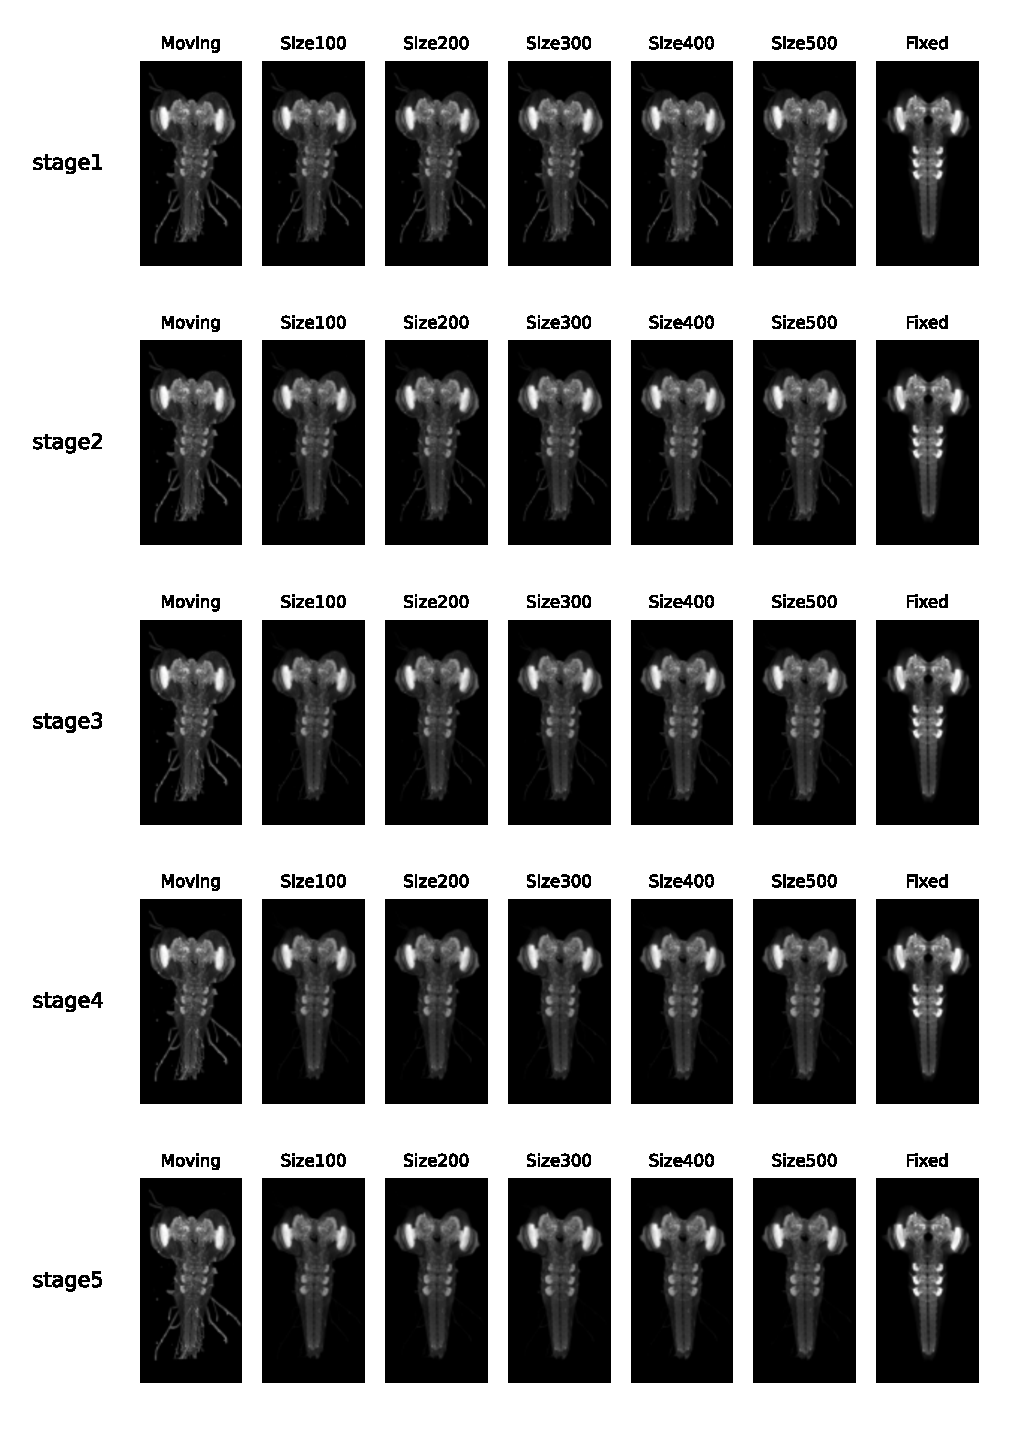
\includegraphics[width=\columnwidth]{resources/ablation_size/stage_vs_size_random.pdf}
		\caption{Illustrating the output at various stages of the cascaded network for a sample moving image from the ``random" quality set of the \texttt{Larvalign dataset}, as a function of different training set sizes, using the ``Cascaded Landmark Guided Voxelmorph" registration method.}
		\label{fig:stage_vs_size_random}
	\end{figure}
	
	Figure~\ref{fig:stage_vs_size_random} shows the output at each stage for a sample scan from the random quality set of the \texttt{Larvalign dataset} for models trained with different numbers of training set sizes. From the images in the rows, it is possible to see how the output at the end of each stage changed when the same model was trained with a different number of training samples. Our main interest is in the last row, i.e., stage 5, where the final registered image is output. Looking at the images in this row, we can see how the registration improves with increasing training size. This is a visual inspection of the effect of training size on performance in addition to the graphs in Figure~\ref{fig:size_effect_good}, Figure~\ref{fig:size_effect_medium}, and Figure~\ref{fig:size_effect_random}, which provide a clear understanding of the relationship between training data size and model performance. Also, you can examine the images column by column and see how the results changed at each stage for a particular model.
	
	\subsection{Mean Squared Error as similarity (loss) function}
	Ablation study in the context of loss functions can be used to determine which loss function is most effective for a given task when more than one loss functions seems reasonable. In our case, in addition to the Normalized Cross-Correlation (NCC) similarity function, we also checked the Mean Squared Error (MSE) to compute the similarity between the registered and fixed image.
	
	When using the Mean Squared Error (MSE) method, the model attempts to reproduce the fixed image exactly as it is. Unlike the Normalized Cross-Correlation (NCC) method, MSE focused on creating a perfect replica of the fixed image. However, this can lead to structures that appear artificial or blurred in the reproduced image as seen in Figure~\ref{fig:ablation_loss}.
	
	\begin{figure}[h!]
		\centering
		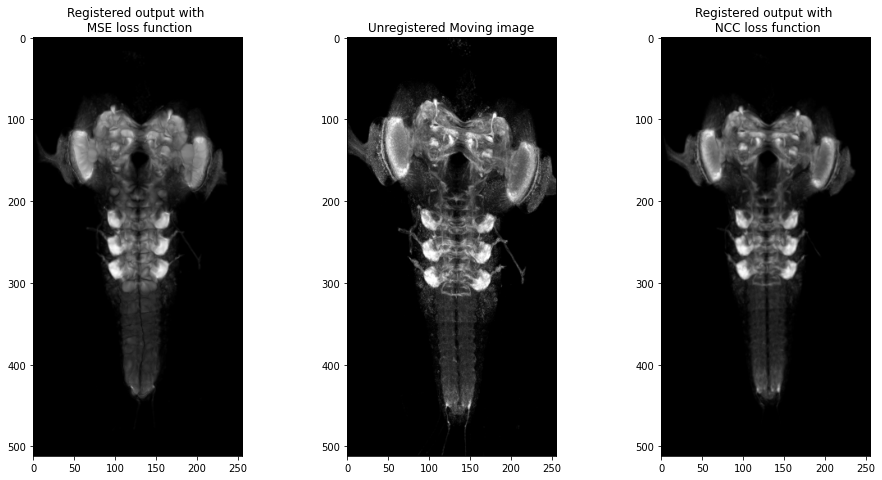
\includegraphics[width=0.9\columnwidth]{resources/ablation_loss/ablation_loss.png}
		\caption{Comparison of registration results using MSE (left) and NCC (right) methods. The MSE method tries to create an exact replica of the fixed image, however, this can result in artificial or blurred structures as seen at the thoracic region.}
		\label{fig:ablation_loss}
	\end{figure}
		
	\chapter{Discussion}\label{chapter:discussion}
	The goal of this chapter is to provide a clear and concise summary of the key findings of the research, and to interpret and discuss their significance in relation to the research question of whether deep learning is a fast and robust method for image registration compared to the traditional way of performing image registration.
	
	\section{Quantitative Assessment on Landmark Registration Error (LRE)}
	Landmark registration errors (LRE) were computed on ``Cascaded Vanilla Voxelmorph", ``Cascaded Landmark Guided Voxelmorph", and \textit{larvalign} registered output scans from the ``medium" quality set in \texttt{Larvalign dataset}. The Table~\ref{table:lre} summarizes the distribution of these errors across these three registration methods and we can notice that \textit{larvalign} method clearly has a better score than ``Cascaded Vanilla Voxelmorph" or ``Cascaded Landmark Guided Voxelmorph" in all respects. 
	
	\begin{figure}[h!]
		\centering
		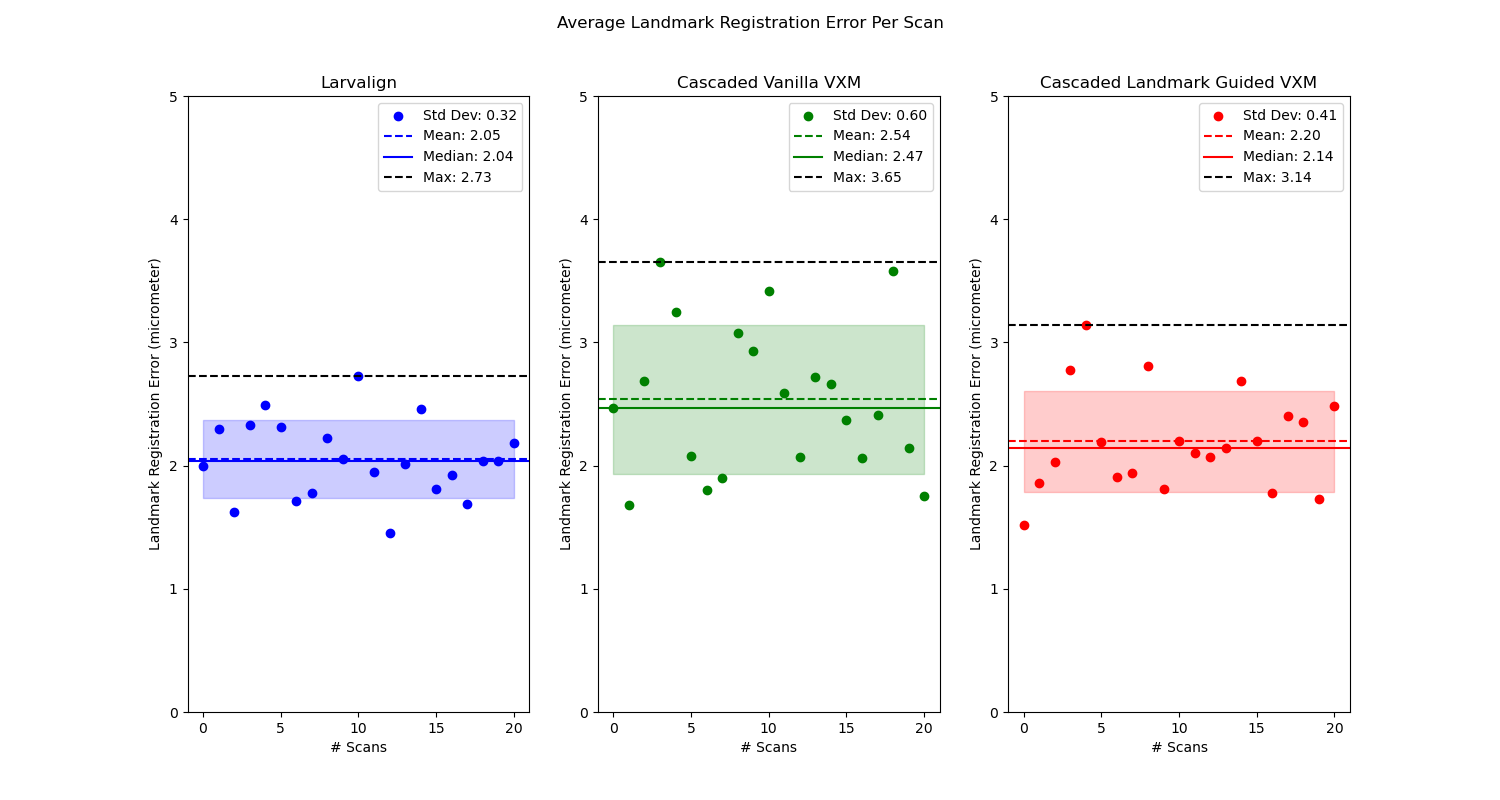
\includegraphics[width=0.9\columnwidth]{resources/chapter5_fresh/stats_per_scan_output/Stats_Per_Landmark.png}
		\caption{Landmark registration error (LRE) were averaged per registration on the ``medium" quality \texttt{Larvalign dataset} for all three approaches and the average error distribution is plotted.}
		\label{fig:mean_stats_per_scan}
	\end{figure}

	\begin{table}[h!]
		\centering
		\begin{tabular}{lcc}
\hline
 Method   & Average Mean LRE (mm) & Average Std Dev LRE (mm) \\ \hline \hline
 Larvalign & \textbf{2.1}               & \textbf{1.02}                 \\
 Method3   & 2.64              & 1.47                 \\
 Method4   & 2.29              & 1.07                 \\
\hline
\end{tabular}
		\caption{Summary of landmark registration error (LRE) averaged per registration and the mean error, the median error, the max error, and the corresponding standard deviation were calculated on the ``medium" quality scans of \texttt{Larvalign dataset} across all 3 approaches.}
		\label{table:lre}
	\end{table}
	
	Although the summary values in table~\ref{table:lre} make it appear that all three registration methods perform almost equally well in terms of landmark registration error (LRE), the plot of the error distribution in Figure~\ref{fig:mean_stats_per_scan} shows that the landmark registration error (LRE) is quite wide for the ``Cascaded Vanilla Voxelmorph" method. And both the \textit{larvalign} and the ``Cascaded Landmark Guided Voxelmorph" methods have comparable statistical values and error distributions.
	
	Though the maximum error for the ``Cascaded Landmark Guided Voxelmorph" method is larger than for the \textit{larvalign} method, the difference is only 0.41 \textmu m. This is acceptable because we know from the \textit{larvalign} \cite{larvalign} paper that the diameter of anatomical structures at the selected landmarks - often nerve entry points, ranges from 2-8 \textmu m, with more than 50\% of the structures having a diameter of 5 \textmu m. In addition, assessment of intra-rater variability in landmark annotation by the same neurobiologist as shown that there is a mean intra-rater variance of 2.0 $\pm$ 1.2 \textmu m and a maximum intra-rater variance of 3.5 $\pm$ 1.8 \textmu m \cite{larvalign}. Considering these information, the difference of less than half a micrometer is quite negligible.
	
	\section{Quantitative Assessment on Mattes Mutual Information Scores}
	Mattes Mutual Information scores in the region of the VNC, thoracic nerve entry points, and throughout the image were measured for all images (``good," ``medium," and ``random") from the \texttt{Larvalign dataset}. The following Table~\ref{table:quality_good}, Table~\ref{table:quality_medium}, table~\ref{table:quality_random} contains the summary scores averaged over the ``good," ``medium," and ``random" quality images.
	
	\begin{table}[h!]
		\centering
		\begin{adjustbox}{width=0.6\columnwidth}
\begin{tabular}{lccc}
\hline
 Methods  & MMI   & VI    & TI  \\ \hline \hline
 Larvalign & 88.25 & 96.2  & 78  \\
 Cascaded Vanilla VXM  & 98.50 & 91.65 & 100 \\
 Cascaded Landmark Guided VXM  & \textbf{98.55} & \textbf{98.55} & \textbf{100} \\
\hline
\end{tabular}
\end{adjustbox}
		\caption{Average MMI, VI, and TI errors across all the ``good" quality images in \texttt{Larvalign dataset} for each method.}
		\label{table:quality_good}
	\end{table}
	
	\begin{table}[h!]
		\centering
		\begin{tabular}{lccc}
\hline
 Methods  & MMI   & VI    & TI    \\ \hline \hline
 Larvalign & 86.29 & 93.57 & 75.19 \\
 Cascaded Vanilla VXM  & \textbf{99.33} & 86.05 & \textbf{99.05} \\
 Cascaded Landmark Guided VXM  & 99.24 & \textbf{94.33} & 98.52 \\
\hline
\end{tabular}
		\caption{Average MMI, VI, and TI errors across all the ``medium" quality images in \texttt{Larvalign dataset} for each method.}
		\label{table:quality_medium}
	\end{table}
	
	\begin{table}[h!]
		\centering
		\begin{adjustbox}{width=0.6\linewidth}
\begin{tabular}{lccc}
\hline
 Methods  & MMI   & VI    & TI    \\ \hline \hline
 Larvalign & 61.29 & 69.00 & 62.88 \\
 Cascaded Vanilla VXM  & \textbf{79.79}  & 67.13 & \textbf{83.29} \\
 Cascaded Landmark Guided VXM  & 78.71 & \textbf{73.67} & 82.04 \\
\hline
\end{tabular}
\end{adjustbox}
		\caption{Average MMI, VI, and TI errors across all the ``random" quality images in \texttt{Larvalign dataset} for each method.}
		\label{table:quality_random}
	\end{table}

	From the tables, we can see that both methods, ``Cascaded Vanilla Voxelmorph" and ``Cascaded Landmark Guided Voxelmorph", significantly outperform the \textit{larvalign} method. More specifically, we can see that the VI score for ``Cascaded Landmark Guided Voxelmorph" is better for all image qualities because we specifically introduced landmark points to control the registration process. This is another proof that adding landmark information leads to better performance.
	
	\section{Landmark Registration Error at Ventral Nerve Cord (VNC)}
	In this section, we will discuss the improvements seen in the accuracy of registration at the lower tip of ventral nerve cord (VNC) upon adding the landmarks into the training as auxiliary information. Figure~\ref{fig:vnc} shows 7 landmarks that were identified by the biologists in \textit{larvalign} paper.
	
	\begin{figure}[h!]
		\centering
		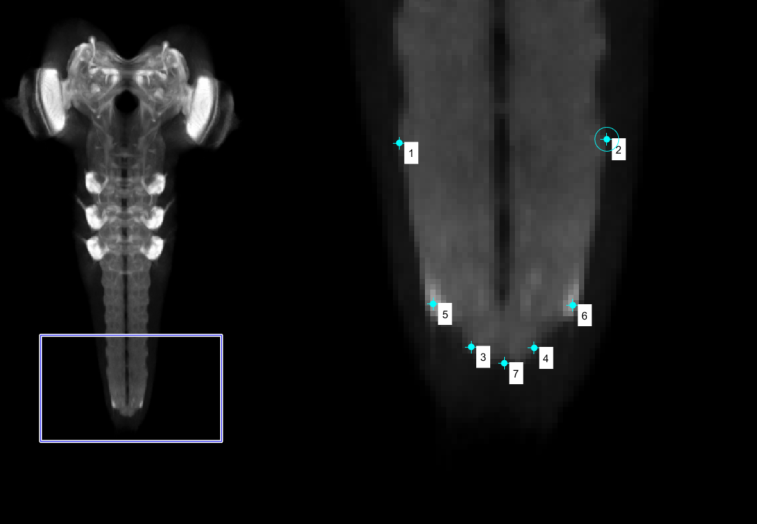
\includegraphics[width=0.9\columnwidth]{resources/chapter7/VNC.png}
		\caption{Lower ventral nerve cord (VNC) region in the template brain of Drosophila larva and the associated landmark points in the region. (1,2) are the right/left A8 nerve entry points, (3,4) are the right/left A6 nerve entry points, (5,6) are the right/left A7 nerve entry points, and (7) is the end of ventral nerve cord.}
		\label{fig:vnc}
	\end{figure}
	
	From Figure~\ref{fig:landmark1}, Figure~\ref{fig:landmark7}, Figure~\ref{fig:landmark15}, Figure~\ref{fig:landmark22}, Figure~\ref{fig:landmark24}, Figure~\ref{fig:landmark26} and Figure~\ref{fig:landmark27}, it can be clearly seen that the landmark registration error (LRE) in the VNC region is high for the ``Cascaded Vanilla Voxelmorph" method compared to the \textit{larvalign} method or the ``Cascaded Landmark Guided Voxelmorph" method. Also, it is clearly evident that adding landmark points in the VNC region helped the network perform better registration than ``Cascaded Vanilla Voxelmorph".
	
	Because the labeling of the entry points of ``right/left A6 nerve entry" and ``right/left A8 nerve entry" were not accurate for the reasons mentioned in section~\nameref{subsec:landmark_distance} in chapter~\nameref{chapter:results}, we will consider only the entry points of ``right/left A7 nerve entry" and ``end point of the ventral nerve cord" for analysis. For convenience, they are represented here again as Figure~\ref{fig:re_landmark22}, Figure~\ref{fig:re_landmark27}, and Figure~\ref{fig:re_landmark15}.
	
	\begin{figure}[h!]
		\centering
		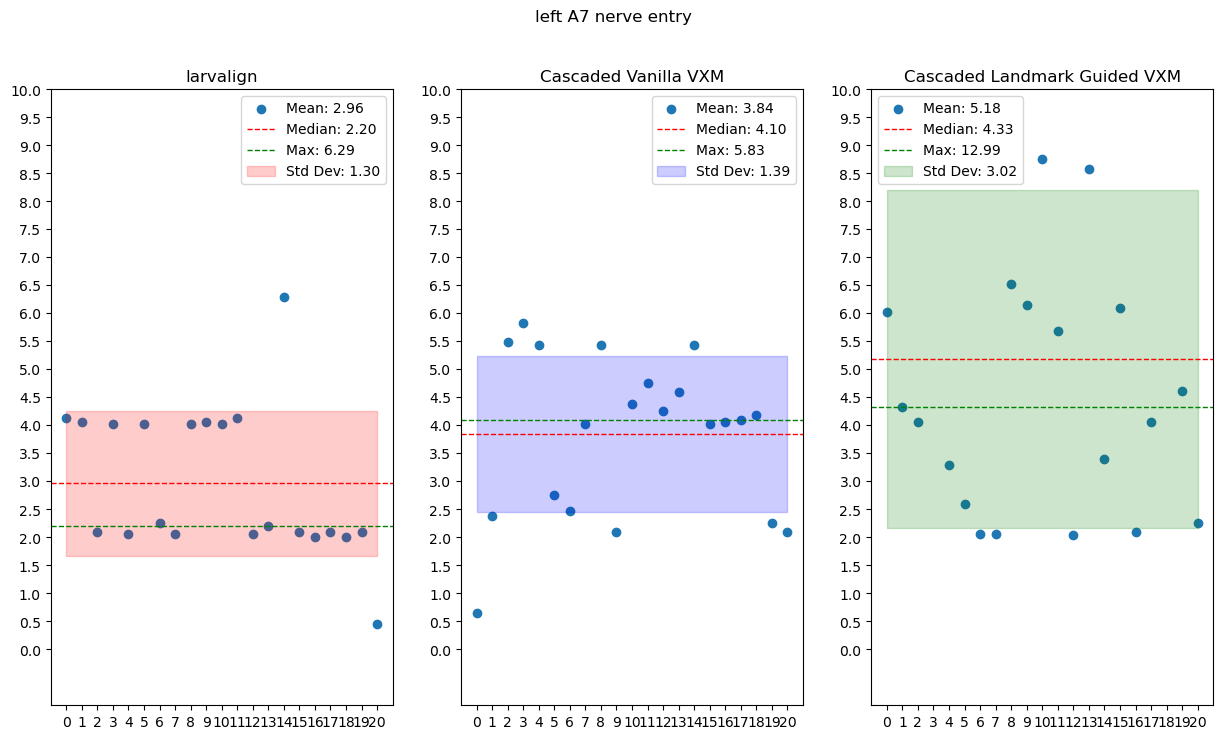
\includegraphics[width=0.9\columnwidth]{resources/chapter5_fresh/output/left A7 nerve entry.png}
		\caption{LRE plot distribution for ``left A7 nerve entry" landmark point measured across different scans from the ``medium" quality \texttt{Larvalign dataset}.}
		\label{fig:re_landmark22}
	\end{figure}
	
	\begin{figure}[h!]
		\centering
		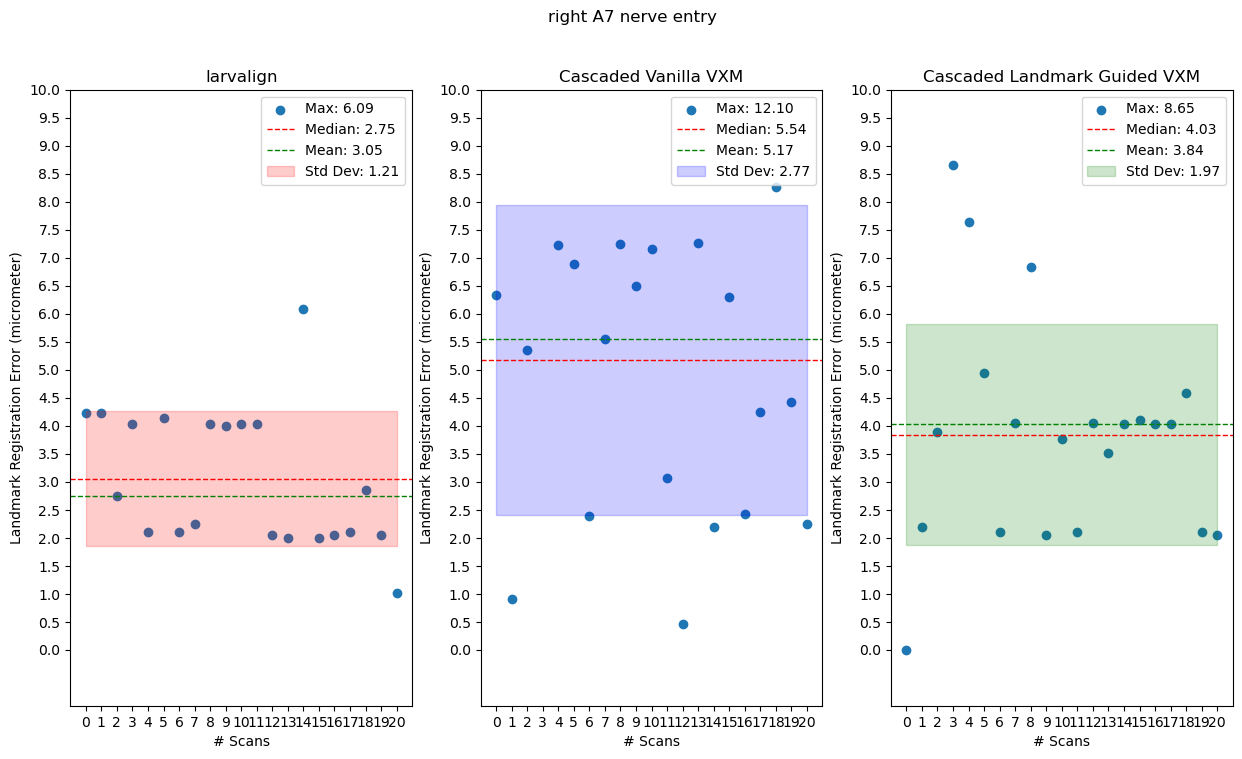
\includegraphics[width=0.9\columnwidth]{resources/chapter5_fresh/output/right A7 nerve entry.png}
		\caption{LRE plot distribution for ``right A7 nerve entry" landmark point measured across different scans from the ``medium" quality \texttt{Larvalign dataset}.}
		\label{fig:re_landmark27}
	\end{figure}
	
	\begin{figure}[h!]
		\centering
		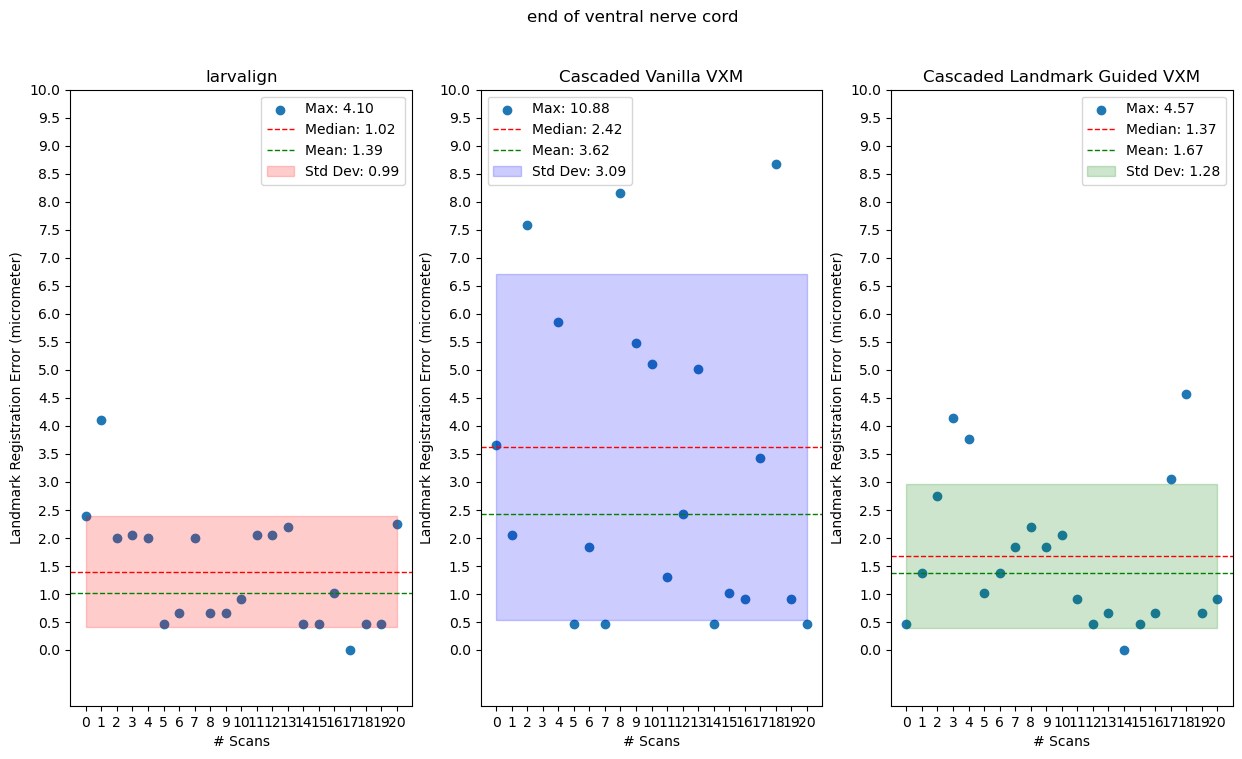
\includegraphics[width=0.9\columnwidth]{resources/chapter5_fresh/output/end of ventral nerve cord.png}
		\caption{LRE plot distribution for ``end of ventral nerve cord" landmark point measured across different scans from the ``medium" quality \texttt{Larvalign dataset}.}
		\label{fig:re_landmark15}
	\end{figure}
	
	The ``Cascaded Vanilla Voxelmorph" method is the least accurate of the three methods when it comes to accurately registering the landmark points at the lower tip of the VNC.
	
	Table~\ref{table:vnc_lre} indicate that the average deviation in landmark registration error (LRE) at the VNC landmark points is better for \textit{larvalign} method. However, \emph{larvalign} is better only by less than 1 \textmu m, where as the intra-rater variance itself is about 2 \textmu m.
	
	We can analyze the Figure~\ref{fig:re_landmark22}, Figure~\ref{fig:re_landmark27}, and Figure~\ref{fig:re_landmark15} more closely and notice that brain scans (4) and (5) have large outliers in landmark registration errors at all the 3 landmark points for ``Cascaded Landmark Guided Voxelmorph" method and the for our reference, Table~\ref{table:brain45_lre} captures this absolute error between the two registration approaches at the specific landmarks.
	
	\begin{table}[H]
		\centering
		\begin{adjustbox}{width=\textwidth}
	\begin{tabular}{lccc}
		& \multicolumn{1}{l}{} & \multicolumn{1}{l}{} & \multicolumn{1}{l}{} \\ \hline
		\multicolumn{1}{|l|}{Method} & \multicolumn{1}{c|}{\begin{tabular}[c]{@{}c@{}}Right A7 Nerve Entry\\ LRE (\textmu m)\end{tabular}} & \multicolumn{1}{c|}{\begin{tabular}[c]{@{}c@{}}Left A7 Nerve Entry\\ LRE (\textmu m)\end{tabular}} & \multicolumn{1}{c|}{\begin{tabular}[c]{@{}c@{}}End of Ventral Nerve\\ Cord LRE (\textmu m)\end{tabular}} \\ \hline
		\multicolumn{1}{|l|}{} & \multicolumn{1}{c|}{} & \multicolumn{1}{c|}{} & \multicolumn{1}{c|}{} \\
		\multicolumn{1}{|l|}{Larvalign} & \multicolumn{1}{c|}{\textbf{3.05 $\pm$ 1.21}} & \multicolumn{1}{c|}{\textbf{2.96 $\pm$ 1.30}} & \multicolumn{1}{c|}{\textbf{1.39 $\pm$ 0.99}} \\
		\multicolumn{1}{|l|}{Cascaded Landmark Guided VXM} & \multicolumn{1}{c|}{3.84 $\pm$ 1.97} & \multicolumn{1}{c|}{3.84 $\pm$ 1.39} & \multicolumn{1}{c|}{1.67 $\pm$ 1.28} \\ \hline \hline
		\multicolumn{1}{|l|}{Difference in Mean} & \multicolumn{1}{c|}{0.79} & \multicolumn{1}{c|}{0.88} & \multicolumn{1}{c|}{0.28} \\ \hline
	\end{tabular}
\end{adjustbox}
		\caption{Average deviation in landmark registration error (LRE) for the entry points of the A7 right/left nerve and the end of the ventral nerve cord on all scans from ``medium" quality set in the \texttt{Larvalign dataset} for the \textit{larvalign} and ``Cascaded Landmark Guided Voxelmorph" methods.}
		\label{table:vnc_lre}
	\end{table}
	
	\begin{table}[H]
		\centering
		\begin{adjustbox}{width=\linewidth}
	\begin{tabular}{lcclcc}
		& \multicolumn{1}{l}{} & \multicolumn{1}{l}{} &  & \multicolumn{1}{l}{} & \multicolumn{1}{l}{} \\ \hline
		\multicolumn{1}{|c|}{\multirow{2}{*}{\textbf{Landmark Name}}} & \multicolumn{2}{c|}{\textbf{Brain Scan 4}} & \multicolumn{1}{l|}{} & \multicolumn{2}{c|}{\textbf{Brain Scan 5}} \\ \cline{2-6} 
		\multicolumn{1}{|c|}{} & Larvalign & \multicolumn{1}{c|}{\begin{tabular}[c]{@{}c@{}}Cascaded Landmark\\ Guided VXM\end{tabular}} & \multicolumn{1}{l|}{} & Larvalign & \multicolumn{1}{c|}{\begin{tabular}[c]{@{}c@{}}Cascaded Landmark\\ Guided VXM\end{tabular}} \\ \hline
		\multicolumn{1}{|l|}{} & \multicolumn{1}{l}{} & \multicolumn{1}{l|}{} & \multicolumn{1}{l|}{} & \multicolumn{1}{l}{} & \multicolumn{1}{l|}{} \\
		\multicolumn{1}{|l|}{Right A7 Nerve Entry Point LRE (\textmu m)} & 4.03 & \multicolumn{1}{c|}{8.65} & \multicolumn{1}{c|}{} & 2.10 & \multicolumn{1}{c|}{7.63} \\
		\multicolumn{1}{|l|}{Left A7 Nerve Entry Point LRE (\textmu m)} & 4.03 & \multicolumn{1}{c|}{5.83} & \multicolumn{1}{c|}{} & 2.05 & \multicolumn{1}{c|}{5.43} \\
		\multicolumn{1}{|l|}{End of Ventral Nerve Cord LRE (\textmu m)} & 2.05 & \multicolumn{1}{c|}{4.14} & \multicolumn{1}{c|}{} & 2.00 & \multicolumn{1}{c|}{3.77} \\ \hline
	\end{tabular}
\end{adjustbox}

		\caption{One-to-one comparison of landmark registration error (LRE) for Brain Scan 4 and 5 for \textit{larvalign}-registered output and ``Cascaded Landmark Guided Voxelmorph"-registered output at landmark locations ``Right/Left A7 Nerve Entry Points" and ``End of Ventral Nerve Cord".}
		\label{table:brain45_lre}
	\end{table}
	
	Figures~\ref{fig:14c08b_overlay} and \ref{fig:14c08c_overlay} show registered brain scans (4) and (5) overlaid with the template to show how poor or alright the registration is.

	The registered image of ``Cascaded Landmark Guided Voxelmorph" has not perfectly registered, yes. But, it needs to noted that the model was trained on \texttt{Janelia dataset} and tested on \texttt{Larvalign dataset}. Training explicitly on \texttt{Larvalign dataset} and testing on the same dataset would give better results.
	
	It is important to mention that the landmark registration error (LRE) can also be due to the presence of structures in different slice order. For example, the overlay with the \textit{larvalign}-registered output in Figure~\ref{fig:14c08b_overlay} appears to be very perfect at the ``end of ventral nerve cord" landmark. However, the error is still 2.05 \textmu m because the structure appears at slice number 36 in the fixed image, whereas the same structure appears at slice number 34 in the registered image. So sometimes the registration error can be due to the structures being at a different depth.
	
	\begin{figure}[h!]
		\centering
		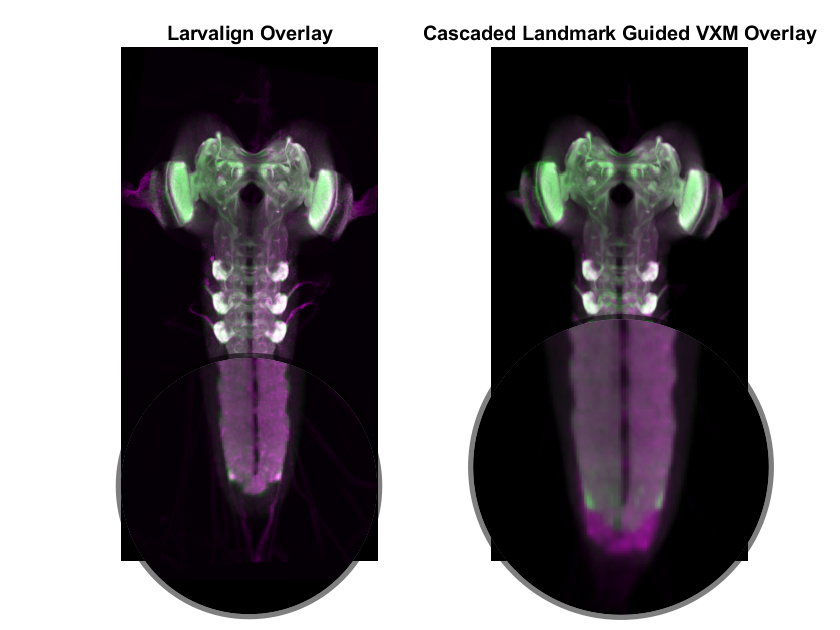
\includegraphics[width=0.7\columnwidth]{resources/chapter7/LRE_Visual/14c08b_overlay_zoomed.png}
		\caption{Focused overlay of the maximum intensity projection of the fixed image with the maximum intensity projection of the registered \textit{larvalign} output and the maximum intensity projection of the registered ``Cascaded Landmark Guided Voxelmorph" output for Brain Scan (4).}
		\label{fig:14c08b_overlay}
	\end{figure}
	
	\begin{figure}[h!]
		\centering
		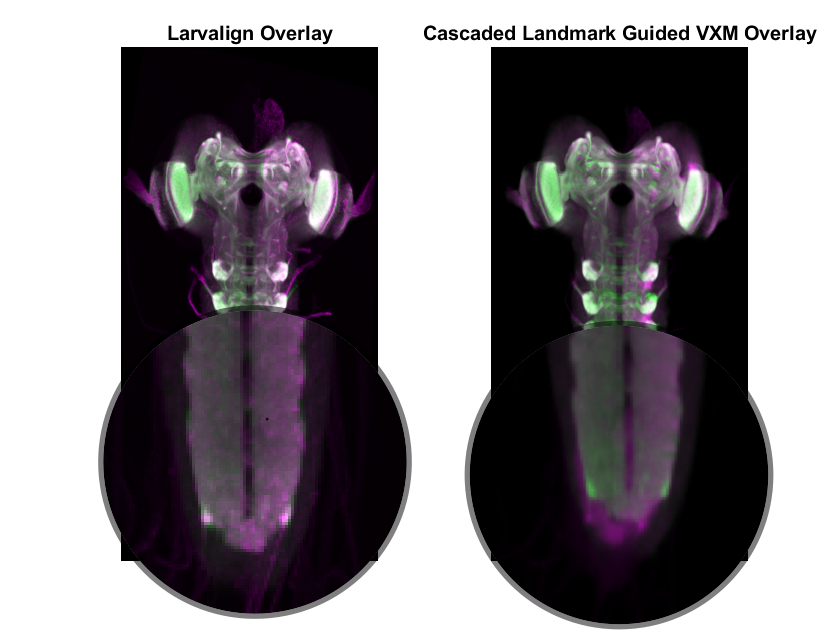
\includegraphics[width=0.7\columnwidth]{resources/chapter7/LRE_Visual/14c08c_overlay_zoomed.png}
		\caption{Focused overlay of the maximum intensity projection of the fixed image with the maximum intensity projection of the registered \textit{larvalign} output and the maximum intensity projection of the registered ``Cascaded Landmark Guided Voxelmorph" output for Brain Scan (5).}
		\label{fig:14c08c_overlay}
	\end{figure}
	
	\newpage
	\section{Cascaded Landmark Guided Voxelmorph's ability to learn from mistakes.}
	One of the key features we wanted to find out was whether the Deep Learning Neural Network could learn from its mistakes and not make the same registration error as \textit{larvalign}. In \emph{larvalign}'s work, three erroneous registrations were shown in Fig. 3 of \textit{larvalign}'s work, and one such registrations was also mentioned in the section~\nameref{sec:motivation} in chapter~\nameref{chap:intro}. These brain scans are part of the ``random" quality set of the \texttt{Larvalign dataset}. Figure~\ref{fig:larvalign failure 1}, Figure~\ref{fig:larvalign failure 2}, and Figure~\ref{fig:larvalign failure 3} shows an overlay between the \textit{larvalign} registered output and ``Cascaded Landmark Guided Voxelmorph" registered output.
	
	One can notice the presence of magenta structures at the lower end of the Ventral Nerve Cord in the \textit{larvalign} registered outputs. These magenta structures are the structures where the registration has failed. In contrast, the corresponding output for the ``Cascaded Landmark Guided Voxelmorph" registered output shows no such magenta structures, and there is nice overlap between the fixed image and the registered image. Though, in the previous sections we saw that landmark registration error (LRE) for \textit{larvalign} is better, ``Cascaded Landmark Guided Voxelmorph" is able to generalize better and handle the scenarios where \textit{larvalign} fails.
	
	\begin{figure}[h!]
		\centering
		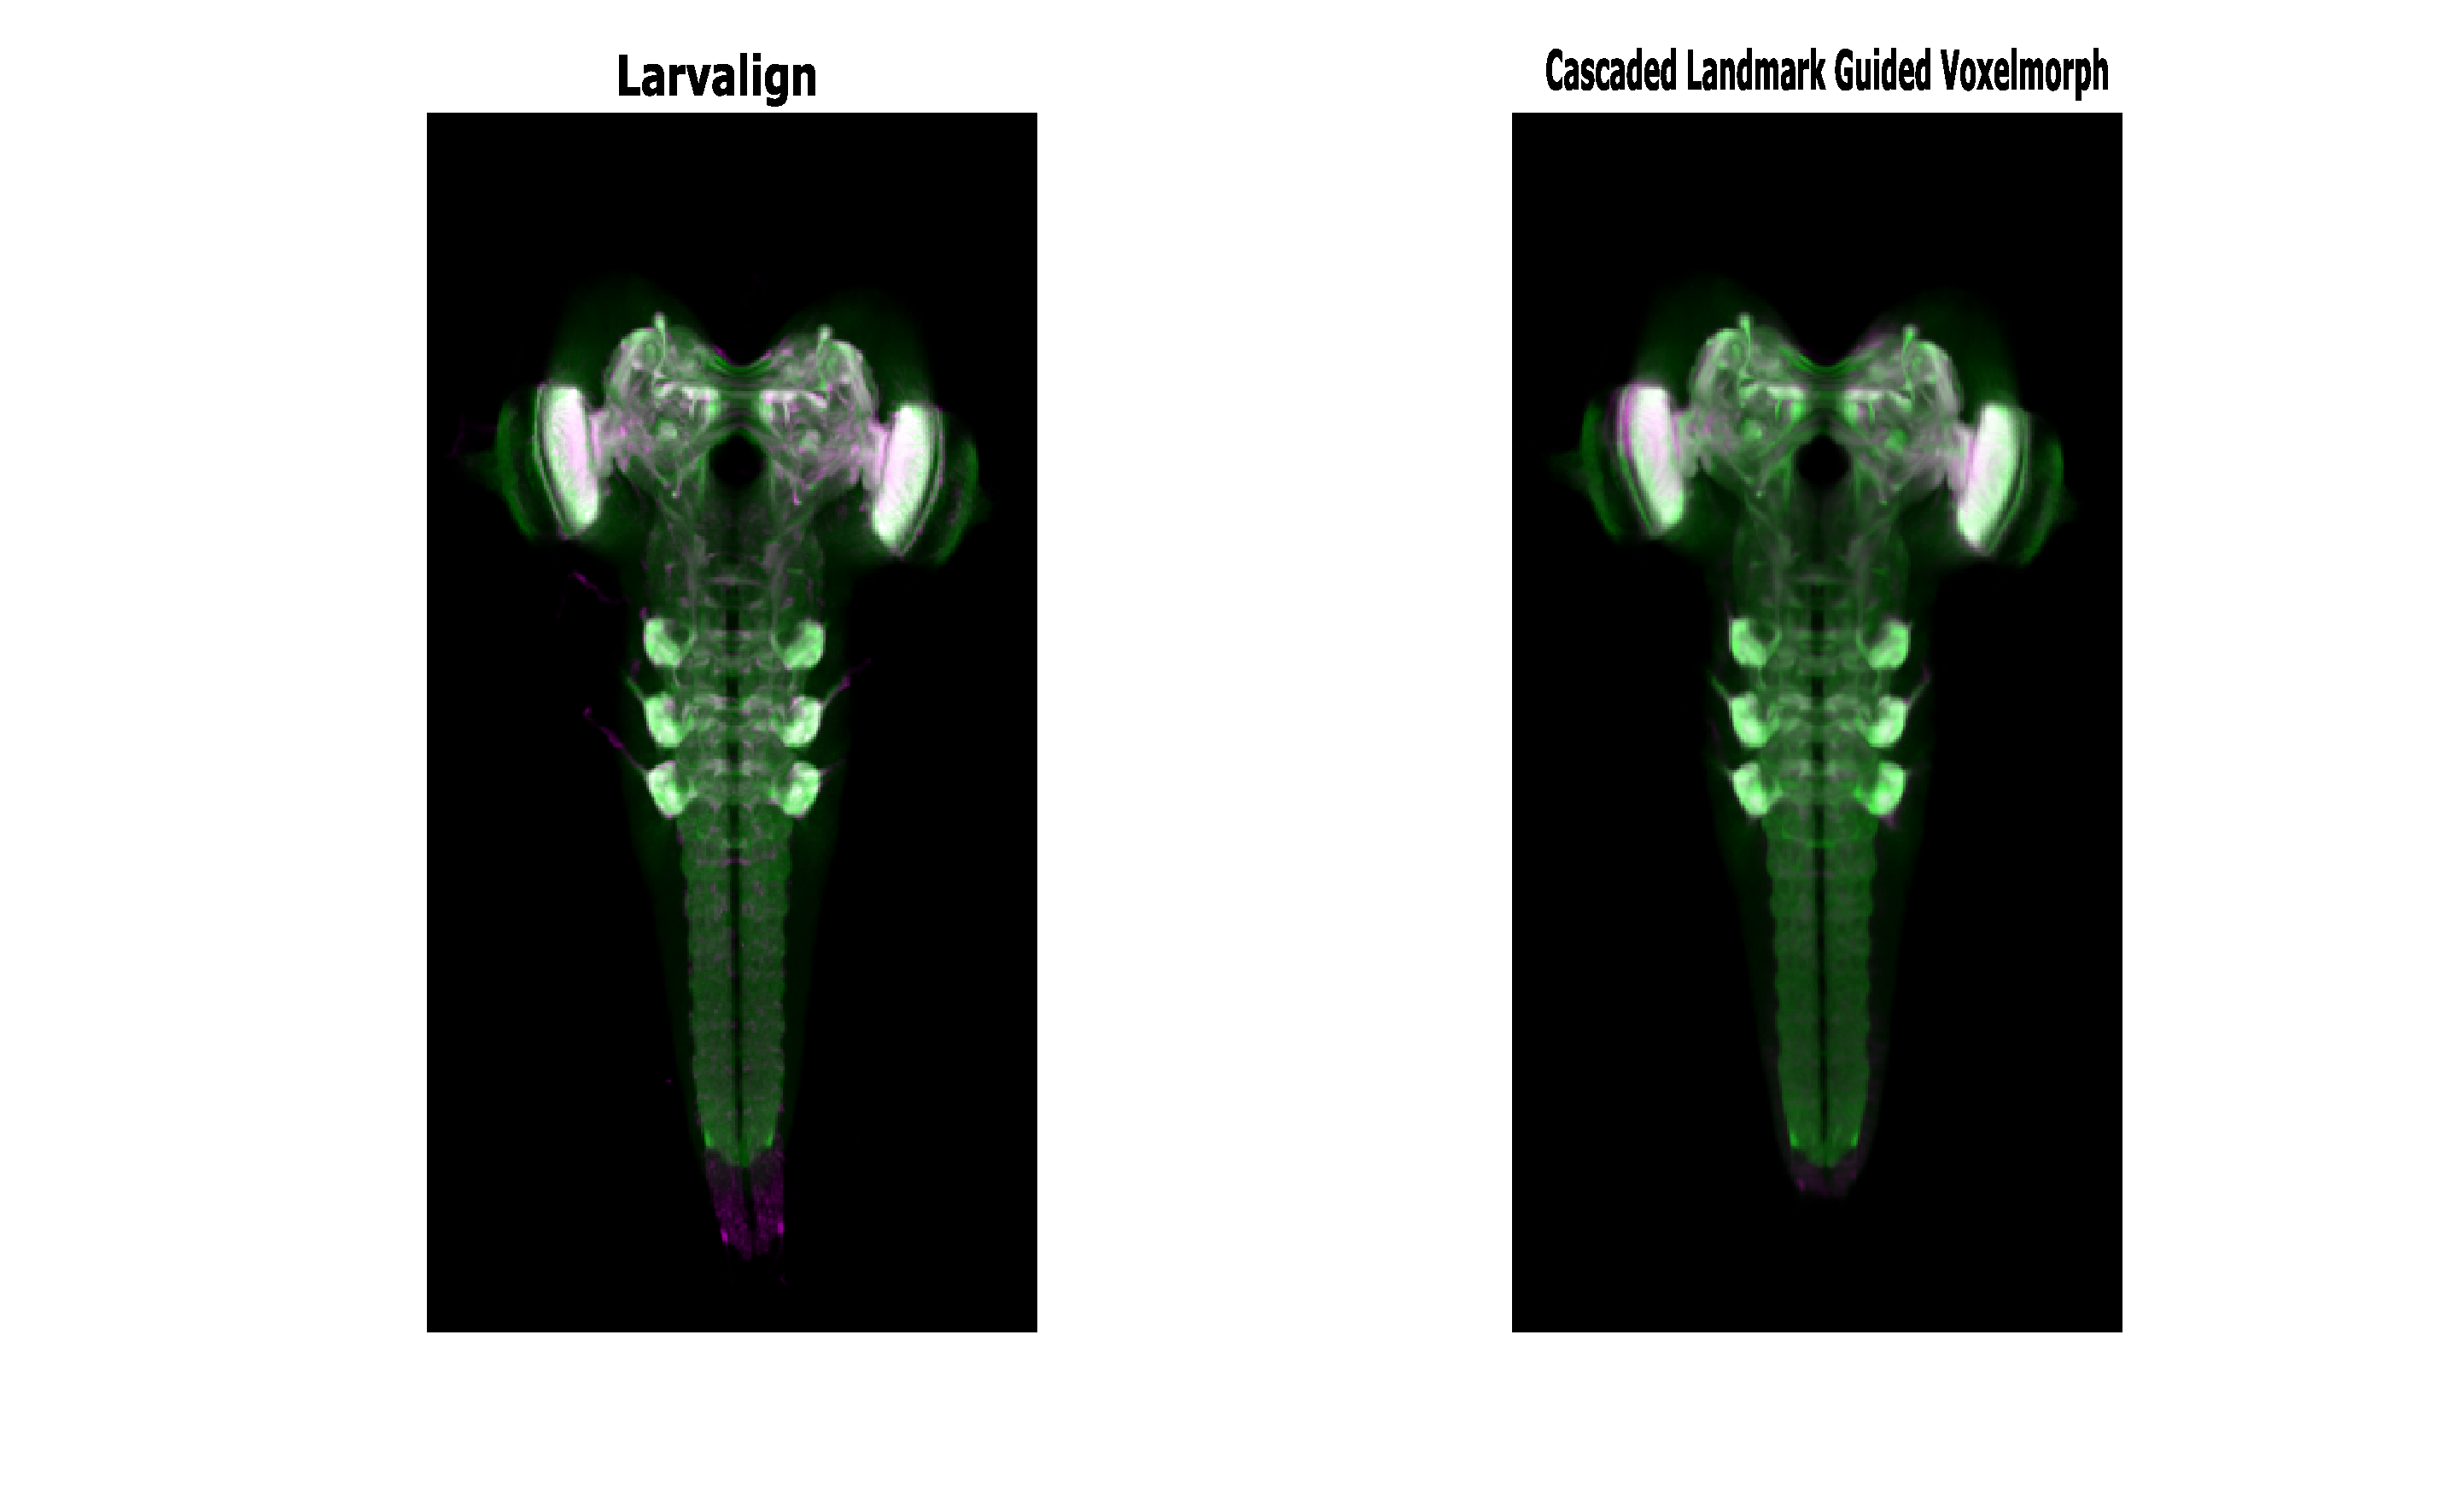
\includegraphics[width=0.9\columnwidth]{resources/chapter7/LRE_Visual/failure1.pdf}
		\caption{Overlay of the maximum intensity projection of the fixed image with the maximum intensity projection of the registered \textit{larvalign} output and the maximum intensity projection of the registered ``Cascaded Landmark Guided Voxelmorph" output for \texttt{larvalign failure 1}.}
		\label{fig:larvalign failure 1}
	\end{figure}
	
	\begin{figure}[h!]
		\centering
		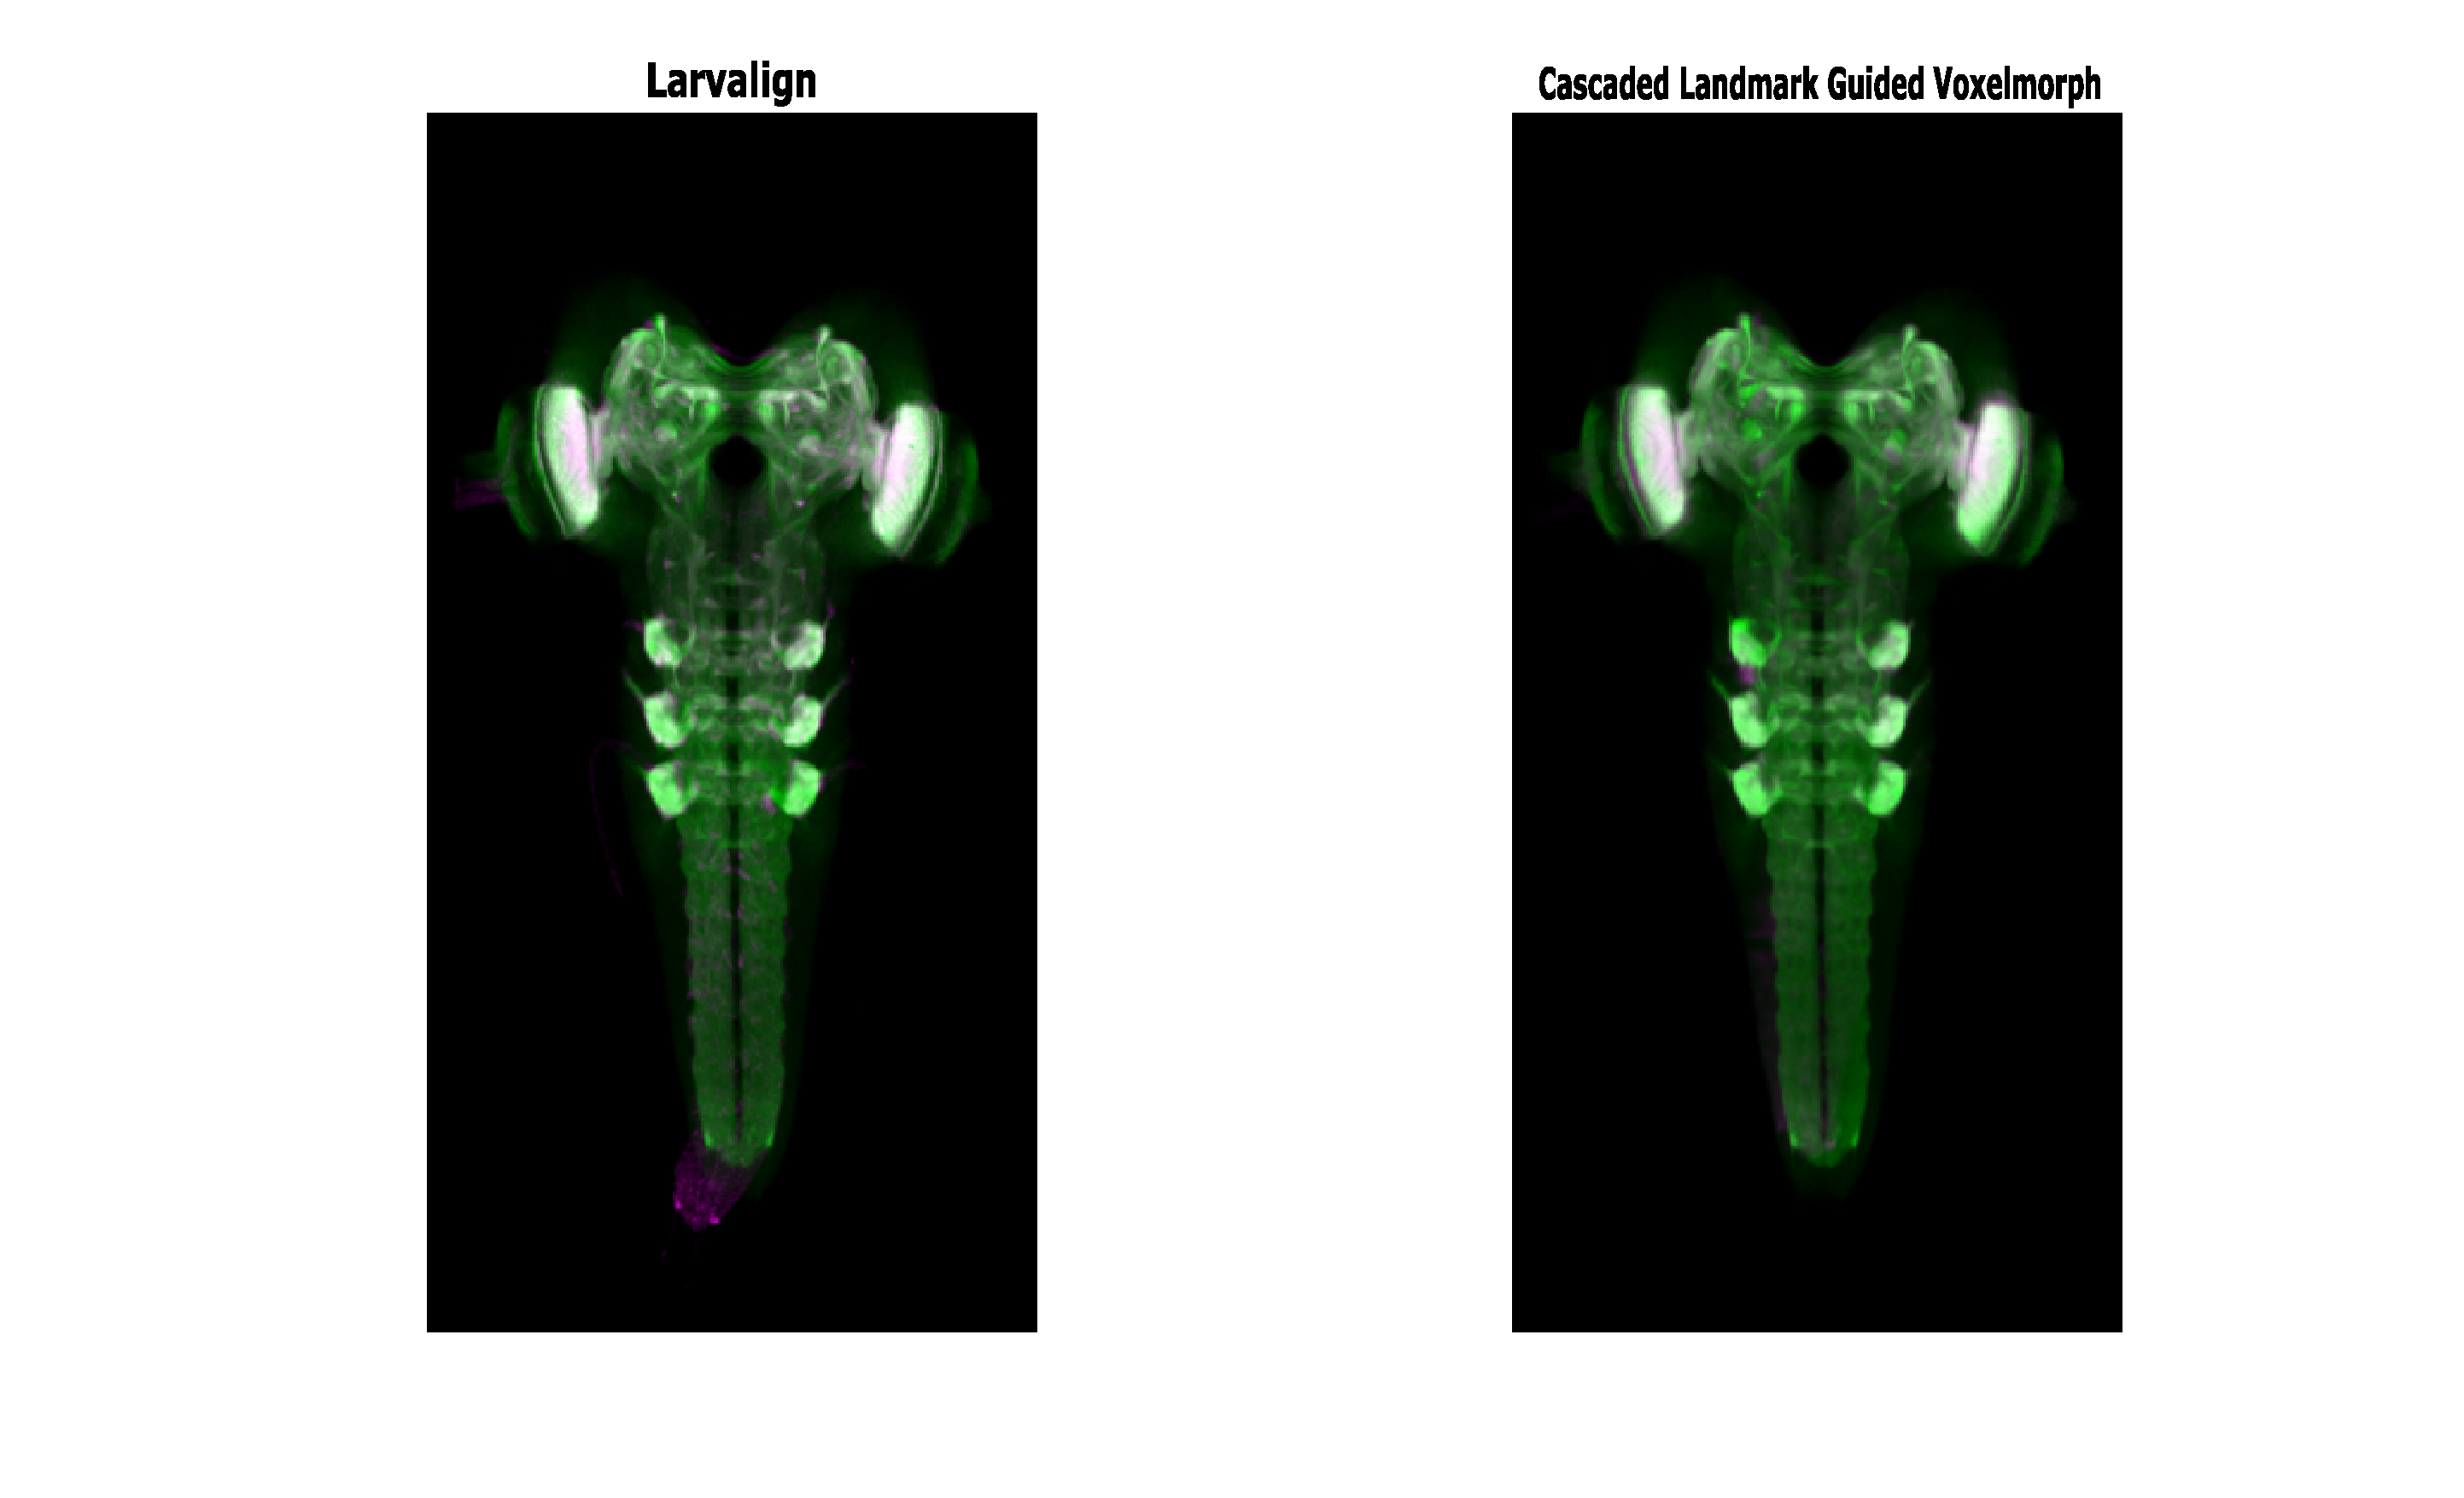
\includegraphics[width=0.9\columnwidth]{resources/chapter7/LRE_Visual/failure2.pdf}
		\caption{Overlay of the maximum intensity projection of the fixed image with the maximum intensity projection of the registered \textit{larvalign} output and the maximum intensity projection of the registered ``Cascaded Landmark Guided Voxelmorph" output for \texttt{larvalign failure 2}.}
		\label{fig:larvalign failure 2}
	\end{figure}

	\begin{figure}[h!]
		\centering
		\includegraphics[width=0.9\columnwidth]{resources/chapter7/LRE_Visual/failure3.pdf}
		\caption{Overlay of the maximum intensity projection of the fixed image with the maximum intensity projection of the registered \textit{larvalign} output and the maximum intensity projection of the registered ``Cascaded Landmark Guided Voxelmorph" output for \texttt{larvalign failure 3}.}
		\label{fig:larvalign failure 3}
	\end{figure}
	
	\section{Cascaded Landmark Guided Voxelmorph produces blurry registered output.}
	The registration process using ``Cascaded Landmark Guided Voxelmorph" was successful, but the registered output image was found to be blurred. Further analysis revealed that the blurriness was due to the Voxelmorph model causing blur at each stage of the output. As multiple stages were used in cascade, at the final output, the effect was compounded. To investigate the cause of the blurring in a single stage of the Voxelmorph model, we suspected that anisotropy in the images, both in terms of voxel resolution and the number of voxels in the x, y, and z directions, might be the cause. The scan resolution used in our training data was \texttt{256x512x64} and the voxel resolution was \texttt{0.45x0.45x2.0} \textmu m, but the image resolution used in the Voxelmorph research paper was \texttt{160x192x224} and had a voxel resolution of \texttt{1} mm in all directions.
	
	\begin{figure}[H]
		\centering
		\includegraphics[width=0.7\columnwidth]{resources/discussion/anisotropic_effect/Result_1.png}
		\caption{Maximum intensity projection of the outputs from the Isotropic model (a) and Anisotropic model (b). (c) represents the pixel-wise difference between the two images.}
		\label{fig:anisotropisum_result1}
	\end{figure}

	To test our hypothesis, we created two new training datasets - an isotropic and an anisotropic training dataset. The isotropic training dataset contained scans with a resolution of \texttt{128x128x128} in terms of the number of voxels, and the anisotropic training dataset contained scans with a resolution of \texttt{128x128x32} in terms of the number of voxels. We now trained two models - model\_isotropic and model\_anisotropic - independently with isotropic and anisotropic datasets for \texttt{50} epochs each and performed test registration with one of the scans.
	
	Since the output registered images from both the models were of the size \texttt{128x128} in xy directions, it was hard to visually say if there was any blurriness induced in the model's output trained on anisotropic scans. To answer it, we did the following analysis. We made the assumption that the output of the model\_anisotropic is a blurrier version of the output of the model\_isotropic. If our assumption is true then the difference between the two images should yield us high frequency content, such as sharp edges, in the result. And this is also what we saw as depicted in the Figure~\ref{fig:anisotropisum_result1}
	
	\begin{figure}[H]
		\centering
		\includegraphics[width=0.7\columnwidth]{resources/discussion/anisotropic_effect/Result_2.png}
		\caption{Visualization of the two ``difference" images using MATLAB's imagesc in ``indexed color space".}
		\label{fig:anisotropisum_result2}
	\end{figure}
	
	However, it could be possible that the difference in the image is due to two different models registering the test scan in different ways. To confirm that this is not the case, we Gaussian filtered the registered output of the model\_isotropic and calculated the difference between the two images. We then visualized the two ``difference" images in MATLAB in ``indexed color scale" and found that the two images indeed look similar, Figure~\ref{fig:anisotropisum_result2}. This confirmed our assumption that the registered output of the model\_anisotropic contains blur.

	
	\chapter{Conclusion}
	In this work, we wanted to test whether deep learning techniques would lead to robust and fast registration of biological scans such as Drosophila larvae. There are already non-learning methods such as \textit{larvalign} \cite{larvalign} that do a good job at image registration. However, the method had difficulty registering images that had large deformations at the lower end of the ventral nerve cord, which was also mentioned in the \textit{larvalign} paper \cite{larvalign}. In addition, we were informed by the neurobiologists who used the \textit{larvalign} method in their daily work that the method did not work on all the scans acquired by other laboratories as it worked on the scans from their laboratory. We wanted to see if deep learning techniques could solve these problems through experience and by training with many scans to learn a generic function that could work with all scans from all laboratories.

	
	We felt that deep learning techniques could solve all these problems, and chose the Voxelmorph \cite{Balakrishnan_2019} model as a base model to start with. The Voxelmorph model is a very popular model for medical image registration, where it showed excellent results on scans of the human brain. We first checked how the Voxelmorph model as such would perform on our dataset and found that Voxelmorph also had difficulty handling large deformations at the lower end of the ventral nerve cord. This can be seen in Figure~\ref{fig:method1_fail} in chapter~\nameref{chapter:results} on page~\pageref{fig:method1_fail}. Hoping to solve this problem, we developed a novel method to include landmarks as auxiliary information in the training. Biologists in the \textit{larvalign} work had identified 30 unique and biologically significant points in Drosophila larval brain scans, which were also used in the \textit{larvalign} work for semi-automatic registration and evaluation by calculating the landmark registration error (LRE) between the fixed image and the registered image. For our training purposes, we did not want to use all the 30 landmark points, as this requires manual labeling and is time consuming. Therefore, we decided to label only the landmark points where we thought the Voxelmorph model would need help. Accordingly, we labeled only at the lower end of the ventral nerve cord. Our method is able to handle scenarios in which the training data either contain landmarks or no landmarks. The model now used an additional loss, called landmark registration error (LRE), in addition to similarity loss to further drive training. Registration in regions where landmarks were added improved, but with some artifacts. The example scan where registration improved is shown in Figure~\ref{fig:method2_fail} in chapter~\nameref{chapter:results} on page~\pageref{fig:method2_fail}, and the example scan where registration improved but has artifacts is shown in Figure~\ref{fig:method2_artifact} in chapter~\nameref{chapter:results} on page~\pageref{fig:method2_artifact}. We logically concluded that if the Voxelmorph is inherently unable to handle large deformations, additional losses such as landmark registration error (LRE) force it to make deformation corrections to reduce the error while compromising registration quality.
	
	In order for the model to be able to handle large deformations, we decided to use a registration based on the Gaussian pyramid, where the model has now been trained in several stages and at several resolutions. The Gaussian pyramid decides the resolution of the scans fed to the model. We started training the model with images at the lowest resolution to correct for large deformations, and then increased the resolution in a pyramid fashion until we reached the highest resolution, which is the resolution of the original image. The higher the resolution, the finer the structures registered. Thus, the entire registration followed the pattern of coarse-to-fine registration. Using this approach, we found that our new model, which is basically a cascade of Voxelmorph models, was able to handle large deformations without introducing any artifacts. This can be seen in Figure~\ref{fig:Cascaded Vanilla Voxelmorph_artifact} in chapter~\nameref{chapter:results} on page~\pageref{fig:Cascaded Vanilla Voxelmorph_artifact}. The final model we developed was to incorporate landmark information into this cascade of networks. However, the inclusion of landmark information was not as straightforward as for a single Voxelmorph model, since here the input for each model is a pre-registered image from the previous models in the series connection. Therefore, the annotation made in stage 1 of the cascaded network could not be used for stage 2 because the landmarks in the input images for stage 2 were shifted after the pre-registration with model 1. This meant that we had to annotate again for stage 2, but this is not practically feasible since we have many images in the training set. Therefore, we developed a method where we can transfer landmarks from one stage to another based on the predicted deformation fields. These landmarks may not be as accurate as the manually labeled landmarks because we use the predicted deformation field, which may be correct or incorrect, especially in the early stages. Therefore, we referred to these landmarks as ``pseudo" annotated landmarks. Each stage was now trained using landmarks as auxiliary information at the respective resolutions, with inputs pre-registered using the trained models before the stage currently trained. For the final stage, using the original image, we decided to use manual annotation, as we wanted the landmarks to be accurate for the final training stage, using the original image resolution.
	
	We trained the models entirely on the \texttt{Janelia dataset} and evaluated them against the \texttt{Larvalign dataset}, as opposed to \textit{larvalign} where the registration parameters were tuned to the \texttt{Larvalign dataset}. We have found that cascading the Voxelmorph models in multiple stages and at multiple resolutions works as well as the \textit{larvalign} method and is more generic and robust than the \textit{larvalign} method. This can be seen in the Figure~\ref{fig:mean_stats_per_scan} in chapter~\nameref{chapter:discussion} on page~\pageref{fig:mean_stats_per_scan}, where the average landmark registration error was plotted over ``medium" quality scans for \texttt{Larvalign dataset} for all \textit{larvalign} and two of our methods. Our method is able to handle larger deformations in the image, which is difficult with the \textit{larvalign} method. This can be seen in Figure~\ref{fig:larvalign failure 1}, Figure~\ref{fig:larvalign failure 2}, and Figure~\ref{fig:larvalign failure 3} in chapter~\nameref{chapter:discussion} on page~\pageref{fig:larvalign failure 1}-\pageref{fig:larvalign failure 3}. Our model performed as well as \textit{larvalign} when registering images from different labs, and furthermore was also able to perform good registrations on some scans where \textit{larvalign} failed. This can be improved with a good selection of training data from many labs. Second, our approach is faster than \textit{larvalign} to perform registration, 35 seconds, compared to 77 seconds required by \textit{larvalign} for scans downsized to 25\% of the original resolution. In addition, \textit{larvalign} takes 7 minutes to register a full resolution scan. We believe that our approach should not scale in this way, since the trained deep learning models have already learned the function to create a deformation field between any new pair of input images and this prediction should be significantly faster. This means that our method can save researchers a significant amount of time and resources. By including landmark information as an additional input, our model was better trained and achieved the same accuracy as the \textit{larvalign} method in terms of landmark registration error and performed much better than \textit{larvalign} in terms of Mattes Mutual Information scores. This can be seen in the summarized table Table~\ref{table:stats_per_landmark} in chapter~\nameref{chapter:results} on page~\pageref{table:stats_per_landmark} and in tables Table~\ref{table:lre}, Table~\ref{table:quality_good}, Table~\ref{table:quality_medium} and Table~\ref{table:quality_random} in chapter~\nameref{chapter:discussion} on page~\pageref{table:lre}. This is a novel approach that is expected to have a positive impact on image registration. Overall, our research has important implications for the field of image registration and the study of the larval brain of Drosophila.
	
	\paragraph{Future Work}
	Having mentioned the results that our models have been able to achieve, we would also like to mention the areas where improvements can be made.
	
	Firstly, we could not use the brain scans at full resolution since Voxelmorph is inherently a resource-intensive model, and had to downscale them to 25\% and then do the training. One way to deal with this would be to handle the downsizing within the network by using a large strided convolution at the beginning and a corresponding strided deconvolution. In this way, we could feed the input images at their original resolution and let the network scale them down internally. The layer on which to introduce the strided convolution can be experimented with. For example, scaling down by 4 using a strided convolution immediately after the input may be an option, or the scaling down may be done in 2 steps. However, the longer we stay at a larger image size, the greater the resource consumption would be. This needs to be evaluated empirically. Another approach could be to scale up the predicted deformation field from a 25\% scale to a 100\% scale and use it to warp the full size moving image. Again, empirical evaluation is required to determine if this results in blurring in the output due to the fourfold scaling of the deformation field.
	
	Secondly, we have found that the Voxelmorph model, when fed with anisotropic images, gives a blurry registered result. This was demonstrated in chapter~\nameref{chapter:discussion} and can be seen in Figures~\ref{fig:anisotropisum_result1} and~\ref{fig:anisotropisum_result2} on page~\pageref{fig:anisotropisum_result1} and \pageref{fig:anisotropisum_result2}. This means that the model requires isotropic images and therefore the size of the images must be the same in all directions. We verified this by comparing the output of the model trained with isotropic images to the output trained with anisotropic images. This is also consistent with the data used in the Voxelmorph research paper, where the image size in the training data was \texttt{160x192x224} (nearly isotropic), as opposed to our images, which are \texttt{256x512x64}. This is a new discovery we made, and the anisotropy of the image dimensions must be taken into account. Care must also be taken when creating multiple resolutions, as the voxel resolution of our data is \texttt{0.45x0.45x2.0} \textmu m, so with Gaussian blurring, the filtering to be used should also be anisotropic. Otherwise, the blur in the z-direction would be too large compared to the blur in the xy-directions. With this care and these considerations, the output of the model must be sharp and could give better results than those currently obtained.
	
	% bibiliography
	\newpage
	\listoffigures % list of figures should be efore appendix.
	\listoftables
	\lstlistoflistings % Generate list of listings
	
	\begin{appendix}
		\chapter{Appendix}\label{cha::appendix}
	\section{Quantitative Analysis}
	\subsection{Landmark Registration Error (LRE)}	
	\begin{figure}[h]
		\centering
		\includegraphics[width=0.75\columnwidth]{resources/chapter5_fresh/output/left A6 nerve entry.png}
		\caption{LRE plot distribution for "left A6 nerve entry" landmark point measured across different scans from the "medium" quality \texttt{Larvalign dataset}.}
		\label{fig:landmark1}
	\end{figure}

	\begin{figure}[h]
		\centering
		\includegraphics[width=0.75\columnwidth]{resources/chapter5_fresh/output/left thoracic nerve entry T2.png}
		\caption{LRE plot distribution for "left thoracic nerve entry T2" landmark point measured across different scans from the "medium" quality \texttt{Larvalign dataset}.}
		\label{fig:landmark2}
	\end{figure}

	\begin{figure}[h]
		\centering
		\includegraphics[width=0.75\columnwidth]{resources/chapter5_fresh/output/center SEZ neuropil fusion.png}
		\caption{LRE plot distribution for "center SEZ neuropil fusion" landmark point measured across different scans from the "medium" quality \texttt{Larvalign dataset}.}
		\label{fig:landmark3}
	\end{figure}

	\begin{figure}[h]
		\centering
		\includegraphics[width=0.75\columnwidth]{resources/chapter5_fresh/output/right basal brain neuropil border posterior.png}
		\caption{LRE plot distribution for "right basal brain neuropil border posterior" landmark point measured across different scans from the "medium" quality \texttt{Larvalign dataset}.}
		\label{fig:landmark4}
	\end{figure}

	\begin{figure}[h]
		\centering
		\includegraphics[width=0.75\columnwidth]{resources/chapter5_fresh/output/right thoracic nerve entry T2.png}
		\caption{LRE plot distribution for "right thoracic nerve entry T2" landmark point measured across different scans from the "medium" quality \texttt{Larvalign dataset}.}
		\label{fig:landmark5}
	\end{figure}

	\begin{figure}[h]
		\centering
		\includegraphics[width=0.75\columnwidth]{resources/chapter5_fresh/output/left tip of vertical lobe.png}
		\caption{LRE plot distribution for "left tip of vertical lobe" landmark point measured across different scans from the "medium" quality \texttt{Larvalign dataset}.}
		\label{fig:landmark6}
	\end{figure}

	\begin{figure}[h]
		\centering
		\includegraphics[width=0.75\columnwidth]{resources/chapter5_fresh/output/right A8 nerve entry.png}
		\caption{LRE plot distribution for "right A8 nerve entry" landmark point measured across different scans from the "medium" quality \texttt{Larvalign dataset}.}
		\label{fig:landmark7}
	\end{figure}

	\begin{figure}[h]
		\centering
		\includegraphics[width=0.75\columnwidth]{resources/chapter5_fresh/output/right thoracic nerve entry T3.png}
		\caption{LRE plot distribution for "right thoracic nerve entry T3" landmark point measured across different scans from the "medium" quality \texttt{Larvalign dataset}.}
		\label{fig:landmark8}
	\end{figure}

	\begin{figure}[h!]
		\centering
		\includegraphics[width=0.75\columnwidth]{resources/chapter5_fresh/output/right antennal nerve.png}
		\caption{LRE plot distribution for "right antennal nerve" landmark point measured across different scans from the "medium" quality \texttt{Larvalign dataset}.}
		\label{fig:landmark9}
	\end{figure}

	\begin{figure}[h!]
		\centering
		\includegraphics[width=0.75\columnwidth]{resources/chapter5_fresh/output/left anterior LON nerve.png}
		\caption{LRE plot distribution for "left anterior LON nerve" landmark point measured across different scans from the "medium" quality \texttt{Larvalign dataset}.}
		\label{fig:landmark10}
	\end{figure}

	\begin{figure}[h!]
		\centering
		\includegraphics[width=0.75\columnwidth]{resources/chapter5_fresh/output/right thoracic nerve entry T1.png}
		\caption{LRE plot distribution for "right thoracic nerve entry T1" landmark point measured across different scans from the "medium" quality \texttt{Larvalign dataset}.}
		\label{fig:landmark11}
	\end{figure}

	\begin{figure}[h!]
		\centering
		\includegraphics[width=0.75\columnwidth]{resources/chapter5_fresh/output/Left MB vertical medial lobe connection.png}
		\caption{LRE plot distribution for "Left MB vertical medial lobe connection" landmark point measured across different scans from the "medium" quality \texttt{Larvalign dataset}.}
		\label{fig:landmark12}
	\end{figure}

	\begin{figure}[h!]
		\centering
		\includegraphics[width=0.75\columnwidth]{resources/chapter5_fresh/output/right anterior LON nerve.png}
		\caption{LRE plot distribution for "right anterior LON nerve" landmark point measured across different scans from the "medium" quality \texttt{Larvalign dataset}.}
		\label{fig:landmark13}
	\end{figure}

	\begin{figure}[h!]
		\centering
		\includegraphics[width=0.75\columnwidth]{resources/chapter5_fresh/output/left upper peduncle.png}
		\caption{LRE plot distribution for "left upper peduncle" landmark point measured across different scans from the "medium" quality \texttt{Larvalign dataset}.}
		\label{fig:landmark14}
	\end{figure}

	\begin{figure}[h!]
		\centering
		\includegraphics[width=0.75\columnwidth]{resources/chapter5_fresh/output/end of ventral nerve cord.png}
		\caption{LRE plot distribution for "end of ventral nerve cord" landmark point measured across different scans from the "medium" quality \texttt{Larvalign dataset}.}
		\label{fig:landmark15}
	\end{figure}

	\begin{figure}[h!]
		\centering
		\includegraphics[width=0.75\columnwidth]{resources/chapter5_fresh/output/left thoracic nerve entry T3.png}
		\caption{LRE plot distribution for "left thoracic nerve entry T3" landmark point measured across different scans from the "medium" quality \texttt{Larvalign dataset}.}
		\label{fig:landmark16}
	\end{figure}

	\begin{figure}[h!]
		\centering
		\includegraphics[width=0.75\columnwidth]{resources/chapter5_fresh/output/right upper most anterior nerve entry.png}
		\caption{LRE plot distribution for "right upper most anterior nerve entry" landmark point measured across different scans from the "medium" quality \texttt{Larvalign dataset}.}
		\label{fig:landmark17}
	\end{figure}

	\begin{figure}[h!]
		\centering
		\includegraphics[width=0.75\columnwidth]{resources/chapter5_fresh/output/anterior upper commisure.png}
		\caption{LRE plot distribution for "anterior upper commisure" landmark point measured across different scans from the "medium" quality \texttt{Larvalign dataset}.}
		\label{fig:landmark18}
	\end{figure}

	\begin{figure}[h!]
		\centering
		\includegraphics[width=0.75\columnwidth]{resources/chapter5_fresh/output/right upper peduncle.png}
		\caption{LRE plot distribution for "right upper peduncle" landmark point measured across different scans from the "medium" quality \texttt{Larvalign dataset}.}
		\label{fig:landmark19}
	\end{figure}

	\begin{figure}[h!]
		\centering
		\includegraphics[width=0.75\columnwidth]{resources/chapter5_fresh/output/right MB vertical medial lobe connection.png}
		\caption{LRE plot distribution for "right MB vertical medial lobe connection" landmark point measured across different scans from the "medium" quality \texttt{Larvalign dataset}.}
		\label{fig:landmark20}
	\end{figure}

	\begin{figure}[h!]
		\centering
		\includegraphics[width=0.75\columnwidth]{resources/chapter5_fresh/output/left upper most anterior nerve entry.png}
		\caption{LRE plot distribution for "left upper most anterior nerve entry" landmark point measured across different scans from the "medium" quality \texttt{Larvalign dataset}.}
		\label{fig:landmark21}
	\end{figure}

	\begin{figure}[h!]
		\centering
		\includegraphics[width=0.75\columnwidth]{resources/chapter5_fresh/output/left A7 nerve entry.png}
		\caption{LRE plot distribution for "left A7 nerve entry" landmark point measured across different scans from the "medium" quality \texttt{Larvalign dataset}.}
		\label{fig:landmark22}
	\end{figure}

	\begin{figure}[h!]
		\centering
		\includegraphics[width=0.75\columnwidth]{resources/chapter5_fresh/output/right tip of vertical lobe.png}
		\caption{LRE plot distribution for "right tip of vertical lobe" landmark point measured across different scans from the "medium" quality \texttt{Larvalign dataset}.}
		\label{fig:landmark23}
	\end{figure}

	\begin{figure}[h!]
		\centering
		\includegraphics[width=0.75\columnwidth]{resources/chapter5_fresh/output/right A6 nerve entry.png}
		\caption{LRE plot distribution for "right A6 nerve entry" landmark point measured across different scans from the "medium" quality \texttt{Larvalign dataset}.}
		\label{fig:landmark24}
	\end{figure}

	\begin{figure}[h!]
		\centering
		\includegraphics[width=0.75\columnwidth]{resources/chapter5_fresh/output/left basal brain neuropil border posterior.png}
		\caption{LRE plot distribution for "left basal brain neuropil border posterior" landmark point measured across different scans from the "medium" quality \texttt{Larvalign dataset}.}
		\label{fig:landmark25}
	\end{figure}

	\begin{figure}[h!]
		\centering
		\includegraphics[width=0.75\columnwidth]{resources/chapter5_fresh/output/left A8 nerve entry.png}
		\caption{LRE plot distribution for "left A8 nerve entry" landmark point measured across different scans from the "medium" quality \texttt{Larvalign dataset}.}
		\label{fig:landmark26}
	\end{figure}

	\begin{figure}[h!]
		\centering
		\includegraphics[width=0.75\columnwidth]{resources/chapter5_fresh/output/right A7 nerve entry.png}
		\caption{LRE plot distribution for "right A7 nerve entry" landmark point measured across different scans from the "medium" quality \texttt{Larvalign dataset}.}
		\label{fig:landmark27}
	\end{figure}

	\begin{figure}[h!]
		\centering
		\includegraphics[width=0.75\columnwidth]{resources/chapter5_fresh/output/posterior upper commisure.png}
		\caption{LRE plot distribution for "posterior upper commisure" landmark point measured across different scans from the "medium" quality \texttt{Larvalign dataset}.}
		\label{fig:landmark28}
	\end{figure}

	\begin{figure}[h!]
		\centering
		\includegraphics[width=0.75\columnwidth]{resources/chapter5_fresh/output/left antennal nerve.png}
		\caption{LRE plot distribution for "left antennal nerve" landmark point measured across different scans from the "medium" quality \texttt{Larvalign dataset}.}
		\label{fig:landmark29}
	\end{figure}

	\begin{figure}[h!]
		\centering
		\includegraphics[width=0.75\columnwidth]{resources/chapter5_fresh/output/left thoracic nerve entry T1.png}
		\caption{LRE plot distribution for "left thoracic nerve entry T1" landmark point measured across different scans from the "medium" quality \texttt{Larvalign dataset}.}
		\label{fig:landmark30}
	\end{figure}


		\cleardoublepage
	\end{appendix}
	
	\bibliographystyle{ieeetr}
	\bibliography{./references}
\end{document}